\documentclass[class=NCU\_thesis, crop=false]{standalone}
\usepackage{makecell}
\usepackage{diagbox}
\usepackage{longtable}
\begin{document}

\chapter{實驗設計與結果}
\section{資料集介紹}
本研究主要使用三種資料集,MNIST、Colored MNIST、Colored Fashion MNIST。
MNIST和Fashion MNIST都是現在被廣泛運用在機器學習領域的資料集,
MNIST是手寫數字影像資料集、Fashion MNIST服飾影像資料集。 
Colored MNIST和Colored Fashion MNIST則是將MNIST和Fashion MNIST塗上紅、藍、綠三種不同的顏色組成。
MNIST 在本研究中用於驗證特徵傳遞模組的優化效果,
Colored MNIST和Colored Fashion主要用於驗證模型在彩色影像的分類效果。
\pagebreak
    \subsection{MNIST 資料集}
    MNIST資料集由0到9的手寫數字影像資料集組成,
    其分類具有0到9十種分類,
    影像大小為28*28並且每個影像均為灰階影像。
    該資料集共有60000筆訓練資料,10000筆測試資料

    \fig[0.5][fig:MNIST-Dataset-picture][H]{chapter4/MNIST.png}[MNIST資料集][MNIST資料集]
    \pagebreak
    \subsection{Colored MNIST 資料集}
    在MNIST的資料集上,塗上紅、藍、綠三種顏色,
    形成紅、藍、綠三色的0到9的彩色手寫資料集,
    其分類具有由紅藍綠和0到9排列組合成的30個分類,像是red 9、blue 6等等。
    如\cref{fig:Colored-MNIST-Dataset-picture}所示,
    該資料集共有60000筆訓練資料,10000筆測試資料。

    著色的方法如下:
    為每個灰階影像都設定一個[1,9]之間的隨機整數,
    如果隨機數小於等於3,
    則將影像的灰階值複製到彩色影像的綠色channels中並且將紅藍兩個channel設為0,
    標籤為blue加上灰階影像的數字;
    如果隨機數介於4到6之間(包含6),
    則將影像的灰階值複製到彩色影像的藍色channels中並且將紅綠兩個channel設為0,
    標籤為blue加上灰階影像的數字;
    如果隨機數大於6,
    則將影像的灰階值複製到彩色影像的紅色channels中並且將藍綠兩個channel設為0,
    標籤為red加上灰階影像的數字。

    \fig[1][fig:Colored-MNIST-Dataset-picture][H]{chapter4/Colored_MNIST.png}[Colored MNIST資料集][Colored MNIST資料集]
    \pagebreak
    \subsection{Colored Fashion MNIST 資料集}
    Fashion MNIST的資料集是由10種不同的鞋類和服裝組成的灰階影像資料集,
    其分類包含有T-Shirt/Top、Trouser、Pullover、Dress、Coat、Sandals、Shirt、Sneaker、Bag、Ankle boot等10類。
    Colored Fashion MNIST便是將Fashion MNIST資料集中的灰階影像塗上紅、藍、綠三種顏色,
    形成紅、藍、綠三色的10類服飾的彩色服飾資料集,如\cref{fig:Colored-Fashion-MNIST-Dataset-picture}。
    該資料集共有60000筆訓練資料,10000筆測試資料。

    著色的方法如下:
    為每個灰階影像都設定一個[1,9]之間的隨機整數,
    如果隨機數小於等於3,
    則將影像的灰階值複製到彩色影像的綠色channels中並且將紅藍兩個channel設為0,
    標籤為blue加上灰階影像的服飾類別;
    如果隨機數介於4到6之間(包含6),
    則將影像的灰階值複製到彩色影像的藍色channels中並且將紅綠兩個channel設為0,
    標籤為blue加上灰階影像的服飾類別;
    如果隨機數大於6,
    則將影像的灰階值複製到彩色影像的紅色channels中並且將藍綠兩個channel設為0,
    標籤為red加上灰階影像的服飾類別。

    \fig[1][fig:Colored-Fashion-MNIST-Dataset-picture][H]{chapter4/Colored Fashion MNIST.png}[Colored Fashion MNIST資料集][Colored Fashion MNIST資料集]
    \pagebreak
\section{實驗設計}
    \subsection{MNIST 實驗設計}
    首先在MNIST資料集的部分,
    由於MNIST資料集本身便是灰階影像,
    因此我們只採用了模型中的輪廓感知區塊與輪廓特徵傳遞區塊,
    並且去除前處理的灰階化和正規化去做訓練,
    輪廓感知區域固定為1層,
    輪廓特徵區塊我們設定為3層,
    因此此模型總共為四層架構。
    輪廓感知區塊的C$^{gray}_{0}$設定為100,
    輪廓特徵傳遞區塊的C$^{gray}_{1}$、C$^{gray}_{2}$、C$^{gray}_{3}$分別設定為225、625、1225。
    其餘相關參數的設定如\cref{tab:GrayModelparameters},其中L代表著模型的總層數,
    也就是輪廓感知區塊的層數加上輪廓特徵傳遞區塊的層數,
    以第0層代表輪廓感知區塊、第1~$\sim$ L-1層則屬於輪廓特徵傳遞區塊;
    $kernel_{i}$代表第0~$\sim$ L-1層中高斯卷積模組中的濾波器大小;
    $stride_{i}$代表第0~$\sim$ L-1層中高斯卷積模組中的步長;
    $p_{i}$代表第0~$\sim$ L-1層中特徵增強模組中希望保留的$RM$元素的百分比參數 $p\%$;
    $SF_{i}$代表第0~$\sim$ L-2層中空間濾波器的大小並且在(L-1)層不進行空間合併。

    \begin{table}[H]
        \centering
        \caption{實驗參數設定}
        \label{tab:GrayModelparameters}
        \begin{tabular}{| c | c |}
            \hline
            參數 & 設定值 \\
            \hline
            \hline
            影像大小 & $28\times28$ \\
            \hline
            影像類別數量 & 10 \\
            \hline
            訓練批次大小 & 256 \\
            \hline
            訓練迭代次數 & 200 \\
            \hline
            優化器 & Adam \\
            \hline
            學習率 & 0.001 \\
            \hline
            損失函數 & Cross Entropy \\
            \hline
            L(層數) & 4 \\
            \hline
            i & 1 to L \\
            \hline
            $kernel\_{i}$ & $\left\{(5, 5), (1, 1), (1, 1), (1, 1)\right\}$ \\
            \hline 
            $stride\_{i}$ &$\left\{(4, 4), (1, 1), (1, 1), (1, 1)\right\}$ \\
            \hline
            $p\_{i}$ & $\left\{0.2, 0.3, 0.4, 0.5\right\}$ \\
            \hline
            $SF\_{i}$ &  \makecell{$\left\{(2, 2), (1, 3), (3, 1)\right\}$ }  \\
            \hline 
        \end{tabular}
    \end{table}


    \subsection{Colored MNIST 和 Colored Fashion 實驗設計}
    在彩色資料集實驗中,
    我們設定色彩特徵傳遞區塊為兩層,
    其濾波器數目由前到後將C$^{color}_{1}$、C$^{color}_{2}$分別設定為225、625;
    輪廓感知區塊固定一層,其濾波器數目C$^{gray}_{0}$設定為70;
    輪廓特徵傳遞區塊設定為兩層,
    其濾波器數目由前到後將C$^{gray}_{1}$、C$^{gray}_{2}$分別設定為625、1225;

    為了方便人們對於模型去進行理解和色彩與輪廓解釋性圖片的對應,
    在色彩感知區塊和輪廓感知區塊我們會使用相同濾波器大小、相同步長,
    在色彩特徵傳遞區塊和輪廓特徵傳遞區塊我們會維持相同的層數、相同的空間濾波器的大小,
    來讓色彩特徵傳遞區塊和輪廓特徵傳遞區塊的CI維持相同的大小。
    其餘相關參數設定如\cref{tab:ColoredModelparameters},
    其中的L代表著色彩和輪廓的層數,
    色彩的第0層代表著色彩感知區塊,第1~$\sim$L-1層屬於色彩特徵傳遞區塊;
    輪廓的第0層代表著輪廓感知區塊,第1~$\sim$L-1層屬於輪廓特徵傳遞區塊;
    $kernel_{i}$代表第0~$\sim$ L-1層中高斯卷積模組中的濾波器大小;
    $stride_{i}$代表第0~$\sim$ L-1層中高斯卷積模組中的步長;
    $p_{i}$代表輪廓與色彩第0~$\sim$ L-1層中特徵增強模組中希望保留的$RM$元素的百分比參數 $p\%$;
    $SF_{i}$代表第0~$\sim$ L-2層中空間濾波器的大小並且在(L-1)層不進行空間合併。

    \begin{table}[H]
        \centering
        \caption{實驗參數設定}
        \label{tab:ColoredModelparameters}
        \begin{tabular}{| c | c |}
            \hline
            參數 & 設定值 \\
            \hline
            \hline
            影像大小 & $28\times28$ \\
            \hline
            影像類別數量 & 30 \\
            \hline
            訓練批次大小 & 256 \\
            \hline
            訓練迭代次數 & 200 \\
            \hline
            優化器 & Adam \\
            \hline
            學習率 & 0.001 \\
            \hline
            損失函數 & Cross Entropy \\
            \hline
            L(層數) & 3 \\
            \hline
            i & 1 to L \\
            \hline
            $kernel\_{i}$ & $\left\{(5, 5), (1, 1), (1, 1)\right\}$ \\
            \hline 
            $stride\_{i}$ &$\left\{(4, 4), (1, 1), (1, 1)\right\}$ \\
            \hline
            $p\_{i}$ &\makecell{輪廓 $\left\{0.3, 0.4, 0.5\right\}$  \\ 色彩 $\left\{0.3, 0.4, 0.5\right\}$ } \\
            \hline
            $SF\_{i}$ &  \makecell{$\left\{(2, 2), (1, 3)\right\}$ }  \\
            \hline 
        \end{tabular}
    \end{table}

\section{實驗結果}
    \subsection{實驗結果資料}
    本實驗的模型將與CIM、AlexNet\cite{NIPS2012_c399862d}、ResNet-18\cite{He_2016_CVPR}、GoogLeNet\cite{Szegedy_2015_CVPR}、Inception V3\cite{Szegedy_2016_CVPR}在 MNIST 資料集上進行比較。

    為了後面比較CIM和本模型的訓練時間與效果,
    我們將CIM和我們的模型設定的盡可能相近,
    濾波器數目$C^{1}_{out}$、$C^{2}_{out}$、$C^{3}_{out}$、$C^{4}_{out}$ 設定為$100$、$225$、$625$和$1225$,
    c(特徵增強的閥值)設定為 0.4, 0.1, 0.1, 0.1,
    kerenl大小設定為(5,5), (10,10), (15,15), (25,25), 
    stirde設定為(4,4), (1,1), (1,1), (1,1),
    合併SF設定為為(2,2), (1,3), (3,1)

    但由於CIM無法處理彩色影像,因此我們在Colored MNIST與Colored Fashion MNIST 資料集上,
    將比較本模型、AlexNet、ResNet\-18、GoogLeNet、Inception V3等四種模型效果。

    \begin{table}[H]
        \centering
        \caption{實驗結果}
        \label{tab:results}
        \begin{tabular}{| c | c | c | c |}
            \hline
            Dataset & Model  & \makecell{訓練準確率 \\ (60000張)} & \makecell{測試準確率 \\ (10000張)}  \\
            \hline
            \multirow{6}*{\makecell{MNIST \\ (28x28)}} 
              & Ours & 0.9621 & 0.9566 \\
            ~ & CIM~\cite{YangCNNInterpretable} & 0.9453 & 0.9368 \\
            ~ & AlexNet~\cite{NIPS2012_c399862d} & 1.0 & 0.9942   \\            
            ~ & ResNet18~\cite{He_2016_CVPR} & 1.0 & 0.9895   \\
            ~ & GoogLeNet~\cite{Szegedy_2015_CVPR} & 1.0 & 0.9943   \\
            ~ & DenseNet~\cite{Szegedy_2016_CVPR} & 1.0 & 0.9944   \\
            \hline
            \multirow{5}*{\makecell{Colored MNIST \\ (28x28)}} 
            & Ours & 0.9795 & 0.954 \\
            ~ & AlexNet~\cite{NIPS2012_c399862d} & 1.0 & 0.991   \\
            ~ & ResNet18~\cite{He_2016_CVPR} & 1.0  & 0.9822   \\
            ~ & GoogLeNet~\cite{Szegedy_2015_CVPR} & 1.0 & 0.9927   \\
            ~ & DenseNet~\cite{Szegedy_2016_CVPR} & 1.0 & 0.993   \\
            \hline
            \multirow{5}*{\makecell{Colored Fashion MNIST \\ (28x28)}} 
            & Ours & 0.8847 & 0.8223 \\
            ~ & AlexNet~\cite{NIPS2012_c399862d} & 0.9992 & 0.8973   \\
            ~ & ResNet18~\cite{He_2016_CVPR} & 1.0 & 0.8792   \\
            ~ & GoogLeNet~\cite{Szegedy_2015_CVPR} & 1.0 & 0.898   \\
            ~ & DenseNet~\cite{Szegedy_2016_CVPR} & 1.0 &  0.9012 \\
            \hline
        \end{tabular}   
    \end{table}

    \pagebreak
    \subsection{可解釋性圖片}
    \cref{tab:MNIST-pictures}、\cref{tab:coloredMNIST-pictures}、\cref{tab:coloredFashionMNIST-pictures}中:
    \begin{description}
        \item[RM-CI-Color-0] 為色彩感知區塊根據RM$^{color}_{0}$每一張RM選擇最大的反應並在CI$^{color}_{0}$的對應位置中找到的CI影像;
        \item[RM-CI-Color-1] 為色彩特徵傳遞區塊的第一層根據RM$^{color}_{1}$每一張RM選擇最大的反應並在CI$^{color}_{1}$的對應位置中找到的CI影像;
        \item[RM-CI-Color-2] 為色彩特徵傳遞區塊的第二層根據RM$^{color}_{2}$每一張RM選擇最大的反應並在CI$^{color}_{2}$的對應位置中找到的CI影像;

        \item[RM-CI-Gray-0] 為輪廓感知區塊根據RM$^{gray}_{0}$每一張RM選擇最大的反應並在CI$^{gray}_{0}$的對應位置中找到的CI影像;
        \item[RM-CI-Gray-1] 為輪廓特徵傳遞區塊的第一層根據RM$^{gray}_{1}$每一張RM選擇最大的反應並在CI$^{gray}_{1}$的對應位置中找到的CI影像;
        \item[RM-CI-Gray-2] 為輪廓特徵傳遞區塊的第二層根據RM$^{gray}_{2}$每一張RM選擇最大的反應並在CI$^{gray}_{2}$的對應位置中找到的CI影像;
    \end{description}
    以下的\cref{tab:MNIST-pictures}、\cref{tab:coloredMNIST-pictures}、\cref{tab:coloredFashionMNIST-pictures}為模型在三種資料集的30類中各類別所獲得的可解釋性圖形。
    我們從以下的結果可以觀察出,當我們獲得某一層的RM時,我們確實可以從RM對應到FM,再找到對應的CI來幫助我們理解FM所學習到的特徵,由此觀察到模型在輸入影像中特定部分學習到的特徵,解析模型的決策。
    \pagebreak
    {\small
    \begin{longtable}{|c|c|c|c|c|c|}
        \endfoot
        \caption{本研究之模型在 MNIST 上 可解釋性圖片}
        \label{tab:MNIST-pictures}\\
        \hline
        Label & Input & RM-CI-Gray-0 & RM-CI-Gray-1 & RM-CI-Gray-2 &RM-CI-Gray-3\\
        \hline
        0 & 
        \begin{minipage}[t]{0.05\columnwidth}\centering\includegraphics[width=1\textwidth]{mnist_0506_SFMCNN_best_9edhqpk5_our/example/0/origin.png}\end{minipage} & 
        \begin{minipage}[t]{0.05\columnwidth}\centering\includegraphics[width=1\textwidth]{mnist_0506_SFMCNN_best_9edhqpk5_our/example/0/Layer0_RM_CI.png}\end{minipage} & 
        \begin{minipage}[t]{0.05\columnwidth}\centering\includegraphics[width=1\textwidth]{mnist_0506_SFMCNN_best_9edhqpk5_our/example/0/Layer1_RM_CI.png}\end{minipage} & 
        \begin{minipage}[t]{0.05\columnwidth}\centering\includegraphics[width=1\textwidth]{mnist_0506_SFMCNN_best_9edhqpk5_our/example/0/Layer2_RM_CI.png}\end{minipage} & 
        \begin{minipage}[t]{0.05\columnwidth}\centering
\includegraphics[width=1\textwidth]{mnist_0506_SFMCNN_best_9edhqpk5_our/example/0/Layer3_RM_CI.png}\end{minipage} \\
        \hline
        1 & 
        \begin{minipage}[t]{0.05\columnwidth}\centering\includegraphics[width=1\textwidth]{mnist_0506_SFMCNN_best_9edhqpk5_our/example/1/origin.png}\end{minipage} & 
        \begin{minipage}[t]{0.05\columnwidth}\centering\includegraphics[width=1\textwidth]{mnist_0506_SFMCNN_best_9edhqpk5_our/example/1/Layer0_RM_CI.png}\end{minipage} & 
        \begin{minipage}[t]{0.05\columnwidth}\centering\includegraphics[width=1\textwidth]{mnist_0506_SFMCNN_best_9edhqpk5_our/example/1/Layer1_RM_CI.png}\end{minipage} & 
        \begin{minipage}[t]{0.05\columnwidth}\centering\includegraphics[width=1\textwidth]{mnist_0506_SFMCNN_best_9edhqpk5_our/example/1/Layer2_RM_CI.png}\end{minipage} & 
        \begin{minipage}[t]{0.05\columnwidth}\centering
\includegraphics[width=1\textwidth]{mnist_0506_SFMCNN_best_9edhqpk5_our/example/1/Layer3_RM_CI.png}\end{minipage} \\
        \hline
        2 & 
        \begin{minipage}[t]{0.05\columnwidth}\centering\includegraphics[width=1\textwidth]{mnist_0506_SFMCNN_best_9edhqpk5_our/example/2/origin.png}\end{minipage} & 
        \begin{minipage}[t]{0.05\columnwidth}\centering\includegraphics[width=1\textwidth]{mnist_0506_SFMCNN_best_9edhqpk5_our/example/2/Layer0_RM_CI.png}\end{minipage} & 
        \begin{minipage}[t]{0.05\columnwidth}\centering\includegraphics[width=1\textwidth]{mnist_0506_SFMCNN_best_9edhqpk5_our/example/2/Layer1_RM_CI.png}\end{minipage} & 
        \begin{minipage}[t]{0.05\columnwidth}\centering\includegraphics[width=1\textwidth]{mnist_0506_SFMCNN_best_9edhqpk5_our/example/2/Layer2_RM_CI.png}\end{minipage} & 
        \begin{minipage}[t]{0.05\columnwidth}\centering
\includegraphics[width=1\textwidth]{mnist_0506_SFMCNN_best_9edhqpk5_our/example/2/Layer3_RM_CI.png}\end{minipage} \\
        \hline
        3 & 
        \begin{minipage}[t]{0.05\columnwidth}\centering\includegraphics[width=1\textwidth]{mnist_0506_SFMCNN_best_9edhqpk5_our/example/3/origin.png}\end{minipage} & 
        \begin{minipage}[t]{0.05\columnwidth}\centering\includegraphics[width=1\textwidth]{mnist_0506_SFMCNN_best_9edhqpk5_our/example/3/Layer0_RM_CI.png}\end{minipage} & 
        \begin{minipage}[t]{0.05\columnwidth}\centering\includegraphics[width=1\textwidth]{mnist_0506_SFMCNN_best_9edhqpk5_our/example/3/Layer1_RM_CI.png}\end{minipage} & 
        \begin{minipage}[t]{0.05\columnwidth}\centering\includegraphics[width=1\textwidth]{mnist_0506_SFMCNN_best_9edhqpk5_our/example/3/Layer2_RM_CI.png}\end{minipage} & 
        \begin{minipage}[t]{0.05\columnwidth}\centering
\includegraphics[width=1\textwidth]{mnist_0506_SFMCNN_best_9edhqpk5_our/example/3/Layer3_RM_CI.png}\end{minipage} \\
        \hline
        4 & 
        \begin{minipage}[t]{0.05\columnwidth}\centering\includegraphics[width=1\textwidth]{mnist_0506_SFMCNN_best_9edhqpk5_our/example/4/origin.png}\end{minipage} & 
        \begin{minipage}[t]{0.05\columnwidth}\centering\includegraphics[width=1\textwidth]{mnist_0506_SFMCNN_best_9edhqpk5_our/example/4/Layer0_RM_CI.png}\end{minipage} & 
        \begin{minipage}[t]{0.05\columnwidth}\centering\includegraphics[width=1\textwidth]{mnist_0506_SFMCNN_best_9edhqpk5_our/example/4/Layer1_RM_CI.png}\end{minipage} & 
        \begin{minipage}[t]{0.05\columnwidth}\centering\includegraphics[width=1\textwidth]{mnist_0506_SFMCNN_best_9edhqpk5_our/example/4/Layer2_RM_CI.png}\end{minipage} & 
        \begin{minipage}[t]{0.05\columnwidth}\centering
\includegraphics[width=1\textwidth]{mnist_0506_SFMCNN_best_9edhqpk5_our/example/4/Layer3_RM_CI.png}\end{minipage} \\
        \hline
        5 & 
        \begin{minipage}[t]{0.05\columnwidth}\centering\includegraphics[width=1\textwidth]{mnist_0506_SFMCNN_best_9edhqpk5_our/example/5/origin.png}\end{minipage} & 
        \begin{minipage}[t]{0.05\columnwidth}\centering\includegraphics[width=1\textwidth]{mnist_0506_SFMCNN_best_9edhqpk5_our/example/5/Layer0_RM_CI.png}\end{minipage} & 
        \begin{minipage}[t]{0.05\columnwidth}\centering\includegraphics[width=1\textwidth]{mnist_0506_SFMCNN_best_9edhqpk5_our/example/5/Layer1_RM_CI.png}\end{minipage} & 
        \begin{minipage}[t]{0.05\columnwidth}\centering\includegraphics[width=1\textwidth]{mnist_0506_SFMCNN_best_9edhqpk5_our/example/5/Layer2_RM_CI.png}\end{minipage} & 
        \begin{minipage}[t]{0.05\columnwidth}\centering
\includegraphics[width=1\textwidth]{mnist_0506_SFMCNN_best_9edhqpk5_our/example/5/Layer3_RM_CI.png}\end{minipage} \\
        \hline
        6 & 
        \begin{minipage}[t]{0.05\columnwidth}\centering\includegraphics[width=1\textwidth]{mnist_0506_SFMCNN_best_9edhqpk5_our/example/6/origin.png}\end{minipage} & 
        \begin{minipage}[t]{0.05\columnwidth}\centering\includegraphics[width=1\textwidth]{mnist_0506_SFMCNN_best_9edhqpk5_our/example/6/Layer0_RM_CI.png}\end{minipage} & 
        \begin{minipage}[t]{0.05\columnwidth}\centering\includegraphics[width=1\textwidth]{mnist_0506_SFMCNN_best_9edhqpk5_our/example/6/Layer1_RM_CI.png}\end{minipage} & 
        \begin{minipage}[t]{0.05\columnwidth}\centering\includegraphics[width=1\textwidth]{mnist_0506_SFMCNN_best_9edhqpk5_our/example/6/Layer2_RM_CI.png}\end{minipage} & 
        \begin{minipage}[t]{0.05\columnwidth}\centering
\includegraphics[width=1\textwidth]{mnist_0506_SFMCNN_best_9edhqpk5_our/example/6/Layer3_RM_CI.png}\end{minipage} \\
        \hline
        7 & 
        \begin{minipage}[t]{0.05\columnwidth}\centering\includegraphics[width=1\textwidth]{mnist_0506_SFMCNN_best_9edhqpk5_our/example/7/origin.png}\end{minipage} & 
        \begin{minipage}[t]{0.05\columnwidth}\centering\includegraphics[width=1\textwidth]{mnist_0506_SFMCNN_best_9edhqpk5_our/example/7/Layer0_RM_CI.png}\end{minipage} & 
        \begin{minipage}[t]{0.05\columnwidth}\centering\includegraphics[width=1\textwidth]{mnist_0506_SFMCNN_best_9edhqpk5_our/example/7/Layer1_RM_CI.png}\end{minipage} & 
        \begin{minipage}[t]{0.05\columnwidth}\centering\includegraphics[width=1\textwidth]{mnist_0506_SFMCNN_best_9edhqpk5_our/example/7/Layer2_RM_CI.png}\end{minipage} & 
        \begin{minipage}[t]{0.05\columnwidth}\centering
\includegraphics[width=1\textwidth]{mnist_0506_SFMCNN_best_9edhqpk5_our/example/7/Layer3_RM_CI.png}\end{minipage} \\
        \hline
        8 & 
        \begin{minipage}[t]{0.05\columnwidth}\centering\includegraphics[width=1\textwidth]{mnist_0506_SFMCNN_best_9edhqpk5_our/example/8/origin.png}\end{minipage} & 
        \begin{minipage}[t]{0.05\columnwidth}\centering\includegraphics[width=1\textwidth]{mnist_0506_SFMCNN_best_9edhqpk5_our/example/8/Layer0_RM_CI.png}\end{minipage} & 
        \begin{minipage}[t]{0.05\columnwidth}\centering\includegraphics[width=1\textwidth]{mnist_0506_SFMCNN_best_9edhqpk5_our/example/8/Layer1_RM_CI.png}\end{minipage} & 
        \begin{minipage}[t]{0.05\columnwidth}\centering\includegraphics[width=1\textwidth]{mnist_0506_SFMCNN_best_9edhqpk5_our/example/8/Layer2_RM_CI.png}\end{minipage} & 
        \begin{minipage}[t]{0.05\columnwidth}\centering
\includegraphics[width=1\textwidth]{mnist_0506_SFMCNN_best_9edhqpk5_our/example/8/Layer3_RM_CI.png}\end{minipage} \\
        \hline
        9 & 
        \begin{minipage}[t]{0.05\columnwidth}\centering\includegraphics[width=1\textwidth]{mnist_0506_SFMCNN_best_9edhqpk5_our/example/9/origin.png}\end{minipage} & 
        \begin{minipage}[t]{0.05\columnwidth}\centering\includegraphics[width=1\textwidth]{mnist_0506_SFMCNN_best_9edhqpk5_our/example/9/Layer0_RM_CI.png}\end{minipage} & 
        \begin{minipage}[t]{0.05\columnwidth}\centering\includegraphics[width=1\textwidth]{mnist_0506_SFMCNN_best_9edhqpk5_our/example/9/Layer1_RM_CI.png}\end{minipage} & 
        \begin{minipage}[t]{0.05\columnwidth}\centering\includegraphics[width=1\textwidth]{mnist_0506_SFMCNN_best_9edhqpk5_our/example/9/Layer2_RM_CI.png}\end{minipage} & 
        \begin{minipage}[t]{0.05\columnwidth}\centering
\includegraphics[width=1\textwidth]{mnist_0506_SFMCNN_best_9edhqpk5_our/example/9/Layer3_RM_CI.png}\end{minipage} \\
        \hline
    \end{longtable}

    \pagebreak
    
    \begin{longtable}{|c|c|c|c|c|}
        \endfoot
        \caption{本研究之模型在 Colored MNIST 上 可解釋性圖片}
        \label{tab:coloredMNIST-pictures}\\
            \hline
            \multirow{2}*{Label} & \multirow{2}*{Input} & RM-CI-Color-0 & RM-CI-Color-1 & RM-CI-Color-2 \\
            \cline{3-5}
            & & RM-CI-Gray-0 & RM-CI-Gray-1 & RM-CI-Gray-2\\
            \hline
            \multirow{2}*{red\_0} & 
            \multirow{2}*{\begin{minipage}[t]{0.05\columnwidth}\centering\includegraphics[width=1\textwidth]{Colored_MNIST_0610_RGB_SFMCNN_best_t1np8eon_LAB/example/red_0/origin.png}\end{minipage}} & 
            \begin{minipage}[t]{0.05\columnwidth}\centering\includegraphics[width=1\textwidth]{Colored_MNIST_0610_RGB_SFMCNN_best_t1np8eon_LAB/example/red_0/RGB_convs_0_RM_CI.png}\end{minipage} &
            \begin{minipage}[t]{0.05\columnwidth}\centering\includegraphics[width=1\textwidth]{Colored_MNIST_0610_RGB_SFMCNN_best_t1np8eon_LAB/example/red_0/RGB_convs_1_RM_CI.png}\end{minipage} &
            \begin{minipage}[t]{0.05\columnwidth}\centering\includegraphics[width=1\textwidth]{Colored_MNIST_0610_RGB_SFMCNN_best_t1np8eon_LAB/example/red_0/RGB_convs_2_RM_CI.png}\end{minipage} \\
            \cline{3-5}
            & & 
            \begin{minipage}[t]{0.05\columnwidth}\centering\includegraphics[width=1\textwidth]{Colored_MNIST_0610_RGB_SFMCNN_best_t1np8eon_LAB/example/red_0/Gray_convs_0_RM_CI.png}\end{minipage} &
            \begin{minipage}[t]{0.05\columnwidth}\centering\includegraphics[width=1\textwidth]{Colored_MNIST_0610_RGB_SFMCNN_best_t1np8eon_LAB/example/red_0/Gray_convs_1_RM_CI.png}\end{minipage} &
            \begin{minipage}[t]{0.05\columnwidth}\centering\includegraphics[width=1\textwidth]{Colored_MNIST_0610_RGB_SFMCNN_best_t1np8eon_LAB/example/red_0/Gray_convs_2_RM_CI.png}\end{minipage} \\
            \hline

            \multirow{2}*{red\_1} & 
            \multirow{2}*{\begin{minipage}[t]{0.05\columnwidth}\centering\includegraphics[width=1\textwidth]{Colored_MNIST_0610_RGB_SFMCNN_best_t1np8eon_LAB/example/red_1/origin.png}\end{minipage}} & 
            \begin{minipage}[t]{0.05\columnwidth}\centering\includegraphics[width=1\textwidth]{Colored_MNIST_0610_RGB_SFMCNN_best_t1np8eon_LAB/example/red_1/RGB_convs_0_RM_CI.png}\end{minipage} &
            \begin{minipage}[t]{0.05\columnwidth}\centering\includegraphics[width=1\textwidth]{Colored_MNIST_0610_RGB_SFMCNN_best_t1np8eon_LAB/example/red_1/RGB_convs_1_RM_CI.png}\end{minipage} &
            \begin{minipage}[t]{0.05\columnwidth}\centering\includegraphics[width=1\textwidth]{Colored_MNIST_0610_RGB_SFMCNN_best_t1np8eon_LAB/example/red_1/RGB_convs_2_RM_CI.png}\end{minipage} \\
            \cline{3-5}
            & & 
            \begin{minipage}[t]{0.05\columnwidth}\centering\includegraphics[width=1\textwidth]{Colored_MNIST_0610_RGB_SFMCNN_best_t1np8eon_LAB/example/red_1/Gray_convs_0_RM_CI.png}\end{minipage} &
            \begin{minipage}[t]{0.05\columnwidth}\centering\includegraphics[width=1\textwidth]{Colored_MNIST_0610_RGB_SFMCNN_best_t1np8eon_LAB/example/red_1/Gray_convs_1_RM_CI.png}\end{minipage} &
            \begin{minipage}[t]{0.05\columnwidth}\centering\includegraphics[width=1\textwidth]{Colored_MNIST_0610_RGB_SFMCNN_best_t1np8eon_LAB/example/red_1/Gray_convs_2_RM_CI.png}\end{minipage} \\
            \hline

            \multirow{2}*{red\_2} & 
            \multirow{2}*{\begin{minipage}[t]{0.05\columnwidth}\centering\includegraphics[width=1\textwidth]{Colored_MNIST_0610_RGB_SFMCNN_best_t1np8eon_LAB/example/red_2/origin.png}\end{minipage}} & 
            \begin{minipage}[t]{0.05\columnwidth}\centering\includegraphics[width=1\textwidth]{Colored_MNIST_0610_RGB_SFMCNN_best_t1np8eon_LAB/example/red_2/RGB_convs_0_RM_CI.png}\end{minipage} &
            \begin{minipage}[t]{0.05\columnwidth}\centering\includegraphics[width=1\textwidth]{Colored_MNIST_0610_RGB_SFMCNN_best_t1np8eon_LAB/example/red_2/RGB_convs_1_RM_CI.png}\end{minipage} &
            \begin{minipage}[t]{0.05\columnwidth}\centering\includegraphics[width=1\textwidth]{Colored_MNIST_0610_RGB_SFMCNN_best_t1np8eon_LAB/example/red_2/RGB_convs_2_RM_CI.png}\end{minipage} \\
            \cline{3-5}
            & & 
            \begin{minipage}[t]{0.05\columnwidth}\centering\includegraphics[width=1\textwidth]{Colored_MNIST_0610_RGB_SFMCNN_best_t1np8eon_LAB/example/red_2/Gray_convs_0_RM_CI.png}\end{minipage} &
            \begin{minipage}[t]{0.05\columnwidth}\centering\includegraphics[width=1\textwidth]{Colored_MNIST_0610_RGB_SFMCNN_best_t1np8eon_LAB/example/red_2/Gray_convs_1_RM_CI.png}\end{minipage} &
            \begin{minipage}[t]{0.05\columnwidth}\centering\includegraphics[width=1\textwidth]{Colored_MNIST_0610_RGB_SFMCNN_best_t1np8eon_LAB/example/red_2/Gray_convs_2_RM_CI.png}\end{minipage} \\
            \hline

            \multirow{2}*{red\_3} & 
            \multirow{2}*{\begin{minipage}[t]{0.05\columnwidth}\centering\includegraphics[width=1\textwidth]{Colored_MNIST_0610_RGB_SFMCNN_best_t1np8eon_LAB/example/red_3/origin.png}\end{minipage}} & 
            \begin{minipage}[t]{0.05\columnwidth}\centering\includegraphics[width=1\textwidth]{Colored_MNIST_0610_RGB_SFMCNN_best_t1np8eon_LAB/example/red_3/RGB_convs_0_RM_CI.png}\end{minipage} &
            \begin{minipage}[t]{0.05\columnwidth}\centering\includegraphics[width=1\textwidth]{Colored_MNIST_0610_RGB_SFMCNN_best_t1np8eon_LAB/example/red_3/RGB_convs_1_RM_CI.png}\end{minipage} &
            \begin{minipage}[t]{0.05\columnwidth}\centering\includegraphics[width=1\textwidth]{Colored_MNIST_0610_RGB_SFMCNN_best_t1np8eon_LAB/example/red_3/RGB_convs_2_RM_CI.png}\end{minipage} \\
            \cline{3-5}
            & & 
            \begin{minipage}[t]{0.05\columnwidth}\centering\includegraphics[width=1\textwidth]{Colored_MNIST_0610_RGB_SFMCNN_best_t1np8eon_LAB/example/red_3/Gray_convs_0_RM_CI.png}\end{minipage} &
            \begin{minipage}[t]{0.05\columnwidth}\centering\includegraphics[width=1\textwidth]{Colored_MNIST_0610_RGB_SFMCNN_best_t1np8eon_LAB/example/red_3/Gray_convs_1_RM_CI.png}\end{minipage} &
            \begin{minipage}[t]{0.05\columnwidth}\centering\includegraphics[width=1\textwidth]{Colored_MNIST_0610_RGB_SFMCNN_best_t1np8eon_LAB/example/red_3/Gray_convs_2_RM_CI.png}\end{minipage} \\
            \hline

            \multirow{2}*{red\_4} & 
            \multirow{2}*{\begin{minipage}[t]{0.05\columnwidth}\centering\includegraphics[width=1\textwidth]{Colored_MNIST_0610_RGB_SFMCNN_best_t1np8eon_LAB/example/red_4/origin.png}\end{minipage}} & 
            \begin{minipage}[t]{0.05\columnwidth}\centering\includegraphics[width=1\textwidth]{Colored_MNIST_0610_RGB_SFMCNN_best_t1np8eon_LAB/example/red_4/RGB_convs_0_RM_CI.png}\end{minipage} &
            \begin{minipage}[t]{0.05\columnwidth}\centering\includegraphics[width=1\textwidth]{Colored_MNIST_0610_RGB_SFMCNN_best_t1np8eon_LAB/example/red_4/RGB_convs_1_RM_CI.png}\end{minipage} &
            \begin{minipage}[t]{0.05\columnwidth}\centering\includegraphics[width=1\textwidth]{Colored_MNIST_0610_RGB_SFMCNN_best_t1np8eon_LAB/example/red_4/RGB_convs_2_RM_CI.png}\end{minipage} \\
            \cline{3-5}
            & & 
            \begin{minipage}[t]{0.05\columnwidth}\centering\includegraphics[width=1\textwidth]{Colored_MNIST_0610_RGB_SFMCNN_best_t1np8eon_LAB/example/red_4/Gray_convs_0_RM_CI.png}\end{minipage} &
            \begin{minipage}[t]{0.05\columnwidth}\centering\includegraphics[width=1\textwidth]{Colored_MNIST_0610_RGB_SFMCNN_best_t1np8eon_LAB/example/red_4/Gray_convs_1_RM_CI.png}\end{minipage} &
            \begin{minipage}[t]{0.05\columnwidth}\centering\includegraphics[width=1\textwidth]{Colored_MNIST_0610_RGB_SFMCNN_best_t1np8eon_LAB/example/red_4/Gray_convs_2_RM_CI.png}\end{minipage} \\
            \hline

            \multirow{2}*{red\_5} & 
            \multirow{2}*{\begin{minipage}[t]{0.05\columnwidth}\centering\includegraphics[width=1\textwidth]{Colored_MNIST_0610_RGB_SFMCNN_best_t1np8eon_LAB/example/red_5/origin.png}\end{minipage}} & 
            \begin{minipage}[t]{0.05\columnwidth}\centering\includegraphics[width=1\textwidth]{Colored_MNIST_0610_RGB_SFMCNN_best_t1np8eon_LAB/example/red_5/RGB_convs_0_RM_CI.png}\end{minipage} &
            \begin{minipage}[t]{0.05\columnwidth}\centering\includegraphics[width=1\textwidth]{Colored_MNIST_0610_RGB_SFMCNN_best_t1np8eon_LAB/example/red_5/RGB_convs_1_RM_CI.png}\end{minipage} &
            \begin{minipage}[t]{0.05\columnwidth}\centering\includegraphics[width=1\textwidth]{Colored_MNIST_0610_RGB_SFMCNN_best_t1np8eon_LAB/example/red_5/RGB_convs_2_RM_CI.png}\end{minipage} \\
            \cline{3-5}
            & & 
            \begin{minipage}[t]{0.05\columnwidth}\centering\includegraphics[width=1\textwidth]{Colored_MNIST_0610_RGB_SFMCNN_best_t1np8eon_LAB/example/red_5/Gray_convs_0_RM_CI.png}\end{minipage} &
            \begin{minipage}[t]{0.05\columnwidth}\centering\includegraphics[width=1\textwidth]{Colored_MNIST_0610_RGB_SFMCNN_best_t1np8eon_LAB/example/red_5/Gray_convs_1_RM_CI.png}\end{minipage} &
            \begin{minipage}[t]{0.05\columnwidth}\centering\includegraphics[width=1\textwidth]{Colored_MNIST_0610_RGB_SFMCNN_best_t1np8eon_LAB/example/red_5/Gray_convs_2_RM_CI.png}\end{minipage} \\
            \hline

            \multirow{2}*{red\_6} & 
            \multirow{2}*{\begin{minipage}[t]{0.05\columnwidth}\centering\includegraphics[width=1\textwidth]{Colored_MNIST_0610_RGB_SFMCNN_best_t1np8eon_LAB/example/red_6/origin.png}\end{minipage}} & 
            \begin{minipage}[t]{0.05\columnwidth}\centering\includegraphics[width=1\textwidth]{Colored_MNIST_0610_RGB_SFMCNN_best_t1np8eon_LAB/example/red_6/RGB_convs_0_RM_CI.png}\end{minipage} &
            \begin{minipage}[t]{0.05\columnwidth}\centering\includegraphics[width=1\textwidth]{Colored_MNIST_0610_RGB_SFMCNN_best_t1np8eon_LAB/example/red_6/RGB_convs_1_RM_CI.png}\end{minipage} &
            \begin{minipage}[t]{0.05\columnwidth}\centering\includegraphics[width=1\textwidth]{Colored_MNIST_0610_RGB_SFMCNN_best_t1np8eon_LAB/example/red_6/RGB_convs_2_RM_CI.png}\end{minipage} \\
            \cline{3-5}
            & & 
            \begin{minipage}[t]{0.05\columnwidth}\centering\includegraphics[width=1\textwidth]{Colored_MNIST_0610_RGB_SFMCNN_best_t1np8eon_LAB/example/red_6/Gray_convs_0_RM_CI.png}\end{minipage} &
            \begin{minipage}[t]{0.05\columnwidth}\centering\includegraphics[width=1\textwidth]{Colored_MNIST_0610_RGB_SFMCNN_best_t1np8eon_LAB/example/red_6/Gray_convs_1_RM_CI.png}\end{minipage} &
            \begin{minipage}[t]{0.05\columnwidth}\centering\includegraphics[width=1\textwidth]{Colored_MNIST_0610_RGB_SFMCNN_best_t1np8eon_LAB/example/red_6/Gray_convs_2_RM_CI.png}\end{minipage} \\
            \hline

            \multirow{2}*{red\_7} & 
            \multirow{2}*{\begin{minipage}[t]{0.05\columnwidth}\centering\includegraphics[width=1\textwidth]{Colored_MNIST_0610_RGB_SFMCNN_best_t1np8eon_LAB/example/red_7/origin.png}\end{minipage}} & 
            \begin{minipage}[t]{0.05\columnwidth}\centering\includegraphics[width=1\textwidth]{Colored_MNIST_0610_RGB_SFMCNN_best_t1np8eon_LAB/example/red_7/RGB_convs_0_RM_CI.png}\end{minipage} &
            \begin{minipage}[t]{0.05\columnwidth}\centering\includegraphics[width=1\textwidth]{Colored_MNIST_0610_RGB_SFMCNN_best_t1np8eon_LAB/example/red_7/RGB_convs_1_RM_CI.png}\end{minipage} &
            \begin{minipage}[t]{0.05\columnwidth}\centering\includegraphics[width=1\textwidth]{Colored_MNIST_0610_RGB_SFMCNN_best_t1np8eon_LAB/example/red_7/RGB_convs_2_RM_CI.png}\end{minipage} \\
            \cline{3-5}
            & & 
            \begin{minipage}[t]{0.05\columnwidth}\centering\includegraphics[width=1\textwidth]{Colored_MNIST_0610_RGB_SFMCNN_best_t1np8eon_LAB/example/red_7/Gray_convs_0_RM_CI.png}\end{minipage} &
            \begin{minipage}[t]{0.05\columnwidth}\centering\includegraphics[width=1\textwidth]{Colored_MNIST_0610_RGB_SFMCNN_best_t1np8eon_LAB/example/red_7/Gray_convs_1_RM_CI.png}\end{minipage} &
            \begin{minipage}[t]{0.05\columnwidth}\centering\includegraphics[width=1\textwidth]{Colored_MNIST_0610_RGB_SFMCNN_best_t1np8eon_LAB/example/red_7/Gray_convs_2_RM_CI.png}\end{minipage} \\
            \hline

            \multirow{2}*{red\_8} & 
            \multirow{2}*{\begin{minipage}[t]{0.05\columnwidth}\centering\includegraphics[width=1\textwidth]{Colored_MNIST_0610_RGB_SFMCNN_best_t1np8eon_LAB/example/red_8/origin.png}\end{minipage}} & 
            \begin{minipage}[t]{0.05\columnwidth}\centering\includegraphics[width=1\textwidth]{Colored_MNIST_0610_RGB_SFMCNN_best_t1np8eon_LAB/example/red_8/RGB_convs_0_RM_CI.png}\end{minipage} &
            \begin{minipage}[t]{0.05\columnwidth}\centering\includegraphics[width=1\textwidth]{Colored_MNIST_0610_RGB_SFMCNN_best_t1np8eon_LAB/example/red_8/RGB_convs_1_RM_CI.png}\end{minipage} &
            \begin{minipage}[t]{0.05\columnwidth}\centering\includegraphics[width=1\textwidth]{Colored_MNIST_0610_RGB_SFMCNN_best_t1np8eon_LAB/example/red_8/RGB_convs_2_RM_CI.png}\end{minipage} \\
            \cline{3-5}
            & & 
            \begin{minipage}[t]{0.05\columnwidth}\centering\includegraphics[width=1\textwidth]{Colored_MNIST_0610_RGB_SFMCNN_best_t1np8eon_LAB/example/red_8/Gray_convs_0_RM_CI.png}\end{minipage} &
            \begin{minipage}[t]{0.05\columnwidth}\centering\includegraphics[width=1\textwidth]{Colored_MNIST_0610_RGB_SFMCNN_best_t1np8eon_LAB/example/red_8/Gray_convs_1_RM_CI.png}\end{minipage} &
            \begin{minipage}[t]{0.05\columnwidth}\centering\includegraphics[width=1\textwidth]{Colored_MNIST_0610_RGB_SFMCNN_best_t1np8eon_LAB/example/red_8/Gray_convs_2_RM_CI.png}\end{minipage} \\
            \hline

            \multirow{2}*{red\_9} & 
            \multirow{2}*{\begin{minipage}[t]{0.05\columnwidth}\centering\includegraphics[width=1\textwidth]{Colored_MNIST_0610_RGB_SFMCNN_best_t1np8eon_LAB/example/red_9/origin.png}\end{minipage}} & 
            \begin{minipage}[t]{0.05\columnwidth}\centering\includegraphics[width=1\textwidth]{Colored_MNIST_0610_RGB_SFMCNN_best_t1np8eon_LAB/example/red_9/RGB_convs_0_RM_CI.png}\end{minipage} &
            \begin{minipage}[t]{0.05\columnwidth}\centering\includegraphics[width=1\textwidth]{Colored_MNIST_0610_RGB_SFMCNN_best_t1np8eon_LAB/example/red_9/RGB_convs_1_RM_CI.png}\end{minipage} &
            \begin{minipage}[t]{0.05\columnwidth}\centering\includegraphics[width=1\textwidth]{Colored_MNIST_0610_RGB_SFMCNN_best_t1np8eon_LAB/example/red_9/RGB_convs_2_RM_CI.png}\end{minipage} \\
            \cline{3-5}
            & & 
            \begin{minipage}[t]{0.05\columnwidth}\centering\includegraphics[width=1\textwidth]{Colored_MNIST_0610_RGB_SFMCNN_best_t1np8eon_LAB/example/red_9/Gray_convs_0_RM_CI.png}\end{minipage} &
            \begin{minipage}[t]{0.05\columnwidth}\centering\includegraphics[width=1\textwidth]{Colored_MNIST_0610_RGB_SFMCNN_best_t1np8eon_LAB/example/red_9/Gray_convs_1_RM_CI.png}\end{minipage} &
            \begin{minipage}[t]{0.05\columnwidth}\centering\includegraphics[width=1\textwidth]{Colored_MNIST_0610_RGB_SFMCNN_best_t1np8eon_LAB/example/red_9/Gray_convs_2_RM_CI.png}\end{minipage} \\
            \hline


            \multirow{2}*{green\_0} & 
            \multirow{2}*{\begin{minipage}[t]{0.05\columnwidth}\centering\includegraphics[width=1\textwidth]{Colored_MNIST_0610_RGB_SFMCNN_best_t1np8eon_LAB/example/green_0/origin.png}\end{minipage}} & 
            \begin{minipage}[t]{0.05\columnwidth}\centering\includegraphics[width=1\textwidth]{Colored_MNIST_0610_RGB_SFMCNN_best_t1np8eon_LAB/example/green_0/RGB_convs_0_RM_CI.png}\end{minipage} &
            \begin{minipage}[t]{0.05\columnwidth}\centering\includegraphics[width=1\textwidth]{Colored_MNIST_0610_RGB_SFMCNN_best_t1np8eon_LAB/example/green_0/RGB_convs_1_RM_CI.png}\end{minipage} &
            \begin{minipage}[t]{0.05\columnwidth}\centering\includegraphics[width=1\textwidth]{Colored_MNIST_0610_RGB_SFMCNN_best_t1np8eon_LAB/example/green_0/RGB_convs_2_RM_CI.png}\end{minipage} \\
            \cline{3-5}
            & & 
            \begin{minipage}[t]{0.05\columnwidth}\centering\includegraphics[width=1\textwidth]{Colored_MNIST_0610_RGB_SFMCNN_best_t1np8eon_LAB/example/green_0/Gray_convs_0_RM_CI.png}\end{minipage} &
            \begin{minipage}[t]{0.05\columnwidth}\centering\includegraphics[width=1\textwidth]{Colored_MNIST_0610_RGB_SFMCNN_best_t1np8eon_LAB/example/green_0/Gray_convs_1_RM_CI.png}\end{minipage} &
            \begin{minipage}[t]{0.05\columnwidth}\centering\includegraphics[width=1\textwidth]{Colored_MNIST_0610_RGB_SFMCNN_best_t1np8eon_LAB/example/green_0/Gray_convs_2_RM_CI.png}\end{minipage} \\
            \hline

            \multirow{2}*{green\_1} & 
            \multirow{2}*{\begin{minipage}[t]{0.05\columnwidth}\centering\includegraphics[width=1\textwidth]{Colored_MNIST_0610_RGB_SFMCNN_best_t1np8eon_LAB/example/green_1/origin.png}\end{minipage}} & 
            \begin{minipage}[t]{0.05\columnwidth}\centering\includegraphics[width=1\textwidth]{Colored_MNIST_0610_RGB_SFMCNN_best_t1np8eon_LAB/example/green_1/RGB_convs_0_RM_CI.png}\end{minipage} &
            \begin{minipage}[t]{0.05\columnwidth}\centering\includegraphics[width=1\textwidth]{Colored_MNIST_0610_RGB_SFMCNN_best_t1np8eon_LAB/example/green_1/RGB_convs_1_RM_CI.png}\end{minipage} &
            \begin{minipage}[t]{0.05\columnwidth}\centering\includegraphics[width=1\textwidth]{Colored_MNIST_0610_RGB_SFMCNN_best_t1np8eon_LAB/example/green_1/RGB_convs_2_RM_CI.png}\end{minipage} \\
            \cline{3-5}
            & & 
            \begin{minipage}[t]{0.05\columnwidth}\centering\includegraphics[width=1\textwidth]{Colored_MNIST_0610_RGB_SFMCNN_best_t1np8eon_LAB/example/green_1/Gray_convs_0_RM_CI.png}\end{minipage} &
            \begin{minipage}[t]{0.05\columnwidth}\centering\includegraphics[width=1\textwidth]{Colored_MNIST_0610_RGB_SFMCNN_best_t1np8eon_LAB/example/green_1/Gray_convs_1_RM_CI.png}\end{minipage} &
            \begin{minipage}[t]{0.05\columnwidth}\centering\includegraphics[width=1\textwidth]{Colored_MNIST_0610_RGB_SFMCNN_best_t1np8eon_LAB/example/green_1/Gray_convs_2_RM_CI.png}\end{minipage} \\
            \hline

            \multirow{2}*{green\_2} & 
            \multirow{2}*{\begin{minipage}[t]{0.05\columnwidth}\centering\includegraphics[width=1\textwidth]{Colored_MNIST_0610_RGB_SFMCNN_best_t1np8eon_LAB/example/green_2/origin.png}\end{minipage}} & 
            \begin{minipage}[t]{0.05\columnwidth}\centering\includegraphics[width=1\textwidth]{Colored_MNIST_0610_RGB_SFMCNN_best_t1np8eon_LAB/example/green_2/RGB_convs_0_RM_CI.png}\end{minipage} &
            \begin{minipage}[t]{0.05\columnwidth}\centering\includegraphics[width=1\textwidth]{Colored_MNIST_0610_RGB_SFMCNN_best_t1np8eon_LAB/example/green_2/RGB_convs_1_RM_CI.png}\end{minipage} &
            \begin{minipage}[t]{0.05\columnwidth}\centering\includegraphics[width=1\textwidth]{Colored_MNIST_0610_RGB_SFMCNN_best_t1np8eon_LAB/example/green_2/RGB_convs_2_RM_CI.png}\end{minipage} \\
            \cline{3-5}
            & & 
            \begin{minipage}[t]{0.05\columnwidth}\centering\includegraphics[width=1\textwidth]{Colored_MNIST_0610_RGB_SFMCNN_best_t1np8eon_LAB/example/green_2/Gray_convs_0_RM_CI.png}\end{minipage} &
            \begin{minipage}[t]{0.05\columnwidth}\centering\includegraphics[width=1\textwidth]{Colored_MNIST_0610_RGB_SFMCNN_best_t1np8eon_LAB/example/green_2/Gray_convs_1_RM_CI.png}\end{minipage} &
            \begin{minipage}[t]{0.05\columnwidth}\centering\includegraphics[width=1\textwidth]{Colored_MNIST_0610_RGB_SFMCNN_best_t1np8eon_LAB/example/green_2/Gray_convs_2_RM_CI.png}\end{minipage} \\
            \hline

            \multirow{2}*{green\_3} & 
            \multirow{2}*{\begin{minipage}[t]{0.05\columnwidth}\centering\includegraphics[width=1\textwidth]{Colored_MNIST_0610_RGB_SFMCNN_best_t1np8eon_LAB/example/green_3/origin.png}\end{minipage}} & 
            \begin{minipage}[t]{0.05\columnwidth}\centering\includegraphics[width=1\textwidth]{Colored_MNIST_0610_RGB_SFMCNN_best_t1np8eon_LAB/example/green_3/RGB_convs_0_RM_CI.png}\end{minipage} &
            \begin{minipage}[t]{0.05\columnwidth}\centering\includegraphics[width=1\textwidth]{Colored_MNIST_0610_RGB_SFMCNN_best_t1np8eon_LAB/example/green_3/RGB_convs_1_RM_CI.png}\end{minipage} &
            \begin{minipage}[t]{0.05\columnwidth}\centering\includegraphics[width=1\textwidth]{Colored_MNIST_0610_RGB_SFMCNN_best_t1np8eon_LAB/example/green_3/RGB_convs_2_RM_CI.png}\end{minipage} \\
            \cline{3-5}
            & & 
            \begin{minipage}[t]{0.05\columnwidth}\centering\includegraphics[width=1\textwidth]{Colored_MNIST_0610_RGB_SFMCNN_best_t1np8eon_LAB/example/green_3/Gray_convs_0_RM_CI.png}\end{minipage} &
            \begin{minipage}[t]{0.05\columnwidth}\centering\includegraphics[width=1\textwidth]{Colored_MNIST_0610_RGB_SFMCNN_best_t1np8eon_LAB/example/green_3/Gray_convs_1_RM_CI.png}\end{minipage} &
            \begin{minipage}[t]{0.05\columnwidth}\centering\includegraphics[width=1\textwidth]{Colored_MNIST_0610_RGB_SFMCNN_best_t1np8eon_LAB/example/green_3/Gray_convs_2_RM_CI.png}\end{minipage} \\
            \hline

            \multirow{2}*{green\_4} & 
            \multirow{2}*{\begin{minipage}[t]{0.05\columnwidth}\centering\includegraphics[width=1\textwidth]{Colored_MNIST_0610_RGB_SFMCNN_best_t1np8eon_LAB/example/green_4/origin.png}\end{minipage}} & 
            \begin{minipage}[t]{0.05\columnwidth}\centering\includegraphics[width=1\textwidth]{Colored_MNIST_0610_RGB_SFMCNN_best_t1np8eon_LAB/example/green_4/RGB_convs_0_RM_CI.png}\end{minipage} &
            \begin{minipage}[t]{0.05\columnwidth}\centering\includegraphics[width=1\textwidth]{Colored_MNIST_0610_RGB_SFMCNN_best_t1np8eon_LAB/example/green_4/RGB_convs_1_RM_CI.png}\end{minipage} &
            \begin{minipage}[t]{0.05\columnwidth}\centering\includegraphics[width=1\textwidth]{Colored_MNIST_0610_RGB_SFMCNN_best_t1np8eon_LAB/example/green_4/RGB_convs_2_RM_CI.png}\end{minipage} \\
            \cline{3-5}
            & & 
            \begin{minipage}[t]{0.05\columnwidth}\centering\includegraphics[width=1\textwidth]{Colored_MNIST_0610_RGB_SFMCNN_best_t1np8eon_LAB/example/green_4/Gray_convs_0_RM_CI.png}\end{minipage} &
            \begin{minipage}[t]{0.05\columnwidth}\centering\includegraphics[width=1\textwidth]{Colored_MNIST_0610_RGB_SFMCNN_best_t1np8eon_LAB/example/green_4/Gray_convs_1_RM_CI.png}\end{minipage} &
            \begin{minipage}[t]{0.05\columnwidth}\centering\includegraphics[width=1\textwidth]{Colored_MNIST_0610_RGB_SFMCNN_best_t1np8eon_LAB/example/green_4/Gray_convs_2_RM_CI.png}\end{minipage} \\
            \hline

            \multirow{2}*{green\_5} & 
            \multirow{2}*{\begin{minipage}[t]{0.05\columnwidth}\centering\includegraphics[width=1\textwidth]{Colored_MNIST_0610_RGB_SFMCNN_best_t1np8eon_LAB/example/green_5/origin.png}\end{minipage}} & 
            \begin{minipage}[t]{0.05\columnwidth}\centering\includegraphics[width=1\textwidth]{Colored_MNIST_0610_RGB_SFMCNN_best_t1np8eon_LAB/example/green_5/RGB_convs_0_RM_CI.png}\end{minipage} &
            \begin{minipage}[t]{0.05\columnwidth}\centering\includegraphics[width=1\textwidth]{Colored_MNIST_0610_RGB_SFMCNN_best_t1np8eon_LAB/example/green_5/RGB_convs_1_RM_CI.png}\end{minipage} &
            \begin{minipage}[t]{0.05\columnwidth}\centering\includegraphics[width=1\textwidth]{Colored_MNIST_0610_RGB_SFMCNN_best_t1np8eon_LAB/example/green_5/RGB_convs_2_RM_CI.png}\end{minipage} \\
            \cline{3-5}
            & & 
            \begin{minipage}[t]{0.05\columnwidth}\centering\includegraphics[width=1\textwidth]{Colored_MNIST_0610_RGB_SFMCNN_best_t1np8eon_LAB/example/green_5/Gray_convs_0_RM_CI.png}\end{minipage} &
            \begin{minipage}[t]{0.05\columnwidth}\centering\includegraphics[width=1\textwidth]{Colored_MNIST_0610_RGB_SFMCNN_best_t1np8eon_LAB/example/green_5/Gray_convs_1_RM_CI.png}\end{minipage} &
            \begin{minipage}[t]{0.05\columnwidth}\centering\includegraphics[width=1\textwidth]{Colored_MNIST_0610_RGB_SFMCNN_best_t1np8eon_LAB/example/green_5/Gray_convs_2_RM_CI.png}\end{minipage} \\
            \hline

            \multirow{2}*{green\_6} & 
            \multirow{2}*{\begin{minipage}[t]{0.05\columnwidth}\centering\includegraphics[width=1\textwidth]{Colored_MNIST_0610_RGB_SFMCNN_best_t1np8eon_LAB/example/green_6/origin.png}\end{minipage}} & 
            \begin{minipage}[t]{0.05\columnwidth}\centering\includegraphics[width=1\textwidth]{Colored_MNIST_0610_RGB_SFMCNN_best_t1np8eon_LAB/example/green_6/RGB_convs_0_RM_CI.png}\end{minipage} &
            \begin{minipage}[t]{0.05\columnwidth}\centering\includegraphics[width=1\textwidth]{Colored_MNIST_0610_RGB_SFMCNN_best_t1np8eon_LAB/example/green_6/RGB_convs_1_RM_CI.png}\end{minipage} &
            \begin{minipage}[t]{0.05\columnwidth}\centering\includegraphics[width=1\textwidth]{Colored_MNIST_0610_RGB_SFMCNN_best_t1np8eon_LAB/example/green_6/RGB_convs_2_RM_CI.png}\end{minipage} \\
            \cline{3-5}
            & & 
            \begin{minipage}[t]{0.05\columnwidth}\centering\includegraphics[width=1\textwidth]{Colored_MNIST_0610_RGB_SFMCNN_best_t1np8eon_LAB/example/green_6/Gray_convs_0_RM_CI.png}\end{minipage} &
            \begin{minipage}[t]{0.05\columnwidth}\centering\includegraphics[width=1\textwidth]{Colored_MNIST_0610_RGB_SFMCNN_best_t1np8eon_LAB/example/green_6/Gray_convs_1_RM_CI.png}\end{minipage} &
            \begin{minipage}[t]{0.05\columnwidth}\centering\includegraphics[width=1\textwidth]{Colored_MNIST_0610_RGB_SFMCNN_best_t1np8eon_LAB/example/green_6/Gray_convs_2_RM_CI.png}\end{minipage} \\
            \hline

            \multirow{2}*{green\_7} & 
            \multirow{2}*{\begin{minipage}[t]{0.05\columnwidth}\centering\includegraphics[width=1\textwidth]{Colored_MNIST_0610_RGB_SFMCNN_best_t1np8eon_LAB/example/green_7/origin.png}\end{minipage}} & 
            \begin{minipage}[t]{0.05\columnwidth}\centering\includegraphics[width=1\textwidth]{Colored_MNIST_0610_RGB_SFMCNN_best_t1np8eon_LAB/example/green_7/RGB_convs_0_RM_CI.png}\end{minipage} &
            \begin{minipage}[t]{0.05\columnwidth}\centering\includegraphics[width=1\textwidth]{Colored_MNIST_0610_RGB_SFMCNN_best_t1np8eon_LAB/example/green_7/RGB_convs_1_RM_CI.png}\end{minipage} &
            \begin{minipage}[t]{0.05\columnwidth}\centering\includegraphics[width=1\textwidth]{Colored_MNIST_0610_RGB_SFMCNN_best_t1np8eon_LAB/example/green_7/RGB_convs_2_RM_CI.png}\end{minipage} \\
            \cline{3-5}
            & & 
            \begin{minipage}[t]{0.05\columnwidth}\centering\includegraphics[width=1\textwidth]{Colored_MNIST_0610_RGB_SFMCNN_best_t1np8eon_LAB/example/green_7/Gray_convs_0_RM_CI.png}\end{minipage} &
            \begin{minipage}[t]{0.05\columnwidth}\centering\includegraphics[width=1\textwidth]{Colored_MNIST_0610_RGB_SFMCNN_best_t1np8eon_LAB/example/green_7/Gray_convs_1_RM_CI.png}\end{minipage} &
            \begin{minipage}[t]{0.05\columnwidth}\centering\includegraphics[width=1\textwidth]{Colored_MNIST_0610_RGB_SFMCNN_best_t1np8eon_LAB/example/green_7/Gray_convs_2_RM_CI.png}\end{minipage} \\
            \hline

            \multirow{2}*{green\_8} & 
            \multirow{2}*{\begin{minipage}[t]{0.05\columnwidth}\centering\includegraphics[width=1\textwidth]{Colored_MNIST_0610_RGB_SFMCNN_best_t1np8eon_LAB/example/green_8/origin.png}\end{minipage}} & 
            \begin{minipage}[t]{0.05\columnwidth}\centering\includegraphics[width=1\textwidth]{Colored_MNIST_0610_RGB_SFMCNN_best_t1np8eon_LAB/example/green_8/RGB_convs_0_RM_CI.png}\end{minipage} &
            \begin{minipage}[t]{0.05\columnwidth}\centering\includegraphics[width=1\textwidth]{Colored_MNIST_0610_RGB_SFMCNN_best_t1np8eon_LAB/example/green_8/RGB_convs_1_RM_CI.png}\end{minipage} &
            \begin{minipage}[t]{0.05\columnwidth}\centering\includegraphics[width=1\textwidth]{Colored_MNIST_0610_RGB_SFMCNN_best_t1np8eon_LAB/example/green_8/RGB_convs_2_RM_CI.png}\end{minipage} \\
            \cline{3-5}
            & & 
            \begin{minipage}[t]{0.05\columnwidth}\centering\includegraphics[width=1\textwidth]{Colored_MNIST_0610_RGB_SFMCNN_best_t1np8eon_LAB/example/green_8/Gray_convs_0_RM_CI.png}\end{minipage} &
            \begin{minipage}[t]{0.05\columnwidth}\centering\includegraphics[width=1\textwidth]{Colored_MNIST_0610_RGB_SFMCNN_best_t1np8eon_LAB/example/green_8/Gray_convs_1_RM_CI.png}\end{minipage} &
            \begin{minipage}[t]{0.05\columnwidth}\centering\includegraphics[width=1\textwidth]{Colored_MNIST_0610_RGB_SFMCNN_best_t1np8eon_LAB/example/green_8/Gray_convs_2_RM_CI.png}\end{minipage} \\
            \hline

            \multirow{2}*{green\_9} & 
            \multirow{2}*{\begin{minipage}[t]{0.05\columnwidth}\centering\includegraphics[width=1\textwidth]{Colored_MNIST_0610_RGB_SFMCNN_best_t1np8eon_LAB/example/green_9/origin.png}\end{minipage}} & 
            \begin{minipage}[t]{0.05\columnwidth}\centering\includegraphics[width=1\textwidth]{Colored_MNIST_0610_RGB_SFMCNN_best_t1np8eon_LAB/example/green_9/RGB_convs_0_RM_CI.png}\end{minipage} &
            \begin{minipage}[t]{0.05\columnwidth}\centering\includegraphics[width=1\textwidth]{Colored_MNIST_0610_RGB_SFMCNN_best_t1np8eon_LAB/example/green_9/RGB_convs_1_RM_CI.png}\end{minipage} &
            \begin{minipage}[t]{0.05\columnwidth}\centering\includegraphics[width=1\textwidth]{Colored_MNIST_0610_RGB_SFMCNN_best_t1np8eon_LAB/example/green_9/RGB_convs_2_RM_CI.png}\end{minipage} \\
            \cline{3-5}
            & & 
            \begin{minipage}[t]{0.05\columnwidth}\centering\includegraphics[width=1\textwidth]{Colored_MNIST_0610_RGB_SFMCNN_best_t1np8eon_LAB/example/green_9/Gray_convs_0_RM_CI.png}\end{minipage} &
            \begin{minipage}[t]{0.05\columnwidth}\centering\includegraphics[width=1\textwidth]{Colored_MNIST_0610_RGB_SFMCNN_best_t1np8eon_LAB/example/green_9/Gray_convs_1_RM_CI.png}\end{minipage} &
            \begin{minipage}[t]{0.05\columnwidth}\centering\includegraphics[width=1\textwidth]{Colored_MNIST_0610_RGB_SFMCNN_best_t1np8eon_LAB/example/green_9/Gray_convs_2_RM_CI.png}\end{minipage} \\
            \hline



            \multirow{2}*{blue\_0} & 
            \multirow{2}*{\begin{minipage}[t]{0.05\columnwidth}\centering\includegraphics[width=1\textwidth]{Colored_MNIST_0610_RGB_SFMCNN_best_t1np8eon_LAB/example/blue_0/origin.png}\end{minipage}} & 
            \begin{minipage}[t]{0.05\columnwidth}\centering\includegraphics[width=1\textwidth]{Colored_MNIST_0610_RGB_SFMCNN_best_t1np8eon_LAB/example/blue_0/RGB_convs_0_RM_CI.png}\end{minipage} &
            \begin{minipage}[t]{0.05\columnwidth}\centering\includegraphics[width=1\textwidth]{Colored_MNIST_0610_RGB_SFMCNN_best_t1np8eon_LAB/example/blue_0/RGB_convs_1_RM_CI.png}\end{minipage} &
            \begin{minipage}[t]{0.05\columnwidth}\centering\includegraphics[width=1\textwidth]{Colored_MNIST_0610_RGB_SFMCNN_best_t1np8eon_LAB/example/blue_0/RGB_convs_2_RM_CI.png}\end{minipage} \\
            \cline{3-5}
            & & 
            \begin{minipage}[t]{0.05\columnwidth}\centering\includegraphics[width=1\textwidth]{Colored_MNIST_0610_RGB_SFMCNN_best_t1np8eon_LAB/example/blue_0/Gray_convs_0_RM_CI.png}\end{minipage} &
            \begin{minipage}[t]{0.05\columnwidth}\centering\includegraphics[width=1\textwidth]{Colored_MNIST_0610_RGB_SFMCNN_best_t1np8eon_LAB/example/blue_0/Gray_convs_1_RM_CI.png}\end{minipage} &
            \begin{minipage}[t]{0.05\columnwidth}\centering\includegraphics[width=1\textwidth]{Colored_MNIST_0610_RGB_SFMCNN_best_t1np8eon_LAB/example/blue_0/Gray_convs_2_RM_CI.png}\end{minipage} \\
            \hline

            \multirow{2}*{blue\_1} & 
            \multirow{2}*{\begin{minipage}[t]{0.05\columnwidth}\centering\includegraphics[width=1\textwidth]{Colored_MNIST_0610_RGB_SFMCNN_best_t1np8eon_LAB/example/blue_1/origin.png}\end{minipage}} & 
            \begin{minipage}[t]{0.05\columnwidth}\centering\includegraphics[width=1\textwidth]{Colored_MNIST_0610_RGB_SFMCNN_best_t1np8eon_LAB/example/blue_1/RGB_convs_0_RM_CI.png}\end{minipage} &
            \begin{minipage}[t]{0.05\columnwidth}\centering\includegraphics[width=1\textwidth]{Colored_MNIST_0610_RGB_SFMCNN_best_t1np8eon_LAB/example/blue_1/RGB_convs_1_RM_CI.png}\end{minipage} &
            \begin{minipage}[t]{0.05\columnwidth}\centering\includegraphics[width=1\textwidth]{Colored_MNIST_0610_RGB_SFMCNN_best_t1np8eon_LAB/example/blue_1/RGB_convs_2_RM_CI.png}\end{minipage} \\
            \cline{3-5}
            & & 
            \begin{minipage}[t]{0.05\columnwidth}\centering\includegraphics[width=1\textwidth]{Colored_MNIST_0610_RGB_SFMCNN_best_t1np8eon_LAB/example/blue_1/Gray_convs_0_RM_CI.png}\end{minipage} &
            \begin{minipage}[t]{0.05\columnwidth}\centering\includegraphics[width=1\textwidth]{Colored_MNIST_0610_RGB_SFMCNN_best_t1np8eon_LAB/example/blue_1/Gray_convs_1_RM_CI.png}\end{minipage} &
            \begin{minipage}[t]{0.05\columnwidth}\centering\includegraphics[width=1\textwidth]{Colored_MNIST_0610_RGB_SFMCNN_best_t1np8eon_LAB/example/blue_1/Gray_convs_2_RM_CI.png}\end{minipage} \\
            \hline

            \multirow{2}*{blue\_2} & 
            \multirow{2}*{\begin{minipage}[t]{0.05\columnwidth}\centering\includegraphics[width=1\textwidth]{Colored_MNIST_0610_RGB_SFMCNN_best_t1np8eon_LAB/example/blue_2/origin.png}\end{minipage}} & 
            \begin{minipage}[t]{0.05\columnwidth}\centering\includegraphics[width=1\textwidth]{Colored_MNIST_0610_RGB_SFMCNN_best_t1np8eon_LAB/example/blue_2/RGB_convs_0_RM_CI.png}\end{minipage} &
            \begin{minipage}[t]{0.05\columnwidth}\centering\includegraphics[width=1\textwidth]{Colored_MNIST_0610_RGB_SFMCNN_best_t1np8eon_LAB/example/blue_2/RGB_convs_1_RM_CI.png}\end{minipage} &
            \begin{minipage}[t]{0.05\columnwidth}\centering\includegraphics[width=1\textwidth]{Colored_MNIST_0610_RGB_SFMCNN_best_t1np8eon_LAB/example/blue_2/RGB_convs_2_RM_CI.png}\end{minipage} \\
            \cline{3-5}
            & & 
            \begin{minipage}[t]{0.05\columnwidth}\centering\includegraphics[width=1\textwidth]{Colored_MNIST_0610_RGB_SFMCNN_best_t1np8eon_LAB/example/blue_2/Gray_convs_0_RM_CI.png}\end{minipage} &
            \begin{minipage}[t]{0.05\columnwidth}\centering\includegraphics[width=1\textwidth]{Colored_MNIST_0610_RGB_SFMCNN_best_t1np8eon_LAB/example/blue_2/Gray_convs_1_RM_CI.png}\end{minipage} &
            \begin{minipage}[t]{0.05\columnwidth}\centering\includegraphics[width=1\textwidth]{Colored_MNIST_0610_RGB_SFMCNN_best_t1np8eon_LAB/example/blue_2/Gray_convs_2_RM_CI.png}\end{minipage} \\
            \hline

            \multirow{2}*{blue\_3} & 
            \multirow{2}*{\begin{minipage}[t]{0.05\columnwidth}\centering\includegraphics[width=1\textwidth]{Colored_MNIST_0610_RGB_SFMCNN_best_t1np8eon_LAB/example/blue_3/origin.png}\end{minipage}} & 
            \begin{minipage}[t]{0.05\columnwidth}\centering\includegraphics[width=1\textwidth]{Colored_MNIST_0610_RGB_SFMCNN_best_t1np8eon_LAB/example/blue_3/RGB_convs_0_RM_CI.png}\end{minipage} &
            \begin{minipage}[t]{0.05\columnwidth}\centering\includegraphics[width=1\textwidth]{Colored_MNIST_0610_RGB_SFMCNN_best_t1np8eon_LAB/example/blue_3/RGB_convs_1_RM_CI.png}\end{minipage} &
            \begin{minipage}[t]{0.05\columnwidth}\centering\includegraphics[width=1\textwidth]{Colored_MNIST_0610_RGB_SFMCNN_best_t1np8eon_LAB/example/blue_3/RGB_convs_2_RM_CI.png}\end{minipage} \\
            \cline{3-5}
            & & 
            \begin{minipage}[t]{0.05\columnwidth}\centering\includegraphics[width=1\textwidth]{Colored_MNIST_0610_RGB_SFMCNN_best_t1np8eon_LAB/example/blue_3/Gray_convs_0_RM_CI.png}\end{minipage} &
            \begin{minipage}[t]{0.05\columnwidth}\centering\includegraphics[width=1\textwidth]{Colored_MNIST_0610_RGB_SFMCNN_best_t1np8eon_LAB/example/blue_3/Gray_convs_1_RM_CI.png}\end{minipage} &
            \begin{minipage}[t]{0.05\columnwidth}\centering\includegraphics[width=1\textwidth]{Colored_MNIST_0610_RGB_SFMCNN_best_t1np8eon_LAB/example/blue_3/Gray_convs_2_RM_CI.png}\end{minipage} \\
            \hline

            \multirow{2}*{blue\_4} & 
            \multirow{2}*{\begin{minipage}[t]{0.05\columnwidth}\centering\includegraphics[width=1\textwidth]{Colored_MNIST_0610_RGB_SFMCNN_best_t1np8eon_LAB/example/blue_4/origin.png}\end{minipage}} & 
            \begin{minipage}[t]{0.05\columnwidth}\centering\includegraphics[width=1\textwidth]{Colored_MNIST_0610_RGB_SFMCNN_best_t1np8eon_LAB/example/blue_4/RGB_convs_0_RM_CI.png}\end{minipage} &
            \begin{minipage}[t]{0.05\columnwidth}\centering\includegraphics[width=1\textwidth]{Colored_MNIST_0610_RGB_SFMCNN_best_t1np8eon_LAB/example/blue_4/RGB_convs_1_RM_CI.png}\end{minipage} &
            \begin{minipage}[t]{0.05\columnwidth}\centering\includegraphics[width=1\textwidth]{Colored_MNIST_0610_RGB_SFMCNN_best_t1np8eon_LAB/example/blue_4/RGB_convs_2_RM_CI.png}\end{minipage} \\
            \cline{3-5}
            & & 
            \begin{minipage}[t]{0.05\columnwidth}\centering\includegraphics[width=1\textwidth]{Colored_MNIST_0610_RGB_SFMCNN_best_t1np8eon_LAB/example/blue_4/Gray_convs_0_RM_CI.png}\end{minipage} &
            \begin{minipage}[t]{0.05\columnwidth}\centering\includegraphics[width=1\textwidth]{Colored_MNIST_0610_RGB_SFMCNN_best_t1np8eon_LAB/example/blue_4/Gray_convs_1_RM_CI.png}\end{minipage} &
            \begin{minipage}[t]{0.05\columnwidth}\centering\includegraphics[width=1\textwidth]{Colored_MNIST_0610_RGB_SFMCNN_best_t1np8eon_LAB/example/blue_4/Gray_convs_2_RM_CI.png}\end{minipage} \\
            \hline

            \multirow{2}*{blue\_5} & 
            \multirow{2}*{\begin{minipage}[t]{0.05\columnwidth}\centering\includegraphics[width=1\textwidth]{Colored_MNIST_0610_RGB_SFMCNN_best_t1np8eon_LAB/example/blue_5/origin.png}\end{minipage}} & 
            \begin{minipage}[t]{0.05\columnwidth}\centering\includegraphics[width=1\textwidth]{Colored_MNIST_0610_RGB_SFMCNN_best_t1np8eon_LAB/example/blue_5/RGB_convs_0_RM_CI.png}\end{minipage} &
            \begin{minipage}[t]{0.05\columnwidth}\centering\includegraphics[width=1\textwidth]{Colored_MNIST_0610_RGB_SFMCNN_best_t1np8eon_LAB/example/blue_5/RGB_convs_1_RM_CI.png}\end{minipage} &
            \begin{minipage}[t]{0.05\columnwidth}\centering\includegraphics[width=1\textwidth]{Colored_MNIST_0610_RGB_SFMCNN_best_t1np8eon_LAB/example/blue_5/RGB_convs_2_RM_CI.png}\end{minipage} \\
            \cline{3-5}
            & & 
            \begin{minipage}[t]{0.05\columnwidth}\centering\includegraphics[width=1\textwidth]{Colored_MNIST_0610_RGB_SFMCNN_best_t1np8eon_LAB/example/blue_5/Gray_convs_0_RM_CI.png}\end{minipage} &
            \begin{minipage}[t]{0.05\columnwidth}\centering\includegraphics[width=1\textwidth]{Colored_MNIST_0610_RGB_SFMCNN_best_t1np8eon_LAB/example/blue_5/Gray_convs_1_RM_CI.png}\end{minipage} &
            \begin{minipage}[t]{0.05\columnwidth}\centering\includegraphics[width=1\textwidth]{Colored_MNIST_0610_RGB_SFMCNN_best_t1np8eon_LAB/example/blue_5/Gray_convs_2_RM_CI.png}\end{minipage} \\
            \hline

            \multirow{2}*{blue\_6} & 
            \multirow{2}*{\begin{minipage}[t]{0.05\columnwidth}\centering\includegraphics[width=1\textwidth]{Colored_MNIST_0610_RGB_SFMCNN_best_t1np8eon_LAB/example/blue_6/origin.png}\end{minipage}} & 
            \begin{minipage}[t]{0.05\columnwidth}\centering\includegraphics[width=1\textwidth]{Colored_MNIST_0610_RGB_SFMCNN_best_t1np8eon_LAB/example/blue_6/RGB_convs_0_RM_CI.png}\end{minipage} &
            \begin{minipage}[t]{0.05\columnwidth}\centering\includegraphics[width=1\textwidth]{Colored_MNIST_0610_RGB_SFMCNN_best_t1np8eon_LAB/example/blue_6/RGB_convs_1_RM_CI.png}\end{minipage} &
            \begin{minipage}[t]{0.05\columnwidth}\centering\includegraphics[width=1\textwidth]{Colored_MNIST_0610_RGB_SFMCNN_best_t1np8eon_LAB/example/blue_6/RGB_convs_2_RM_CI.png}\end{minipage} \\
            \cline{3-5}
            & & 
            \begin{minipage}[t]{0.05\columnwidth}\centering\includegraphics[width=1\textwidth]{Colored_MNIST_0610_RGB_SFMCNN_best_t1np8eon_LAB/example/blue_6/Gray_convs_0_RM_CI.png}\end{minipage} &
            \begin{minipage}[t]{0.05\columnwidth}\centering\includegraphics[width=1\textwidth]{Colored_MNIST_0610_RGB_SFMCNN_best_t1np8eon_LAB/example/blue_6/Gray_convs_1_RM_CI.png}\end{minipage} &
            \begin{minipage}[t]{0.05\columnwidth}\centering\includegraphics[width=1\textwidth]{Colored_MNIST_0610_RGB_SFMCNN_best_t1np8eon_LAB/example/blue_6/Gray_convs_2_RM_CI.png}\end{minipage} \\
            \hline

            \multirow{2}*{blue\_7} & 
            \multirow{2}*{\begin{minipage}[t]{0.05\columnwidth}\centering\includegraphics[width=1\textwidth]{Colored_MNIST_0610_RGB_SFMCNN_best_t1np8eon_LAB/example/blue_7/origin.png}\end{minipage}} & 
            \begin{minipage}[t]{0.05\columnwidth}\centering\includegraphics[width=1\textwidth]{Colored_MNIST_0610_RGB_SFMCNN_best_t1np8eon_LAB/example/blue_7/RGB_convs_0_RM_CI.png}\end{minipage} &
            \begin{minipage}[t]{0.05\columnwidth}\centering\includegraphics[width=1\textwidth]{Colored_MNIST_0610_RGB_SFMCNN_best_t1np8eon_LAB/example/blue_7/RGB_convs_1_RM_CI.png}\end{minipage} &
            \begin{minipage}[t]{0.05\columnwidth}\centering\includegraphics[width=1\textwidth]{Colored_MNIST_0610_RGB_SFMCNN_best_t1np8eon_LAB/example/blue_7/RGB_convs_2_RM_CI.png}\end{minipage} \\
            \cline{3-5}
            & & 
            \begin{minipage}[t]{0.05\columnwidth}\centering\includegraphics[width=1\textwidth]{Colored_MNIST_0610_RGB_SFMCNN_best_t1np8eon_LAB/example/blue_7/Gray_convs_0_RM_CI.png}\end{minipage} &
            \begin{minipage}[t]{0.05\columnwidth}\centering\includegraphics[width=1\textwidth]{Colored_MNIST_0610_RGB_SFMCNN_best_t1np8eon_LAB/example/blue_7/Gray_convs_1_RM_CI.png}\end{minipage} &
            \begin{minipage}[t]{0.05\columnwidth}\centering\includegraphics[width=1\textwidth]{Colored_MNIST_0610_RGB_SFMCNN_best_t1np8eon_LAB/example/blue_7/Gray_convs_2_RM_CI.png}\end{minipage} \\
            \hline

            \multirow{2}*{blue\_8} & 
            \multirow{2}*{\begin{minipage}[t]{0.05\columnwidth}\centering\includegraphics[width=1\textwidth]{Colored_MNIST_0610_RGB_SFMCNN_best_t1np8eon_LAB/example/blue_8/origin.png}\end{minipage}} & 
            \begin{minipage}[t]{0.05\columnwidth}\centering\includegraphics[width=1\textwidth]{Colored_MNIST_0610_RGB_SFMCNN_best_t1np8eon_LAB/example/blue_8/RGB_convs_0_RM_CI.png}\end{minipage} &
            \begin{minipage}[t]{0.05\columnwidth}\centering\includegraphics[width=1\textwidth]{Colored_MNIST_0610_RGB_SFMCNN_best_t1np8eon_LAB/example/blue_8/RGB_convs_1_RM_CI.png}\end{minipage} &
            \begin{minipage}[t]{0.05\columnwidth}\centering\includegraphics[width=1\textwidth]{Colored_MNIST_0610_RGB_SFMCNN_best_t1np8eon_LAB/example/blue_8/RGB_convs_2_RM_CI.png}\end{minipage} \\
            \cline{3-5}
            & & 
            \begin{minipage}[t]{0.05\columnwidth}\centering\includegraphics[width=1\textwidth]{Colored_MNIST_0610_RGB_SFMCNN_best_t1np8eon_LAB/example/blue_8/Gray_convs_0_RM_CI.png}\end{minipage} &
            \begin{minipage}[t]{0.05\columnwidth}\centering\includegraphics[width=1\textwidth]{Colored_MNIST_0610_RGB_SFMCNN_best_t1np8eon_LAB/example/blue_8/Gray_convs_1_RM_CI.png}\end{minipage} &
            \begin{minipage}[t]{0.05\columnwidth}\centering\includegraphics[width=1\textwidth]{Colored_MNIST_0610_RGB_SFMCNN_best_t1np8eon_LAB/example/blue_8/Gray_convs_2_RM_CI.png}\end{minipage} \\
            \hline

            \multirow{2}*{blue\_9} & 
            \multirow{2}*{\begin{minipage}[t]{0.05\columnwidth}\centering\includegraphics[width=1\textwidth]{Colored_MNIST_0610_RGB_SFMCNN_best_t1np8eon_LAB/example/blue_9/origin.png}\end{minipage}} & 
            \begin{minipage}[t]{0.05\columnwidth}\centering\includegraphics[width=1\textwidth]{Colored_MNIST_0610_RGB_SFMCNN_best_t1np8eon_LAB/example/blue_9/RGB_convs_0_RM_CI.png}\end{minipage} &
            \begin{minipage}[t]{0.05\columnwidth}\centering\includegraphics[width=1\textwidth]{Colored_MNIST_0610_RGB_SFMCNN_best_t1np8eon_LAB/example/blue_9/RGB_convs_1_RM_CI.png}\end{minipage} &
            \begin{minipage}[t]{0.05\columnwidth}\centering\includegraphics[width=1\textwidth]{Colored_MNIST_0610_RGB_SFMCNN_best_t1np8eon_LAB/example/blue_9/RGB_convs_2_RM_CI.png}\end{minipage} \\
            \cline{3-5}
            & & 
            \begin{minipage}[t]{0.05\columnwidth}\centering\includegraphics[width=1\textwidth]{Colored_MNIST_0610_RGB_SFMCNN_best_t1np8eon_LAB/example/blue_9/Gray_convs_0_RM_CI.png}\end{minipage} &
            \begin{minipage}[t]{0.05\columnwidth}\centering\includegraphics[width=1\textwidth]{Colored_MNIST_0610_RGB_SFMCNN_best_t1np8eon_LAB/example/blue_9/Gray_convs_1_RM_CI.png}\end{minipage} &
            \begin{minipage}[t]{0.05\columnwidth}\centering\includegraphics[width=1\textwidth]{Colored_MNIST_0610_RGB_SFMCNN_best_t1np8eon_LAB/example/blue_9/Gray_convs_2_RM_CI.png}\end{minipage} \\
            \hline
    \end{longtable}
    
    \pagebreak
    \setlength{\LTcapwidth}{\textwidth} 
    \begin{longtable}{|c|c|c|c|c|}
        \endfoot
        \caption{本研究模型在 Colored Fashion MNIST 上可解釋性圖片}
        \label{tab:coloredFashionMNIST-pictures}\\
            \hline
            \multirow{2}*{Label} & \multirow{2}*{Input} & RM-CI-Color-0 & RM-CI-Color-1 & RM-CI-Color-2 \\
            \cline{3-5}
            & & RM-CI-Gray-0 & RM-CI-Gray-1 & RM-CI-Gray-2\\
            \hline
            \multirow{2}*{red\_0} & 
            \multirow{2}*{\begin{minipage}[t]{0.05\columnwidth}\centering\includegraphics[width=1\textwidth]{Colored_FashionMNIST_0614_RGB_SFMCNN_best_mbc43nw4_LAB/example/red_0/origin.png}\end{minipage}} & 
            \begin{minipage}[t]{0.05\columnwidth}\centering\includegraphics[width=1\textwidth]{Colored_FashionMNIST_0614_RGB_SFMCNN_best_mbc43nw4_LAB/example/red_0/RGB_convs_0_RM_CI.png}\end{minipage} &
            \begin{minipage}[t]{0.05\columnwidth}\centering\includegraphics[width=1\textwidth]{Colored_FashionMNIST_0614_RGB_SFMCNN_best_mbc43nw4_LAB/example/red_0/RGB_convs_1_RM_CI.png}\end{minipage} &
            \begin{minipage}[t]{0.05\columnwidth}\centering\includegraphics[width=1\textwidth]{Colored_FashionMNIST_0614_RGB_SFMCNN_best_mbc43nw4_LAB/example/red_0/RGB_convs_2_RM_CI.png}\end{minipage} \\
            \cline{3-5}
            & & 
            \begin{minipage}[t]{0.05\columnwidth}\centering\includegraphics[width=1\textwidth]{Colored_FashionMNIST_0614_RGB_SFMCNN_best_mbc43nw4_LAB/example/red_0/Gray_convs_0_RM_CI.png}\end{minipage} &
            \begin{minipage}[t]{0.05\columnwidth}\centering\includegraphics[width=1\textwidth]{Colored_FashionMNIST_0614_RGB_SFMCNN_best_mbc43nw4_LAB/example/red_0/Gray_convs_1_RM_CI.png}\end{minipage} &
            \begin{minipage}[t]{0.05\columnwidth}\centering\includegraphics[width=1\textwidth]{Colored_FashionMNIST_0614_RGB_SFMCNN_best_mbc43nw4_LAB/example/red_0/Gray_convs_2_RM_CI.png}\end{minipage} \\
            \hline

            \multirow{2}*{red\_1} & 
            \multirow{2}*{\begin{minipage}[t]{0.05\columnwidth}\centering\includegraphics[width=1\textwidth]{Colored_FashionMNIST_0614_RGB_SFMCNN_best_mbc43nw4_LAB/example/red_1/origin.png}\end{minipage}} & 
            \begin{minipage}[t]{0.05\columnwidth}\centering\includegraphics[width=1\textwidth]{Colored_FashionMNIST_0614_RGB_SFMCNN_best_mbc43nw4_LAB/example/red_1/RGB_convs_0_RM_CI.png}\end{minipage} &
            \begin{minipage}[t]{0.05\columnwidth}\centering\includegraphics[width=1\textwidth]{Colored_FashionMNIST_0614_RGB_SFMCNN_best_mbc43nw4_LAB/example/red_1/RGB_convs_1_RM_CI.png}\end{minipage} &
            \begin{minipage}[t]{0.05\columnwidth}\centering\includegraphics[width=1\textwidth]{Colored_FashionMNIST_0614_RGB_SFMCNN_best_mbc43nw4_LAB/example/red_1/RGB_convs_2_RM_CI.png}\end{minipage} \\
            \cline{3-5}
            & & 
            \begin{minipage}[t]{0.05\columnwidth}\centering\includegraphics[width=1\textwidth]{Colored_FashionMNIST_0614_RGB_SFMCNN_best_mbc43nw4_LAB/example/red_1/Gray_convs_0_RM_CI.png}\end{minipage} &
            \begin{minipage}[t]{0.05\columnwidth}\centering\includegraphics[width=1\textwidth]{Colored_FashionMNIST_0614_RGB_SFMCNN_best_mbc43nw4_LAB/example/red_1/Gray_convs_1_RM_CI.png}\end{minipage} &
            \begin{minipage}[t]{0.05\columnwidth}\centering\includegraphics[width=1\textwidth]{Colored_FashionMNIST_0614_RGB_SFMCNN_best_mbc43nw4_LAB/example/red_1/Gray_convs_2_RM_CI.png}\end{minipage} \\
            \hline

            \multirow{2}*{red\_2} & 
            \multirow{2}*{\begin{minipage}[t]{0.05\columnwidth}\centering\includegraphics[width=1\textwidth]{Colored_FashionMNIST_0614_RGB_SFMCNN_best_mbc43nw4_LAB/example/red_2/origin.png}\end{minipage}} & 
            \begin{minipage}[t]{0.05\columnwidth}\centering\includegraphics[width=1\textwidth]{Colored_FashionMNIST_0614_RGB_SFMCNN_best_mbc43nw4_LAB/example/red_2/RGB_convs_0_RM_CI.png}\end{minipage} &
            \begin{minipage}[t]{0.05\columnwidth}\centering\includegraphics[width=1\textwidth]{Colored_FashionMNIST_0614_RGB_SFMCNN_best_mbc43nw4_LAB/example/red_2/RGB_convs_1_RM_CI.png}\end{minipage} &
            \begin{minipage}[t]{0.05\columnwidth}\centering\includegraphics[width=1\textwidth]{Colored_FashionMNIST_0614_RGB_SFMCNN_best_mbc43nw4_LAB/example/red_2/RGB_convs_2_RM_CI.png}\end{minipage} \\
            \cline{3-5}
            & & 
            \begin{minipage}[t]{0.05\columnwidth}\centering\includegraphics[width=1\textwidth]{Colored_FashionMNIST_0614_RGB_SFMCNN_best_mbc43nw4_LAB/example/red_2/Gray_convs_0_RM_CI.png}\end{minipage} &
            \begin{minipage}[t]{0.05\columnwidth}\centering\includegraphics[width=1\textwidth]{Colored_FashionMNIST_0614_RGB_SFMCNN_best_mbc43nw4_LAB/example/red_2/Gray_convs_1_RM_CI.png}\end{minipage} &
            \begin{minipage}[t]{0.05\columnwidth}\centering\includegraphics[width=1\textwidth]{Colored_FashionMNIST_0614_RGB_SFMCNN_best_mbc43nw4_LAB/example/red_2/Gray_convs_2_RM_CI.png}\end{minipage} \\
            \hline

            \multirow{2}*{red\_3} & 
            \multirow{2}*{\begin{minipage}[t]{0.05\columnwidth}\centering\includegraphics[width=1\textwidth]{Colored_FashionMNIST_0614_RGB_SFMCNN_best_mbc43nw4_LAB/example/red_3/origin.png}\end{minipage}} & 
            \begin{minipage}[t]{0.05\columnwidth}\centering\includegraphics[width=1\textwidth]{Colored_FashionMNIST_0614_RGB_SFMCNN_best_mbc43nw4_LAB/example/red_3/RGB_convs_0_RM_CI.png}\end{minipage} &
            \begin{minipage}[t]{0.05\columnwidth}\centering\includegraphics[width=1\textwidth]{Colored_FashionMNIST_0614_RGB_SFMCNN_best_mbc43nw4_LAB/example/red_3/RGB_convs_1_RM_CI.png}\end{minipage} &
            \begin{minipage}[t]{0.05\columnwidth}\centering\includegraphics[width=1\textwidth]{Colored_FashionMNIST_0614_RGB_SFMCNN_best_mbc43nw4_LAB/example/red_3/RGB_convs_2_RM_CI.png}\end{minipage} \\
            \cline{3-5}
            & & 
            \begin{minipage}[t]{0.05\columnwidth}\centering\includegraphics[width=1\textwidth]{Colored_FashionMNIST_0614_RGB_SFMCNN_best_mbc43nw4_LAB/example/red_3/Gray_convs_0_RM_CI.png}\end{minipage} &
            \begin{minipage}[t]{0.05\columnwidth}\centering\includegraphics[width=1\textwidth]{Colored_FashionMNIST_0614_RGB_SFMCNN_best_mbc43nw4_LAB/example/red_3/Gray_convs_1_RM_CI.png}\end{minipage} &
            \begin{minipage}[t]{0.05\columnwidth}\centering\includegraphics[width=1\textwidth]{Colored_FashionMNIST_0614_RGB_SFMCNN_best_mbc43nw4_LAB/example/red_3/Gray_convs_2_RM_CI.png}\end{minipage} \\
            \hline

            \multirow{2}*{red\_4} & 
            \multirow{2}*{\begin{minipage}[t]{0.05\columnwidth}\centering\includegraphics[width=1\textwidth]{Colored_FashionMNIST_0614_RGB_SFMCNN_best_mbc43nw4_LAB/example/red_4/origin.png}\end{minipage}} & 
            \begin{minipage}[t]{0.05\columnwidth}\centering\includegraphics[width=1\textwidth]{Colored_FashionMNIST_0614_RGB_SFMCNN_best_mbc43nw4_LAB/example/red_4/RGB_convs_0_RM_CI.png}\end{minipage} &
            \begin{minipage}[t]{0.05\columnwidth}\centering\includegraphics[width=1\textwidth]{Colored_FashionMNIST_0614_RGB_SFMCNN_best_mbc43nw4_LAB/example/red_4/RGB_convs_1_RM_CI.png}\end{minipage} &
            \begin{minipage}[t]{0.05\columnwidth}\centering\includegraphics[width=1\textwidth]{Colored_FashionMNIST_0614_RGB_SFMCNN_best_mbc43nw4_LAB/example/red_4/RGB_convs_2_RM_CI.png}\end{minipage} \\
            \cline{3-5}
            & & 
            \begin{minipage}[t]{0.05\columnwidth}\centering\includegraphics[width=1\textwidth]{Colored_FashionMNIST_0614_RGB_SFMCNN_best_mbc43nw4_LAB/example/red_4/Gray_convs_0_RM_CI.png}\end{minipage} &
            \begin{minipage}[t]{0.05\columnwidth}\centering\includegraphics[width=1\textwidth]{Colored_FashionMNIST_0614_RGB_SFMCNN_best_mbc43nw4_LAB/example/red_4/Gray_convs_1_RM_CI.png}\end{minipage} &
            \begin{minipage}[t]{0.05\columnwidth}\centering\includegraphics[width=1\textwidth]{Colored_FashionMNIST_0614_RGB_SFMCNN_best_mbc43nw4_LAB/example/red_4/Gray_convs_2_RM_CI.png}\end{minipage} \\
            \hline

            \multirow{2}*{red\_5} & 
            \multirow{2}*{\begin{minipage}[t]{0.05\columnwidth}\centering\includegraphics[width=1\textwidth]{Colored_FashionMNIST_0614_RGB_SFMCNN_best_mbc43nw4_LAB/example/red_5/origin.png}\end{minipage}} & 
            \begin{minipage}[t]{0.05\columnwidth}\centering\includegraphics[width=1\textwidth]{Colored_FashionMNIST_0614_RGB_SFMCNN_best_mbc43nw4_LAB/example/red_5/RGB_convs_0_RM_CI.png}\end{minipage} &
            \begin{minipage}[t]{0.05\columnwidth}\centering\includegraphics[width=1\textwidth]{Colored_FashionMNIST_0614_RGB_SFMCNN_best_mbc43nw4_LAB/example/red_5/RGB_convs_1_RM_CI.png}\end{minipage} &
            \begin{minipage}[t]{0.05\columnwidth}\centering\includegraphics[width=1\textwidth]{Colored_FashionMNIST_0614_RGB_SFMCNN_best_mbc43nw4_LAB/example/red_5/RGB_convs_2_RM_CI.png}\end{minipage} \\
            \cline{3-5}
            & & 
            \begin{minipage}[t]{0.05\columnwidth}\centering\includegraphics[width=1\textwidth]{Colored_FashionMNIST_0614_RGB_SFMCNN_best_mbc43nw4_LAB/example/red_5/Gray_convs_0_RM_CI.png}\end{minipage} &
            \begin{minipage}[t]{0.05\columnwidth}\centering\includegraphics[width=1\textwidth]{Colored_FashionMNIST_0614_RGB_SFMCNN_best_mbc43nw4_LAB/example/red_5/Gray_convs_1_RM_CI.png}\end{minipage} &
            \begin{minipage}[t]{0.05\columnwidth}\centering\includegraphics[width=1\textwidth]{Colored_FashionMNIST_0614_RGB_SFMCNN_best_mbc43nw4_LAB/example/red_5/Gray_convs_2_RM_CI.png}\end{minipage} \\
            \hline

            \multirow{2}*{red\_6} & 
            \multirow{2}*{\begin{minipage}[t]{0.05\columnwidth}\centering\includegraphics[width=1\textwidth]{Colored_FashionMNIST_0614_RGB_SFMCNN_best_mbc43nw4_LAB/example/red_6/origin.png}\end{minipage}} & 
            \begin{minipage}[t]{0.05\columnwidth}\centering\includegraphics[width=1\textwidth]{Colored_FashionMNIST_0614_RGB_SFMCNN_best_mbc43nw4_LAB/example/red_6/RGB_convs_0_RM_CI.png}\end{minipage} &
            \begin{minipage}[t]{0.05\columnwidth}\centering\includegraphics[width=1\textwidth]{Colored_FashionMNIST_0614_RGB_SFMCNN_best_mbc43nw4_LAB/example/red_6/RGB_convs_1_RM_CI.png}\end{minipage} &
            \begin{minipage}[t]{0.05\columnwidth}\centering\includegraphics[width=1\textwidth]{Colored_FashionMNIST_0614_RGB_SFMCNN_best_mbc43nw4_LAB/example/red_6/RGB_convs_2_RM_CI.png}\end{minipage} \\
            \cline{3-5}
            & & 
            \begin{minipage}[t]{0.05\columnwidth}\centering\includegraphics[width=1\textwidth]{Colored_FashionMNIST_0614_RGB_SFMCNN_best_mbc43nw4_LAB/example/red_6/Gray_convs_0_RM_CI.png}\end{minipage} &
            \begin{minipage}[t]{0.05\columnwidth}\centering\includegraphics[width=1\textwidth]{Colored_FashionMNIST_0614_RGB_SFMCNN_best_mbc43nw4_LAB/example/red_6/Gray_convs_1_RM_CI.png}\end{minipage} &
            \begin{minipage}[t]{0.05\columnwidth}\centering\includegraphics[width=1\textwidth]{Colored_FashionMNIST_0614_RGB_SFMCNN_best_mbc43nw4_LAB/example/red_6/Gray_convs_2_RM_CI.png}\end{minipage} \\
            \hline

            \multirow{2}*{red\_7} & 
            \multirow{2}*{\begin{minipage}[t]{0.05\columnwidth}\centering\includegraphics[width=1\textwidth]{Colored_FashionMNIST_0614_RGB_SFMCNN_best_mbc43nw4_LAB/example/red_7/origin.png}\end{minipage}} & 
            \begin{minipage}[t]{0.05\columnwidth}\centering\includegraphics[width=1\textwidth]{Colored_FashionMNIST_0614_RGB_SFMCNN_best_mbc43nw4_LAB/example/red_7/RGB_convs_0_RM_CI.png}\end{minipage} &
            \begin{minipage}[t]{0.05\columnwidth}\centering\includegraphics[width=1\textwidth]{Colored_FashionMNIST_0614_RGB_SFMCNN_best_mbc43nw4_LAB/example/red_7/RGB_convs_1_RM_CI.png}\end{minipage} &
            \begin{minipage}[t]{0.05\columnwidth}\centering\includegraphics[width=1\textwidth]{Colored_FashionMNIST_0614_RGB_SFMCNN_best_mbc43nw4_LAB/example/red_7/RGB_convs_2_RM_CI.png}\end{minipage} \\
            \cline{3-5}
            & & 
            \begin{minipage}[t]{0.05\columnwidth}\centering\includegraphics[width=1\textwidth]{Colored_FashionMNIST_0614_RGB_SFMCNN_best_mbc43nw4_LAB/example/red_7/Gray_convs_0_RM_CI.png}\end{minipage} &
            \begin{minipage}[t]{0.05\columnwidth}\centering\includegraphics[width=1\textwidth]{Colored_FashionMNIST_0614_RGB_SFMCNN_best_mbc43nw4_LAB/example/red_7/Gray_convs_1_RM_CI.png}\end{minipage} &
            \begin{minipage}[t]{0.05\columnwidth}\centering\includegraphics[width=1\textwidth]{Colored_FashionMNIST_0614_RGB_SFMCNN_best_mbc43nw4_LAB/example/red_7/Gray_convs_2_RM_CI.png}\end{minipage} \\
            \hline

            \multirow{2}*{red\_8} & 
            \multirow{2}*{\begin{minipage}[t]{0.05\columnwidth}\centering\includegraphics[width=1\textwidth]{Colored_FashionMNIST_0614_RGB_SFMCNN_best_mbc43nw4_LAB/example/red_8/origin.png}\end{minipage}} & 
            \begin{minipage}[t]{0.05\columnwidth}\centering\includegraphics[width=1\textwidth]{Colored_FashionMNIST_0614_RGB_SFMCNN_best_mbc43nw4_LAB/example/red_8/RGB_convs_0_RM_CI.png}\end{minipage} &
            \begin{minipage}[t]{0.05\columnwidth}\centering\includegraphics[width=1\textwidth]{Colored_FashionMNIST_0614_RGB_SFMCNN_best_mbc43nw4_LAB/example/red_8/RGB_convs_1_RM_CI.png}\end{minipage} &
            \begin{minipage}[t]{0.05\columnwidth}\centering\includegraphics[width=1\textwidth]{Colored_FashionMNIST_0614_RGB_SFMCNN_best_mbc43nw4_LAB/example/red_8/RGB_convs_2_RM_CI.png}\end{minipage} \\
            \cline{3-5}
            & & 
            \begin{minipage}[t]{0.05\columnwidth}\centering\includegraphics[width=1\textwidth]{Colored_FashionMNIST_0614_RGB_SFMCNN_best_mbc43nw4_LAB/example/red_8/Gray_convs_0_RM_CI.png}\end{minipage} &
            \begin{minipage}[t]{0.05\columnwidth}\centering\includegraphics[width=1\textwidth]{Colored_FashionMNIST_0614_RGB_SFMCNN_best_mbc43nw4_LAB/example/red_8/Gray_convs_1_RM_CI.png}\end{minipage} &
            \begin{minipage}[t]{0.05\columnwidth}\centering\includegraphics[width=1\textwidth]{Colored_FashionMNIST_0614_RGB_SFMCNN_best_mbc43nw4_LAB/example/red_8/Gray_convs_2_RM_CI.png}\end{minipage} \\
            \hline

            \multirow{2}*{red\_9} & 
            \multirow{2}*{\begin{minipage}[t]{0.05\columnwidth}\centering\includegraphics[width=1\textwidth]{Colored_FashionMNIST_0614_RGB_SFMCNN_best_mbc43nw4_LAB/example/red_9/origin.png}\end{minipage}} & 
            \begin{minipage}[t]{0.05\columnwidth}\centering\includegraphics[width=1\textwidth]{Colored_FashionMNIST_0614_RGB_SFMCNN_best_mbc43nw4_LAB/example/red_9/RGB_convs_0_RM_CI.png}\end{minipage} &
            \begin{minipage}[t]{0.05\columnwidth}\centering\includegraphics[width=1\textwidth]{Colored_FashionMNIST_0614_RGB_SFMCNN_best_mbc43nw4_LAB/example/red_9/RGB_convs_1_RM_CI.png}\end{minipage} &
            \begin{minipage}[t]{0.05\columnwidth}\centering\includegraphics[width=1\textwidth]{Colored_FashionMNIST_0614_RGB_SFMCNN_best_mbc43nw4_LAB/example/red_9/RGB_convs_2_RM_CI.png}\end{minipage} \\
            \cline{3-5}
            & & 
            \begin{minipage}[t]{0.05\columnwidth}\centering\includegraphics[width=1\textwidth]{Colored_FashionMNIST_0614_RGB_SFMCNN_best_mbc43nw4_LAB/example/red_9/Gray_convs_0_RM_CI.png}\end{minipage} &
            \begin{minipage}[t]{0.05\columnwidth}\centering\includegraphics[width=1\textwidth]{Colored_FashionMNIST_0614_RGB_SFMCNN_best_mbc43nw4_LAB/example/red_9/Gray_convs_1_RM_CI.png}\end{minipage} &
            \begin{minipage}[t]{0.05\columnwidth}\centering\includegraphics[width=1\textwidth]{Colored_FashionMNIST_0614_RGB_SFMCNN_best_mbc43nw4_LAB/example/red_9/Gray_convs_2_RM_CI.png}\end{minipage} \\
            \hline


            \multirow{2}*{green\_0} & 
            \multirow{2}*{\begin{minipage}[t]{0.05\columnwidth}\centering\includegraphics[width=1\textwidth]{Colored_FashionMNIST_0614_RGB_SFMCNN_best_mbc43nw4_LAB/example/green_0/origin.png}\end{minipage}} & 
            \begin{minipage}[t]{0.05\columnwidth}\centering\includegraphics[width=1\textwidth]{Colored_FashionMNIST_0614_RGB_SFMCNN_best_mbc43nw4_LAB/example/green_0/RGB_convs_0_RM_CI.png}\end{minipage} &
            \begin{minipage}[t]{0.05\columnwidth}\centering\includegraphics[width=1\textwidth]{Colored_FashionMNIST_0614_RGB_SFMCNN_best_mbc43nw4_LAB/example/green_0/RGB_convs_1_RM_CI.png}\end{minipage} &
            \begin{minipage}[t]{0.05\columnwidth}\centering\includegraphics[width=1\textwidth]{Colored_FashionMNIST_0614_RGB_SFMCNN_best_mbc43nw4_LAB/example/green_0/RGB_convs_2_RM_CI.png}\end{minipage} \\
            \cline{3-5}
            & & 
            \begin{minipage}[t]{0.05\columnwidth}\centering\includegraphics[width=1\textwidth]{Colored_FashionMNIST_0614_RGB_SFMCNN_best_mbc43nw4_LAB/example/green_0/Gray_convs_0_RM_CI.png}\end{minipage} &
            \begin{minipage}[t]{0.05\columnwidth}\centering\includegraphics[width=1\textwidth]{Colored_FashionMNIST_0614_RGB_SFMCNN_best_mbc43nw4_LAB/example/green_0/Gray_convs_1_RM_CI.png}\end{minipage} &
            \begin{minipage}[t]{0.05\columnwidth}\centering\includegraphics[width=1\textwidth]{Colored_FashionMNIST_0614_RGB_SFMCNN_best_mbc43nw4_LAB/example/green_0/Gray_convs_2_RM_CI.png}\end{minipage} \\
            \hline

            \multirow{2}*{green\_1} & 
            \multirow{2}*{\begin{minipage}[t]{0.05\columnwidth}\centering\includegraphics[width=1\textwidth]{Colored_FashionMNIST_0614_RGB_SFMCNN_best_mbc43nw4_LAB/example/green_1/origin.png}\end{minipage}} & 
            \begin{minipage}[t]{0.05\columnwidth}\centering\includegraphics[width=1\textwidth]{Colored_FashionMNIST_0614_RGB_SFMCNN_best_mbc43nw4_LAB/example/green_1/RGB_convs_0_RM_CI.png}\end{minipage} &
            \begin{minipage}[t]{0.05\columnwidth}\centering\includegraphics[width=1\textwidth]{Colored_FashionMNIST_0614_RGB_SFMCNN_best_mbc43nw4_LAB/example/green_1/RGB_convs_1_RM_CI.png}\end{minipage} &
            \begin{minipage}[t]{0.05\columnwidth}\centering\includegraphics[width=1\textwidth]{Colored_FashionMNIST_0614_RGB_SFMCNN_best_mbc43nw4_LAB/example/green_1/RGB_convs_2_RM_CI.png}\end{minipage} \\
            \cline{3-5}
            & & 
            \begin{minipage}[t]{0.05\columnwidth}\centering\includegraphics[width=1\textwidth]{Colored_FashionMNIST_0614_RGB_SFMCNN_best_mbc43nw4_LAB/example/green_1/Gray_convs_0_RM_CI.png}\end{minipage} &
            \begin{minipage}[t]{0.05\columnwidth}\centering\includegraphics[width=1\textwidth]{Colored_FashionMNIST_0614_RGB_SFMCNN_best_mbc43nw4_LAB/example/green_1/Gray_convs_1_RM_CI.png}\end{minipage} &
            \begin{minipage}[t]{0.05\columnwidth}\centering\includegraphics[width=1\textwidth]{Colored_FashionMNIST_0614_RGB_SFMCNN_best_mbc43nw4_LAB/example/green_1/Gray_convs_2_RM_CI.png}\end{minipage} \\
            \hline

            \multirow{2}*{green\_2} & 
            \multirow{2}*{\begin{minipage}[t]{0.05\columnwidth}\centering\includegraphics[width=1\textwidth]{Colored_FashionMNIST_0614_RGB_SFMCNN_best_mbc43nw4_LAB/example/green_2/origin.png}\end{minipage}} & 
            \begin{minipage}[t]{0.05\columnwidth}\centering\includegraphics[width=1\textwidth]{Colored_FashionMNIST_0614_RGB_SFMCNN_best_mbc43nw4_LAB/example/green_2/RGB_convs_0_RM_CI.png}\end{minipage} &
            \begin{minipage}[t]{0.05\columnwidth}\centering\includegraphics[width=1\textwidth]{Colored_FashionMNIST_0614_RGB_SFMCNN_best_mbc43nw4_LAB/example/green_2/RGB_convs_1_RM_CI.png}\end{minipage} &
            \begin{minipage}[t]{0.05\columnwidth}\centering\includegraphics[width=1\textwidth]{Colored_FashionMNIST_0614_RGB_SFMCNN_best_mbc43nw4_LAB/example/green_2/RGB_convs_2_RM_CI.png}\end{minipage} \\
            \cline{3-5}
            & & 
            \begin{minipage}[t]{0.05\columnwidth}\centering\includegraphics[width=1\textwidth]{Colored_FashionMNIST_0614_RGB_SFMCNN_best_mbc43nw4_LAB/example/green_2/Gray_convs_0_RM_CI.png}\end{minipage} &
            \begin{minipage}[t]{0.05\columnwidth}\centering\includegraphics[width=1\textwidth]{Colored_FashionMNIST_0614_RGB_SFMCNN_best_mbc43nw4_LAB/example/green_2/Gray_convs_1_RM_CI.png}\end{minipage} &
            \begin{minipage}[t]{0.05\columnwidth}\centering\includegraphics[width=1\textwidth]{Colored_FashionMNIST_0614_RGB_SFMCNN_best_mbc43nw4_LAB/example/green_2/Gray_convs_2_RM_CI.png}\end{minipage} \\
            \hline

            \multirow{2}*{green\_3} & 
            \multirow{2}*{\begin{minipage}[t]{0.05\columnwidth}\centering\includegraphics[width=1\textwidth]{Colored_FashionMNIST_0614_RGB_SFMCNN_best_mbc43nw4_LAB/example/green_3/origin.png}\end{minipage}} & 
            \begin{minipage}[t]{0.05\columnwidth}\centering\includegraphics[width=1\textwidth]{Colored_FashionMNIST_0614_RGB_SFMCNN_best_mbc43nw4_LAB/example/green_3/RGB_convs_0_RM_CI.png}\end{minipage} &
            \begin{minipage}[t]{0.05\columnwidth}\centering\includegraphics[width=1\textwidth]{Colored_FashionMNIST_0614_RGB_SFMCNN_best_mbc43nw4_LAB/example/green_3/RGB_convs_1_RM_CI.png}\end{minipage} &
            \begin{minipage}[t]{0.05\columnwidth}\centering\includegraphics[width=1\textwidth]{Colored_FashionMNIST_0614_RGB_SFMCNN_best_mbc43nw4_LAB/example/green_3/RGB_convs_2_RM_CI.png}\end{minipage} \\
            \cline{3-5}
            & & 
            \begin{minipage}[t]{0.05\columnwidth}\centering\includegraphics[width=1\textwidth]{Colored_FashionMNIST_0614_RGB_SFMCNN_best_mbc43nw4_LAB/example/green_3/Gray_convs_0_RM_CI.png}\end{minipage} &
            \begin{minipage}[t]{0.05\columnwidth}\centering\includegraphics[width=1\textwidth]{Colored_FashionMNIST_0614_RGB_SFMCNN_best_mbc43nw4_LAB/example/green_3/Gray_convs_1_RM_CI.png}\end{minipage} &
            \begin{minipage}[t]{0.05\columnwidth}\centering\includegraphics[width=1\textwidth]{Colored_FashionMNIST_0614_RGB_SFMCNN_best_mbc43nw4_LAB/example/green_3/Gray_convs_2_RM_CI.png}\end{minipage} \\
            \hline

            \multirow{2}*{green\_4} & 
            \multirow{2}*{\begin{minipage}[t]{0.05\columnwidth}\centering\includegraphics[width=1\textwidth]{Colored_FashionMNIST_0614_RGB_SFMCNN_best_mbc43nw4_LAB/example/green_4/origin.png}\end{minipage}} & 
            \begin{minipage}[t]{0.05\columnwidth}\centering\includegraphics[width=1\textwidth]{Colored_FashionMNIST_0614_RGB_SFMCNN_best_mbc43nw4_LAB/example/green_4/RGB_convs_0_RM_CI.png}\end{minipage} &
            \begin{minipage}[t]{0.05\columnwidth}\centering\includegraphics[width=1\textwidth]{Colored_FashionMNIST_0614_RGB_SFMCNN_best_mbc43nw4_LAB/example/green_4/RGB_convs_1_RM_CI.png}\end{minipage} &
            \begin{minipage}[t]{0.05\columnwidth}\centering\includegraphics[width=1\textwidth]{Colored_FashionMNIST_0614_RGB_SFMCNN_best_mbc43nw4_LAB/example/green_4/RGB_convs_2_RM_CI.png}\end{minipage} \\
            \cline{3-5}
            & & 
            \begin{minipage}[t]{0.05\columnwidth}\centering\includegraphics[width=1\textwidth]{Colored_FashionMNIST_0614_RGB_SFMCNN_best_mbc43nw4_LAB/example/green_4/Gray_convs_0_RM_CI.png}\end{minipage} &
            \begin{minipage}[t]{0.05\columnwidth}\centering\includegraphics[width=1\textwidth]{Colored_FashionMNIST_0614_RGB_SFMCNN_best_mbc43nw4_LAB/example/green_4/Gray_convs_1_RM_CI.png}\end{minipage} &
            \begin{minipage}[t]{0.05\columnwidth}\centering\includegraphics[width=1\textwidth]{Colored_FashionMNIST_0614_RGB_SFMCNN_best_mbc43nw4_LAB/example/green_4/Gray_convs_2_RM_CI.png}\end{minipage} \\
            \hline

            \multirow{2}*{green\_5} & 
            \multirow{2}*{\begin{minipage}[t]{0.05\columnwidth}\centering\includegraphics[width=1\textwidth]{Colored_FashionMNIST_0614_RGB_SFMCNN_best_mbc43nw4_LAB/example/green_5/origin.png}\end{minipage}} & 
            \begin{minipage}[t]{0.05\columnwidth}\centering\includegraphics[width=1\textwidth]{Colored_FashionMNIST_0614_RGB_SFMCNN_best_mbc43nw4_LAB/example/green_5/RGB_convs_0_RM_CI.png}\end{minipage} &
            \begin{minipage}[t]{0.05\columnwidth}\centering\includegraphics[width=1\textwidth]{Colored_FashionMNIST_0614_RGB_SFMCNN_best_mbc43nw4_LAB/example/green_5/RGB_convs_1_RM_CI.png}\end{minipage} &
            \begin{minipage}[t]{0.05\columnwidth}\centering\includegraphics[width=1\textwidth]{Colored_FashionMNIST_0614_RGB_SFMCNN_best_mbc43nw4_LAB/example/green_5/RGB_convs_2_RM_CI.png}\end{minipage} \\
            \cline{3-5}
            & & 
            \begin{minipage}[t]{0.05\columnwidth}\centering\includegraphics[width=1\textwidth]{Colored_FashionMNIST_0614_RGB_SFMCNN_best_mbc43nw4_LAB/example/green_5/Gray_convs_0_RM_CI.png}\end{minipage} &
            \begin{minipage}[t]{0.05\columnwidth}\centering\includegraphics[width=1\textwidth]{Colored_FashionMNIST_0614_RGB_SFMCNN_best_mbc43nw4_LAB/example/green_5/Gray_convs_1_RM_CI.png}\end{minipage} &
            \begin{minipage}[t]{0.05\columnwidth}\centering\includegraphics[width=1\textwidth]{Colored_FashionMNIST_0614_RGB_SFMCNN_best_mbc43nw4_LAB/example/green_5/Gray_convs_2_RM_CI.png}\end{minipage} \\
            \hline

            \multirow{2}*{green\_6} & 
            \multirow{2}*{\begin{minipage}[t]{0.05\columnwidth}\centering\includegraphics[width=1\textwidth]{Colored_FashionMNIST_0614_RGB_SFMCNN_best_mbc43nw4_LAB/example/green_6/origin.png}\end{minipage}} & 
            \begin{minipage}[t]{0.05\columnwidth}\centering\includegraphics[width=1\textwidth]{Colored_FashionMNIST_0614_RGB_SFMCNN_best_mbc43nw4_LAB/example/green_6/RGB_convs_0_RM_CI.png}\end{minipage} &
            \begin{minipage}[t]{0.05\columnwidth}\centering\includegraphics[width=1\textwidth]{Colored_FashionMNIST_0614_RGB_SFMCNN_best_mbc43nw4_LAB/example/green_6/RGB_convs_1_RM_CI.png}\end{minipage} &
            \begin{minipage}[t]{0.05\columnwidth}\centering\includegraphics[width=1\textwidth]{Colored_FashionMNIST_0614_RGB_SFMCNN_best_mbc43nw4_LAB/example/green_6/RGB_convs_2_RM_CI.png}\end{minipage} \\
            \cline{3-5}
            & & 
            \begin{minipage}[t]{0.05\columnwidth}\centering\includegraphics[width=1\textwidth]{Colored_FashionMNIST_0614_RGB_SFMCNN_best_mbc43nw4_LAB/example/green_6/Gray_convs_0_RM_CI.png}\end{minipage} &
            \begin{minipage}[t]{0.05\columnwidth}\centering\includegraphics[width=1\textwidth]{Colored_FashionMNIST_0614_RGB_SFMCNN_best_mbc43nw4_LAB/example/green_6/Gray_convs_1_RM_CI.png}\end{minipage} &
            \begin{minipage}[t]{0.05\columnwidth}\centering\includegraphics[width=1\textwidth]{Colored_FashionMNIST_0614_RGB_SFMCNN_best_mbc43nw4_LAB/example/green_6/Gray_convs_2_RM_CI.png}\end{minipage} \\
            \hline

            \multirow{2}*{green\_7} & 
            \multirow{2}*{\begin{minipage}[t]{0.05\columnwidth}\centering\includegraphics[width=1\textwidth]{Colored_FashionMNIST_0614_RGB_SFMCNN_best_mbc43nw4_LAB/example/green_7/origin.png}\end{minipage}} & 
            \begin{minipage}[t]{0.05\columnwidth}\centering\includegraphics[width=1\textwidth]{Colored_FashionMNIST_0614_RGB_SFMCNN_best_mbc43nw4_LAB/example/green_7/RGB_convs_0_RM_CI.png}\end{minipage} &
            \begin{minipage}[t]{0.05\columnwidth}\centering\includegraphics[width=1\textwidth]{Colored_FashionMNIST_0614_RGB_SFMCNN_best_mbc43nw4_LAB/example/green_7/RGB_convs_1_RM_CI.png}\end{minipage} &
            \begin{minipage}[t]{0.05\columnwidth}\centering\includegraphics[width=1\textwidth]{Colored_FashionMNIST_0614_RGB_SFMCNN_best_mbc43nw4_LAB/example/green_7/RGB_convs_2_RM_CI.png}\end{minipage} \\
            \cline{3-5}
            & & 
            \begin{minipage}[t]{0.05\columnwidth}\centering\includegraphics[width=1\textwidth]{Colored_FashionMNIST_0614_RGB_SFMCNN_best_mbc43nw4_LAB/example/green_7/Gray_convs_0_RM_CI.png}\end{minipage} &
            \begin{minipage}[t]{0.05\columnwidth}\centering\includegraphics[width=1\textwidth]{Colored_FashionMNIST_0614_RGB_SFMCNN_best_mbc43nw4_LAB/example/green_7/Gray_convs_1_RM_CI.png}\end{minipage} &
            \begin{minipage}[t]{0.05\columnwidth}\centering\includegraphics[width=1\textwidth]{Colored_FashionMNIST_0614_RGB_SFMCNN_best_mbc43nw4_LAB/example/green_7/Gray_convs_2_RM_CI.png}\end{minipage} \\
            \hline

            \multirow{2}*{green\_8} & 
            \multirow{2}*{\begin{minipage}[t]{0.05\columnwidth}\centering\includegraphics[width=1\textwidth]{Colored_FashionMNIST_0614_RGB_SFMCNN_best_mbc43nw4_LAB/example/green_8/origin.png}\end{minipage}} & 
            \begin{minipage}[t]{0.05\columnwidth}\centering\includegraphics[width=1\textwidth]{Colored_FashionMNIST_0614_RGB_SFMCNN_best_mbc43nw4_LAB/example/green_8/RGB_convs_0_RM_CI.png}\end{minipage} &
            \begin{minipage}[t]{0.05\columnwidth}\centering\includegraphics[width=1\textwidth]{Colored_FashionMNIST_0614_RGB_SFMCNN_best_mbc43nw4_LAB/example/green_8/RGB_convs_1_RM_CI.png}\end{minipage} &
            \begin{minipage}[t]{0.05\columnwidth}\centering\includegraphics[width=1\textwidth]{Colored_FashionMNIST_0614_RGB_SFMCNN_best_mbc43nw4_LAB/example/green_8/RGB_convs_2_RM_CI.png}\end{minipage} \\
            \cline{3-5}
            & & 
            \begin{minipage}[t]{0.05\columnwidth}\centering\includegraphics[width=1\textwidth]{Colored_FashionMNIST_0614_RGB_SFMCNN_best_mbc43nw4_LAB/example/green_8/Gray_convs_0_RM_CI.png}\end{minipage} &
            \begin{minipage}[t]{0.05\columnwidth}\centering\includegraphics[width=1\textwidth]{Colored_FashionMNIST_0614_RGB_SFMCNN_best_mbc43nw4_LAB/example/green_8/Gray_convs_1_RM_CI.png}\end{minipage} &
            \begin{minipage}[t]{0.05\columnwidth}\centering\includegraphics[width=1\textwidth]{Colored_FashionMNIST_0614_RGB_SFMCNN_best_mbc43nw4_LAB/example/green_8/Gray_convs_2_RM_CI.png}\end{minipage} \\
            \hline

            \multirow{2}*{green\_9} & 
            \multirow{2}*{\begin{minipage}[t]{0.05\columnwidth}\centering\includegraphics[width=1\textwidth]{Colored_FashionMNIST_0614_RGB_SFMCNN_best_mbc43nw4_LAB/example/green_9/origin.png}\end{minipage}} & 
            \begin{minipage}[t]{0.05\columnwidth}\centering\includegraphics[width=1\textwidth]{Colored_FashionMNIST_0614_RGB_SFMCNN_best_mbc43nw4_LAB/example/green_9/RGB_convs_0_RM_CI.png}\end{minipage} &
            \begin{minipage}[t]{0.05\columnwidth}\centering\includegraphics[width=1\textwidth]{Colored_FashionMNIST_0614_RGB_SFMCNN_best_mbc43nw4_LAB/example/green_9/RGB_convs_1_RM_CI.png}\end{minipage} &
            \begin{minipage}[t]{0.05\columnwidth}\centering\includegraphics[width=1\textwidth]{Colored_FashionMNIST_0614_RGB_SFMCNN_best_mbc43nw4_LAB/example/green_9/RGB_convs_2_RM_CI.png}\end{minipage} \\
            \cline{3-5}
            & & 
            \begin{minipage}[t]{0.05\columnwidth}\centering\includegraphics[width=1\textwidth]{Colored_FashionMNIST_0614_RGB_SFMCNN_best_mbc43nw4_LAB/example/green_9/Gray_convs_0_RM_CI.png}\end{minipage} &
            \begin{minipage}[t]{0.05\columnwidth}\centering\includegraphics[width=1\textwidth]{Colored_FashionMNIST_0614_RGB_SFMCNN_best_mbc43nw4_LAB/example/green_9/Gray_convs_1_RM_CI.png}\end{minipage} &
            \begin{minipage}[t]{0.05\columnwidth}\centering\includegraphics[width=1\textwidth]{Colored_FashionMNIST_0614_RGB_SFMCNN_best_mbc43nw4_LAB/example/green_9/Gray_convs_2_RM_CI.png}\end{minipage} \\
            \hline



            \multirow{2}*{blue\_0} & 
            \multirow{2}*{\begin{minipage}[t]{0.05\columnwidth}\centering\includegraphics[width=1\textwidth]{Colored_FashionMNIST_0614_RGB_SFMCNN_best_mbc43nw4_LAB/example/blue_0/origin.png}\end{minipage}} & 
            \begin{minipage}[t]{0.05\columnwidth}\centering\includegraphics[width=1\textwidth]{Colored_FashionMNIST_0614_RGB_SFMCNN_best_mbc43nw4_LAB/example/blue_0/RGB_convs_0_RM_CI.png}\end{minipage} &
            \begin{minipage}[t]{0.05\columnwidth}\centering\includegraphics[width=1\textwidth]{Colored_FashionMNIST_0614_RGB_SFMCNN_best_mbc43nw4_LAB/example/blue_0/RGB_convs_1_RM_CI.png}\end{minipage} &
            \begin{minipage}[t]{0.05\columnwidth}\centering\includegraphics[width=1\textwidth]{Colored_FashionMNIST_0614_RGB_SFMCNN_best_mbc43nw4_LAB/example/blue_0/RGB_convs_2_RM_CI.png}\end{minipage} \\
            \cline{3-5}
            & & 
            \begin{minipage}[t]{0.05\columnwidth}\centering\includegraphics[width=1\textwidth]{Colored_FashionMNIST_0614_RGB_SFMCNN_best_mbc43nw4_LAB/example/blue_0/Gray_convs_0_RM_CI.png}\end{minipage} &
            \begin{minipage}[t]{0.05\columnwidth}\centering\includegraphics[width=1\textwidth]{Colored_FashionMNIST_0614_RGB_SFMCNN_best_mbc43nw4_LAB/example/blue_0/Gray_convs_1_RM_CI.png}\end{minipage} &
            \begin{minipage}[t]{0.05\columnwidth}\centering\includegraphics[width=1\textwidth]{Colored_FashionMNIST_0614_RGB_SFMCNN_best_mbc43nw4_LAB/example/blue_0/Gray_convs_2_RM_CI.png}\end{minipage} \\
            \hline

            \multirow{2}*{blue\_1} & 
            \multirow{2}*{\begin{minipage}[t]{0.05\columnwidth}\centering\includegraphics[width=1\textwidth]{Colored_FashionMNIST_0614_RGB_SFMCNN_best_mbc43nw4_LAB/example/blue_1/origin.png}\end{minipage}} & 
            \begin{minipage}[t]{0.05\columnwidth}\centering\includegraphics[width=1\textwidth]{Colored_FashionMNIST_0614_RGB_SFMCNN_best_mbc43nw4_LAB/example/blue_1/RGB_convs_0_RM_CI.png}\end{minipage} &
            \begin{minipage}[t]{0.05\columnwidth}\centering\includegraphics[width=1\textwidth]{Colored_FashionMNIST_0614_RGB_SFMCNN_best_mbc43nw4_LAB/example/blue_1/RGB_convs_1_RM_CI.png}\end{minipage} &
            \begin{minipage}[t]{0.05\columnwidth}\centering\includegraphics[width=1\textwidth]{Colored_FashionMNIST_0614_RGB_SFMCNN_best_mbc43nw4_LAB/example/blue_1/RGB_convs_2_RM_CI.png}\end{minipage} \\
            \cline{3-5}
            & & 
            \begin{minipage}[t]{0.05\columnwidth}\centering\includegraphics[width=1\textwidth]{Colored_FashionMNIST_0614_RGB_SFMCNN_best_mbc43nw4_LAB/example/blue_1/Gray_convs_0_RM_CI.png}\end{minipage} &
            \begin{minipage}[t]{0.05\columnwidth}\centering\includegraphics[width=1\textwidth]{Colored_FashionMNIST_0614_RGB_SFMCNN_best_mbc43nw4_LAB/example/blue_1/Gray_convs_1_RM_CI.png}\end{minipage} &
            \begin{minipage}[t]{0.05\columnwidth}\centering\includegraphics[width=1\textwidth]{Colored_FashionMNIST_0614_RGB_SFMCNN_best_mbc43nw4_LAB/example/blue_1/Gray_convs_2_RM_CI.png}\end{minipage} \\
            \hline

            \multirow{2}*{blue\_2} & 
            \multirow{2}*{\begin{minipage}[t]{0.05\columnwidth}\centering\includegraphics[width=1\textwidth]{Colored_FashionMNIST_0614_RGB_SFMCNN_best_mbc43nw4_LAB/example/blue_2/origin.png}\end{minipage}} & 
            \begin{minipage}[t]{0.05\columnwidth}\centering\includegraphics[width=1\textwidth]{Colored_FashionMNIST_0614_RGB_SFMCNN_best_mbc43nw4_LAB/example/blue_2/RGB_convs_0_RM_CI.png}\end{minipage} &
            \begin{minipage}[t]{0.05\columnwidth}\centering\includegraphics[width=1\textwidth]{Colored_FashionMNIST_0614_RGB_SFMCNN_best_mbc43nw4_LAB/example/blue_2/RGB_convs_1_RM_CI.png}\end{minipage} &
            \begin{minipage}[t]{0.05\columnwidth}\centering\includegraphics[width=1\textwidth]{Colored_FashionMNIST_0614_RGB_SFMCNN_best_mbc43nw4_LAB/example/blue_2/RGB_convs_2_RM_CI.png}\end{minipage} \\
            \cline{3-5}
            & & 
            \begin{minipage}[t]{0.05\columnwidth}\centering\includegraphics[width=1\textwidth]{Colored_FashionMNIST_0614_RGB_SFMCNN_best_mbc43nw4_LAB/example/blue_2/Gray_convs_0_RM_CI.png}\end{minipage} &
            \begin{minipage}[t]{0.05\columnwidth}\centering\includegraphics[width=1\textwidth]{Colored_FashionMNIST_0614_RGB_SFMCNN_best_mbc43nw4_LAB/example/blue_2/Gray_convs_1_RM_CI.png}\end{minipage} &
            \begin{minipage}[t]{0.05\columnwidth}\centering\includegraphics[width=1\textwidth]{Colored_FashionMNIST_0614_RGB_SFMCNN_best_mbc43nw4_LAB/example/blue_2/Gray_convs_2_RM_CI.png}\end{minipage} \\
            \hline

            \multirow{2}*{blue\_3} & 
            \multirow{2}*{\begin{minipage}[t]{0.05\columnwidth}\centering\includegraphics[width=1\textwidth]{Colored_FashionMNIST_0614_RGB_SFMCNN_best_mbc43nw4_LAB/example/blue_3/origin.png}\end{minipage}} & 
            \begin{minipage}[t]{0.05\columnwidth}\centering\includegraphics[width=1\textwidth]{Colored_FashionMNIST_0614_RGB_SFMCNN_best_mbc43nw4_LAB/example/blue_3/RGB_convs_0_RM_CI.png}\end{minipage} &
            \begin{minipage}[t]{0.05\columnwidth}\centering\includegraphics[width=1\textwidth]{Colored_FashionMNIST_0614_RGB_SFMCNN_best_mbc43nw4_LAB/example/blue_3/RGB_convs_1_RM_CI.png}\end{minipage} &
            \begin{minipage}[t]{0.05\columnwidth}\centering\includegraphics[width=1\textwidth]{Colored_FashionMNIST_0614_RGB_SFMCNN_best_mbc43nw4_LAB/example/blue_3/RGB_convs_2_RM_CI.png}\end{minipage} \\
            \cline{3-5}
            & & 
            \begin{minipage}[t]{0.05\columnwidth}\centering\includegraphics[width=1\textwidth]{Colored_FashionMNIST_0614_RGB_SFMCNN_best_mbc43nw4_LAB/example/blue_3/Gray_convs_0_RM_CI.png}\end{minipage} &
            \begin{minipage}[t]{0.05\columnwidth}\centering\includegraphics[width=1\textwidth]{Colored_FashionMNIST_0614_RGB_SFMCNN_best_mbc43nw4_LAB/example/blue_3/Gray_convs_1_RM_CI.png}\end{minipage} &
            \begin{minipage}[t]{0.05\columnwidth}\centering\includegraphics[width=1\textwidth]{Colored_FashionMNIST_0614_RGB_SFMCNN_best_mbc43nw4_LAB/example/blue_3/Gray_convs_2_RM_CI.png}\end{minipage} \\
            \hline

            \multirow{2}*{blue\_4} & 
            \multirow{2}*{\begin{minipage}[t]{0.05\columnwidth}\centering\includegraphics[width=1\textwidth]{Colored_FashionMNIST_0614_RGB_SFMCNN_best_mbc43nw4_LAB/example/blue_4/origin.png}\end{minipage}} & 
            \begin{minipage}[t]{0.05\columnwidth}\centering\includegraphics[width=1\textwidth]{Colored_FashionMNIST_0614_RGB_SFMCNN_best_mbc43nw4_LAB/example/blue_4/RGB_convs_0_RM_CI.png}\end{minipage} &
            \begin{minipage}[t]{0.05\columnwidth}\centering\includegraphics[width=1\textwidth]{Colored_FashionMNIST_0614_RGB_SFMCNN_best_mbc43nw4_LAB/example/blue_4/RGB_convs_1_RM_CI.png}\end{minipage} &
            \begin{minipage}[t]{0.05\columnwidth}\centering\includegraphics[width=1\textwidth]{Colored_FashionMNIST_0614_RGB_SFMCNN_best_mbc43nw4_LAB/example/blue_4/RGB_convs_2_RM_CI.png}\end{minipage} \\
            \cline{3-5}
            & & 
            \begin{minipage}[t]{0.05\columnwidth}\centering\includegraphics[width=1\textwidth]{Colored_FashionMNIST_0614_RGB_SFMCNN_best_mbc43nw4_LAB/example/blue_4/Gray_convs_0_RM_CI.png}\end{minipage} &
            \begin{minipage}[t]{0.05\columnwidth}\centering\includegraphics[width=1\textwidth]{Colored_FashionMNIST_0614_RGB_SFMCNN_best_mbc43nw4_LAB/example/blue_4/Gray_convs_1_RM_CI.png}\end{minipage} &
            \begin{minipage}[t]{0.05\columnwidth}\centering\includegraphics[width=1\textwidth]{Colored_FashionMNIST_0614_RGB_SFMCNN_best_mbc43nw4_LAB/example/blue_4/Gray_convs_2_RM_CI.png}\end{minipage} \\
            \hline

            \multirow{2}*{blue\_5} & 
            \multirow{2}*{\begin{minipage}[t]{0.05\columnwidth}\centering\includegraphics[width=1\textwidth]{Colored_FashionMNIST_0614_RGB_SFMCNN_best_mbc43nw4_LAB/example/blue_5/origin.png}\end{minipage}} & 
            \begin{minipage}[t]{0.05\columnwidth}\centering\includegraphics[width=1\textwidth]{Colored_FashionMNIST_0614_RGB_SFMCNN_best_mbc43nw4_LAB/example/blue_5/RGB_convs_0_RM_CI.png}\end{minipage} &
            \begin{minipage}[t]{0.05\columnwidth}\centering\includegraphics[width=1\textwidth]{Colored_FashionMNIST_0614_RGB_SFMCNN_best_mbc43nw4_LAB/example/blue_5/RGB_convs_1_RM_CI.png}\end{minipage} &
            \begin{minipage}[t]{0.05\columnwidth}\centering\includegraphics[width=1\textwidth]{Colored_FashionMNIST_0614_RGB_SFMCNN_best_mbc43nw4_LAB/example/blue_5/RGB_convs_2_RM_CI.png}\end{minipage} \\
            \cline{3-5}
            & & 
            \begin{minipage}[t]{0.05\columnwidth}\centering\includegraphics[width=1\textwidth]{Colored_FashionMNIST_0614_RGB_SFMCNN_best_mbc43nw4_LAB/example/blue_5/Gray_convs_0_RM_CI.png}\end{minipage} &
            \begin{minipage}[t]{0.05\columnwidth}\centering\includegraphics[width=1\textwidth]{Colored_FashionMNIST_0614_RGB_SFMCNN_best_mbc43nw4_LAB/example/blue_5/Gray_convs_1_RM_CI.png}\end{minipage} &
            \begin{minipage}[t]{0.05\columnwidth}\centering\includegraphics[width=1\textwidth]{Colored_FashionMNIST_0614_RGB_SFMCNN_best_mbc43nw4_LAB/example/blue_5/Gray_convs_2_RM_CI.png}\end{minipage} \\
            \hline

            \multirow{2}*{blue\_6} & 
            \multirow{2}*{\begin{minipage}[t]{0.05\columnwidth}\centering\includegraphics[width=1\textwidth]{Colored_FashionMNIST_0614_RGB_SFMCNN_best_mbc43nw4_LAB/example/blue_6/origin.png}\end{minipage}} & 
            \begin{minipage}[t]{0.05\columnwidth}\centering\includegraphics[width=1\textwidth]{Colored_FashionMNIST_0614_RGB_SFMCNN_best_mbc43nw4_LAB/example/blue_6/RGB_convs_0_RM_CI.png}\end{minipage} &
            \begin{minipage}[t]{0.05\columnwidth}\centering\includegraphics[width=1\textwidth]{Colored_FashionMNIST_0614_RGB_SFMCNN_best_mbc43nw4_LAB/example/blue_6/RGB_convs_1_RM_CI.png}\end{minipage} &
            \begin{minipage}[t]{0.05\columnwidth}\centering\includegraphics[width=1\textwidth]{Colored_FashionMNIST_0614_RGB_SFMCNN_best_mbc43nw4_LAB/example/blue_6/RGB_convs_2_RM_CI.png}\end{minipage} \\
            \cline{3-5}
            & & 
            \begin{minipage}[t]{0.05\columnwidth}\centering\includegraphics[width=1\textwidth]{Colored_FashionMNIST_0614_RGB_SFMCNN_best_mbc43nw4_LAB/example/blue_6/Gray_convs_0_RM_CI.png}\end{minipage} &
            \begin{minipage}[t]{0.05\columnwidth}\centering\includegraphics[width=1\textwidth]{Colored_FashionMNIST_0614_RGB_SFMCNN_best_mbc43nw4_LAB/example/blue_6/Gray_convs_1_RM_CI.png}\end{minipage} &
            \begin{minipage}[t]{0.05\columnwidth}\centering\includegraphics[width=1\textwidth]{Colored_FashionMNIST_0614_RGB_SFMCNN_best_mbc43nw4_LAB/example/blue_6/Gray_convs_2_RM_CI.png}\end{minipage} \\
            \hline

            \multirow{2}*{blue\_7} & 
            \multirow{2}*{\begin{minipage}[t]{0.05\columnwidth}\centering\includegraphics[width=1\textwidth]{Colored_FashionMNIST_0614_RGB_SFMCNN_best_mbc43nw4_LAB/example/blue_7/origin.png}\end{minipage}} & 
            \begin{minipage}[t]{0.05\columnwidth}\centering\includegraphics[width=1\textwidth]{Colored_FashionMNIST_0614_RGB_SFMCNN_best_mbc43nw4_LAB/example/blue_7/RGB_convs_0_RM_CI.png}\end{minipage} &
            \begin{minipage}[t]{0.05\columnwidth}\centering\includegraphics[width=1\textwidth]{Colored_FashionMNIST_0614_RGB_SFMCNN_best_mbc43nw4_LAB/example/blue_7/RGB_convs_1_RM_CI.png}\end{minipage} &
            \begin{minipage}[t]{0.05\columnwidth}\centering\includegraphics[width=1\textwidth]{Colored_FashionMNIST_0614_RGB_SFMCNN_best_mbc43nw4_LAB/example/blue_7/RGB_convs_2_RM_CI.png}\end{minipage} \\
            \cline{3-5}
            & & 
            \begin{minipage}[t]{0.05\columnwidth}\centering\includegraphics[width=1\textwidth]{Colored_FashionMNIST_0614_RGB_SFMCNN_best_mbc43nw4_LAB/example/blue_7/Gray_convs_0_RM_CI.png}\end{minipage} &
            \begin{minipage}[t]{0.05\columnwidth}\centering\includegraphics[width=1\textwidth]{Colored_FashionMNIST_0614_RGB_SFMCNN_best_mbc43nw4_LAB/example/blue_7/Gray_convs_1_RM_CI.png}\end{minipage} &
            \begin{minipage}[t]{0.05\columnwidth}\centering\includegraphics[width=1\textwidth]{Colored_FashionMNIST_0614_RGB_SFMCNN_best_mbc43nw4_LAB/example/blue_7/Gray_convs_2_RM_CI.png}\end{minipage} \\
            \hline

            \multirow{2}*{blue\_8} & 
            \multirow{2}*{\begin{minipage}[t]{0.05\columnwidth}\centering\includegraphics[width=1\textwidth]{Colored_FashionMNIST_0614_RGB_SFMCNN_best_mbc43nw4_LAB/example/blue_8/origin.png}\end{minipage}} & 
            \begin{minipage}[t]{0.05\columnwidth}\centering\includegraphics[width=1\textwidth]{Colored_FashionMNIST_0614_RGB_SFMCNN_best_mbc43nw4_LAB/example/blue_8/RGB_convs_0_RM_CI.png}\end{minipage} &
            \begin{minipage}[t]{0.05\columnwidth}\centering\includegraphics[width=1\textwidth]{Colored_FashionMNIST_0614_RGB_SFMCNN_best_mbc43nw4_LAB/example/blue_8/RGB_convs_1_RM_CI.png}\end{minipage} &
            \begin{minipage}[t]{0.05\columnwidth}\centering\includegraphics[width=1\textwidth]{Colored_FashionMNIST_0614_RGB_SFMCNN_best_mbc43nw4_LAB/example/blue_8/RGB_convs_2_RM_CI.png}\end{minipage} \\
            \cline{3-5}
            & & 
            \begin{minipage}[t]{0.05\columnwidth}\centering\includegraphics[width=1\textwidth]{Colored_FashionMNIST_0614_RGB_SFMCNN_best_mbc43nw4_LAB/example/blue_8/Gray_convs_0_RM_CI.png}\end{minipage} &
            \begin{minipage}[t]{0.05\columnwidth}\centering\includegraphics[width=1\textwidth]{Colored_FashionMNIST_0614_RGB_SFMCNN_best_mbc43nw4_LAB/example/blue_8/Gray_convs_1_RM_CI.png}\end{minipage} &
            \begin{minipage}[t]{0.05\columnwidth}\centering\includegraphics[width=1\textwidth]{Colored_FashionMNIST_0614_RGB_SFMCNN_best_mbc43nw4_LAB/example/blue_8/Gray_convs_2_RM_CI.png}\end{minipage} \\
            \hline

            \multirow{2}*{blue\_9} & 
            \multirow{2}*{\begin{minipage}[t]{0.05\columnwidth}\centering\includegraphics[width=1\textwidth]{Colored_FashionMNIST_0614_RGB_SFMCNN_best_mbc43nw4_LAB/example/blue_9/origin.png}\end{minipage}} & 
            \begin{minipage}[t]{0.05\columnwidth}\centering\includegraphics[width=1\textwidth]{Colored_FashionMNIST_0614_RGB_SFMCNN_best_mbc43nw4_LAB/example/blue_9/RGB_convs_0_RM_CI.png}\end{minipage} &
            \begin{minipage}[t]{0.05\columnwidth}\centering\includegraphics[width=1\textwidth]{Colored_FashionMNIST_0614_RGB_SFMCNN_best_mbc43nw4_LAB/example/blue_9/RGB_convs_1_RM_CI.png}\end{minipage} &
            \begin{minipage}[t]{0.05\columnwidth}\centering\includegraphics[width=1\textwidth]{Colored_FashionMNIST_0614_RGB_SFMCNN_best_mbc43nw4_LAB/example/blue_9/RGB_convs_2_RM_CI.png}\end{minipage} \\
            \cline{3-5}
            & & 
            \begin{minipage}[t]{0.05\columnwidth}\centering\includegraphics[width=1\textwidth]{Colored_FashionMNIST_0614_RGB_SFMCNN_best_mbc43nw4_LAB/example/blue_9/Gray_convs_0_RM_CI.png}\end{minipage} &
            \begin{minipage}[t]{0.05\columnwidth}\centering\includegraphics[width=1\textwidth]{Colored_FashionMNIST_0614_RGB_SFMCNN_best_mbc43nw4_LAB/example/blue_9/Gray_convs_1_RM_CI.png}\end{minipage} &
            \begin{minipage}[t]{0.05\columnwidth}\centering\includegraphics[width=1\textwidth]{Colored_FashionMNIST_0614_RGB_SFMCNN_best_mbc43nw4_LAB/example/blue_9/Gray_convs_2_RM_CI.png}\end{minipage} \\
            \hline
    \end{longtable}
    }

\pagebreak

\section{實驗分析}
    \subsection{特徵傳遞區塊之優化效果}
    本節我們將比較本研究之模型與CIM的效能之比較。
    在\cref{chapter:chapter3.4}中我們詳細說明了本論文模型在特徵傳遞區塊是
    以CIM為基礎進行了對高斯卷積模組、特徵強化模組、空間位置保留機制改進而成。
    因此在MNIST資料集的實驗中,
    我們盡可能保持輪廓感知區塊與輪廓特徵傳遞層的各項參數與CIM的一致,
    以驗證這些優化對效能與準確率的提升效果。
    根據MNIST的實驗結果(\cref{tab:update-experiment})我們發現,
    我們在\cref{chapter:chapter3.4}進行的優化可以有效的提升測試準確度並所短訓練時間。
    具體而言,優化後的模型
    使測試準確率提升0.2\%,
    訓練時間可以縮短30\%,
    平均迭代的時間可以縮短43\%,
    以上結果表明,
    本研究的優化設計在準確率和訓練時間上都取得了顯著的進步,
    並且這些改進能夠進一步提升CIM的表現。

    \begin{table}[H]
        \centering
        \caption{特徵傳遞區塊之優化實驗結果}
        \label{tab:update-experiment}
        \begin{tabular}{| c | c | c | c | c |}
            \hline
            Dataset & Model & 訓練準確度 & 測試準確度 & 訓練時間 \\
            \hline
            \hline
            \multirow{2}*{\makecell{MNIST \\ (28x28)}}
            & Ours & 0.9621 & 0.9566 & 1hr 53m 59s \\
            ~ & CIM & 0.9453 & 0.937 & 2hr 29m 59s \\
            \hline
        \end{tabular}
    \end{table}

    \pagebreak

    \subsection{不同色差計算方式之比較}
    本節將會比較在研究方法中提到的Euclidean(公式於\cref{eq:eq-RGBcdist})、LAB Euclidean(公式於\cref{eq:eq-LAB})、Weighted Euclidean(公式如\cref{eq:eq-weightcdist})三種不同的色彩差距計算方法對模型的影響
    本論文在設計顏色感知區塊計算顏色色差的流程時,
    使用Colored MNIST、Colored Fashion的資料集比較Euclidean、LAB Euclidean、Weighted Euclidean三種不同的色彩差距計算方法,
    而其餘參數均保持上述的色彩實驗參數不變。

	實驗結果如\cref{tab:colordist-experiment}、\cref{tab:Colored-MNIST-diff-cdist-picture},
    \cref{tab:Colored-MNIST-diff-cdist-picture}為取出Colored MNIST 資料集和Colored Fashion MNIST資料集不同顏色的輸入,比較不同色差計算方法所產出的可解釋性圖片。
	從下面的結果我們可以觀察出這三種色差計算方法在準確度、可解釋性圖片中並沒有特別顯著的差異,
	雖然我們最終考量穩定性與色彩範圍因此選擇了LAB Euclidean作為主要的色差計算方法,
    但實務上仍需依據不同資料集的色彩分布來去選擇不同的方法。

	\begin{table}[H]
        \centering
        \caption{不同色差計算方法實驗結果}
        \label{tab:colordist-experiment}
        \begin{tabular}{| c | c | c | c |}
            \hline
            Dataset & 色差計算方式 & 訓練準確度 & 測試準確度  \\
            \hline
            \hline
            \multirow{3}*{\makecell{Colored MNIST \\ (28x28)}}
            & Euclidean & 0.9794 & 0.954 \\
            ~ & LAB Euclidean & 0.9795 & 0.954  \\
            ~ & Weighted Euclidean & 0.9799 & 0.9586 \\
            \hline
            \multirow{3}*{\makecell{Colored FashionMNIST \\ (28x28)}}
            & Euclidean & 0.8847 & 0.8223  \\
            ~ & LAB Euclidean & 0.8727 & 0.8285 \\
            ~ & Weighted Euclidean & 0.8913 & 0.8294 \\
            \hline
        \end{tabular}
    \end{table}

    \pagebreak
    
    \begin{table}[H]
        \centering
        \caption{不同色差計算方法在Colored MNIST 中色彩 RM-CI 之比較}
        \label{tab:Colored-MNIST-diff-cdist-picture}
        \begin{tabular}{|c|c|c|c|c|}
            \hline
            色差計算方法 & Input & RM-CI-0 & RM-CI-1 & RM-CI-2 \\
            \hline
            Euclidean &
            \multirow{3}*{\begin{minipage}[t]{0.1\columnwidth}\centering\includegraphics[width=1\textwidth]{Chapter4/Colored_MNIST_diff_cdist/blue_3/origin.png}\end{minipage}} & 
            \begin{minipage}[t]{0.1\columnwidth}\centering\includegraphics[width=1\textwidth]{Chapter4/Colored_MNIST_diff_cdist/blue_3/cdist_RGB_convs_0_RM_CI.png}\end{minipage} &
            \begin{minipage}[t]{0.1\columnwidth}\centering\includegraphics[width=1\textwidth]{Chapter4/Colored_MNIST_diff_cdist/blue_3/cdist_RGB_convs_1_RM_CI.png}\end{minipage} &
            \begin{minipage}[t]{0.1\columnwidth}\centering\includegraphics[width=1\textwidth]{Chapter4/Colored_MNIST_diff_cdist/blue_3/cdist_RGB_convs_2_RM_CI.png}\end{minipage} \\
            \cline{1-1}
            \cline{3-5}
            LAB Euclidean &
             & 
            \begin{minipage}[t]{0.1\columnwidth}\centering\includegraphics[width=1\textwidth]{Chapter4/Colored_MNIST_diff_cdist/blue_3/LAB_RGB_convs_0_RM_CI.png}\end{minipage} &
            \begin{minipage}[t]{0.1\columnwidth}\centering\includegraphics[width=1\textwidth]{Chapter4/Colored_MNIST_diff_cdist/blue_3/LAB_RGB_convs_1_RM_CI.png}\end{minipage} &
            \begin{minipage}[t]{0.1\columnwidth}\centering\includegraphics[width=1\textwidth]{Chapter4/Colored_MNIST_diff_cdist/blue_3/LAB_RGB_convs_2_RM_CI.png}\end{minipage} \\
            \cline{1-1}
            \cline{3-5}
            Weighted Euclidean &
             & 
            \begin{minipage}[t]{0.1\columnwidth}\centering\includegraphics[width=1\textwidth]{Chapter4/Colored_MNIST_diff_cdist/blue_3/weight_cdist_RGB_convs_0_RM_CI.png}\end{minipage} &
            \begin{minipage}[t]{0.1\columnwidth}\centering\includegraphics[width=1\textwidth]{Chapter4/Colored_MNIST_diff_cdist/blue_3/weight_cdist_RGB_convs_1_RM_CI.png}\end{minipage} &
            \begin{minipage}[t]{0.1\columnwidth}\centering\includegraphics[width=1\textwidth]{Chapter4/Colored_MNIST_diff_cdist/blue_3/weight_cdist_RGB_convs_2_RM_CI.png}\end{minipage} \\
            \hline

            Euclidean &
            \multirow{3}*{\begin{minipage}[t]{0.1\columnwidth}\centering\includegraphics[width=1\textwidth]{Chapter4/Colored_MNIST_diff_cdist/green_5/origin.png}\end{minipage}} & 
            \begin{minipage}[t]{0.1\columnwidth}\centering\includegraphics[width=1\textwidth]{Chapter4/Colored_MNIST_diff_cdist/green_5/cdist_RGB_convs_0_RM_CI.png}\end{minipage} &
            \begin{minipage}[t]{0.1\columnwidth}\centering\includegraphics[width=1\textwidth]{Chapter4/Colored_MNIST_diff_cdist/green_5/cdist_RGB_convs_1_RM_CI.png}\end{minipage} &
            \begin{minipage}[t]{0.1\columnwidth}\centering\includegraphics[width=1\textwidth]{Chapter4/Colored_MNIST_diff_cdist/green_5/cdist_RGB_convs_2_RM_CI.png}\end{minipage} \\
            \cline{1-1}
            \cline{3-5}
            LAB Euclidean &
             & 
            \begin{minipage}[t]{0.1\columnwidth}\centering\includegraphics[width=1\textwidth]{Chapter4/Colored_MNIST_diff_cdist/green_5/LAB_RGB_convs_0_RM_CI.png}\end{minipage} &
            \begin{minipage}[t]{0.1\columnwidth}\centering\includegraphics[width=1\textwidth]{Chapter4/Colored_MNIST_diff_cdist/green_5/LAB_RGB_convs_1_RM_CI.png}\end{minipage} &
            \begin{minipage}[t]{0.1\columnwidth}\centering\includegraphics[width=1\textwidth]{Chapter4/Colored_MNIST_diff_cdist/green_5/LAB_RGB_convs_2_RM_CI.png}\end{minipage} \\
            \cline{1-1}
            \cline{3-5}
            Weighted Euclidean &
             & 
            \begin{minipage}[t]{0.1\columnwidth}\centering\includegraphics[width=1\textwidth]{Chapter4/Colored_MNIST_diff_cdist/green_5/weight_cdist_RGB_convs_0_RM_CI.png}\end{minipage} &
            \begin{minipage}[t]{0.1\columnwidth}\centering\includegraphics[width=1\textwidth]{Chapter4/Colored_MNIST_diff_cdist/green_5/weight_cdist_RGB_convs_1_RM_CI.png}\end{minipage} &
            \begin{minipage}[t]{0.1\columnwidth}\centering\includegraphics[width=1\textwidth]{Chapter4/Colored_MNIST_diff_cdist/green_5/weight_cdist_RGB_convs_2_RM_CI.png}\end{minipage} \\
            \hline

            Euclidean &
            \multirow{3}*{\begin{minipage}[t]{0.1\columnwidth}\centering\includegraphics[width=1\textwidth]{Chapter4/Colored_MNIST_diff_cdist/red_8/origin.png}\end{minipage}} & 
            \begin{minipage}[t]{0.1\columnwidth}\centering\includegraphics[width=1\textwidth]{Chapter4/Colored_MNIST_diff_cdist/red_8/cdist_RGB_convs_0_RM_CI.png}\end{minipage} &
            \begin{minipage}[t]{0.1\columnwidth}\centering\includegraphics[width=1\textwidth]{Chapter4/Colored_MNIST_diff_cdist/red_8/cdist_RGB_convs_1_RM_CI.png}\end{minipage} &
            \begin{minipage}[t]{0.1\columnwidth}\centering\includegraphics[width=1\textwidth]{Chapter4/Colored_MNIST_diff_cdist/red_8/cdist_RGB_convs_2_RM_CI.png}\end{minipage} \\
            \cline{1-1}
            \cline{3-5}
            LAB Euclidean &
             & 
            \begin{minipage}[t]{0.1\columnwidth}\centering\includegraphics[width=1\textwidth]{Chapter4/Colored_MNIST_diff_cdist/red_8/LAB_RGB_convs_0_RM_CI.png}\end{minipage} &
            \begin{minipage}[t]{0.1\columnwidth}\centering\includegraphics[width=1\textwidth]{Chapter4/Colored_MNIST_diff_cdist/red_8/LAB_RGB_convs_1_RM_CI.png}\end{minipage} &
            \begin{minipage}[t]{0.1\columnwidth}\centering\includegraphics[width=1\textwidth]{Chapter4/Colored_MNIST_diff_cdist/red_8/LAB_RGB_convs_2_RM_CI.png}\end{minipage} \\
            \cline{1-1}
            \cline{3-5}
            Weighted Euclidean &
             & 
            \begin{minipage}[t]{0.1\columnwidth}\centering\includegraphics[width=1\textwidth]{Chapter4/Colored_MNIST_diff_cdist/red_8/weight_cdist_RGB_convs_0_RM_CI.png}\end{minipage} &
            \begin{minipage}[t]{0.1\columnwidth}\centering\includegraphics[width=1\textwidth]{Chapter4/Colored_MNIST_diff_cdist/red_8/weight_cdist_RGB_convs_1_RM_CI.png}\end{minipage} &
            \begin{minipage}[t]{0.1\columnwidth}\centering\includegraphics[width=1\textwidth]{Chapter4/Colored_MNIST_diff_cdist/red_8/weight_cdist_RGB_convs_2_RM_CI.png}\end{minipage} \\
            \hline
            
        \end{tabular}
    \end{table}

    \pagebreak

    \begin{table}[H]
        \centering
        \caption{不同色差計算方法在Colored Fashion MNIST 中色彩 RM-CI 之比較}
        \label{tab:Colored-Fashion-MNIST-diff-cdist-picture}
        \begin{tabular}{|c|c|c|c|c|}
            \hline
            色差計算方法 & Input & RM-CI-0 & RM-CI-1 & RM-CI-2 \\
            \hline

            Euclidean &
            \multirow{3}*{\begin{minipage}[t]{0.1\columnwidth}\centering\includegraphics[width=1\textwidth]{Chapter4/Colored_FashionMNIST_diff_cdist/red_6/origin.png}\end{minipage}} & 
            \begin{minipage}[t]{0.1\columnwidth}\centering\includegraphics[width=1\textwidth]{Chapter4/Colored_FashionMNIST_diff_cdist/red_6/cdist_RGB_convs_0_RM_CI.png}\end{minipage} &
            \begin{minipage}[t]{0.1\columnwidth}\centering\includegraphics[width=1\textwidth]{Chapter4/Colored_FashionMNIST_diff_cdist/red_6/cdist_RGB_convs_1_RM_CI.png}\end{minipage} &
            \begin{minipage}[t]{0.1\columnwidth}\centering\includegraphics[width=1\textwidth]{Chapter4/Colored_FashionMNIST_diff_cdist/red_6/cdist_RGB_convs_2_RM_CI.png}\end{minipage} \\
            \cline{1-1}
            \cline{3-5}
            LAB Euclidean &
             & 
            \begin{minipage}[t]{0.1\columnwidth}\centering\includegraphics[width=1\textwidth]{Chapter4/Colored_FashionMNIST_diff_cdist/red_6/LAB_RGB_convs_0_RM_CI.png}\end{minipage} &
            \begin{minipage}[t]{0.1\columnwidth}\centering\includegraphics[width=1\textwidth]{Chapter4/Colored_FashionMNIST_diff_cdist/red_6/LAB_RGB_convs_1_RM_CI.png}\end{minipage} &
            \begin{minipage}[t]{0.1\columnwidth}\centering\includegraphics[width=1\textwidth]{Chapter4/Colored_FashionMNIST_diff_cdist/red_6/LAB_RGB_convs_2_RM_CI.png}\end{minipage} \\
            \cline{1-1}
            \cline{3-5}
            Weighted Euclidean &
             & 
            \begin{minipage}[t]{0.1\columnwidth}\centering\includegraphics[width=1\textwidth]{Chapter4/Colored_FashionMNIST_diff_cdist/red_6/weight_cdist_RGB_convs_0_RM_CI.png}\end{minipage} &
            \begin{minipage}[t]{0.1\columnwidth}\centering\includegraphics[width=1\textwidth]{Chapter4/Colored_FashionMNIST_diff_cdist/red_6/weight_cdist_RGB_convs_1_RM_CI.png}\end{minipage} &
            \begin{minipage}[t]{0.1\columnwidth}\centering\includegraphics[width=1\textwidth]{Chapter4/Colored_FashionMNIST_diff_cdist/red_6/weight_cdist_RGB_convs_2_RM_CI.png}\end{minipage} \\
            \hline

            Euclidean &
            \multirow{3}*{\begin{minipage}[t]{0.1\columnwidth}\centering\includegraphics[width=1\textwidth]{Chapter4/Colored_FashionMNIST_diff_cdist/green_4/origin.png}\end{minipage}} & 
            \begin{minipage}[t]{0.1\columnwidth}\centering\includegraphics[width=1\textwidth]{Chapter4/Colored_FashionMNIST_diff_cdist/green_4/cdist_RGB_convs_0_RM_CI.png}\end{minipage} &
            \begin{minipage}[t]{0.1\columnwidth}\centering\includegraphics[width=1\textwidth]{Chapter4/Colored_FashionMNIST_diff_cdist/green_4/cdist_RGB_convs_1_RM_CI.png}\end{minipage} &
            \begin{minipage}[t]{0.1\columnwidth}\centering\includegraphics[width=1\textwidth]{Chapter4/Colored_FashionMNIST_diff_cdist/green_4/cdist_RGB_convs_2_RM_CI.png}\end{minipage} \\
            \cline{1-1}
            \cline{3-5}
            LAB Euclidean &
             & 
            \begin{minipage}[t]{0.1\columnwidth}\centering\includegraphics[width=1\textwidth]{Chapter4/Colored_FashionMNIST_diff_cdist/green_4/LAB_RGB_convs_0_RM_CI.png}\end{minipage} &
            \begin{minipage}[t]{0.1\columnwidth}\centering\includegraphics[width=1\textwidth]{Chapter4/Colored_FashionMNIST_diff_cdist/green_4/LAB_RGB_convs_1_RM_CI.png}\end{minipage} &
            \begin{minipage}[t]{0.1\columnwidth}\centering\includegraphics[width=1\textwidth]{Chapter4/Colored_FashionMNIST_diff_cdist/green_4/LAB_RGB_convs_2_RM_CI.png}\end{minipage} \\
            \cline{1-1}
            \cline{3-5}
            Weighted Euclidean &
             & 
            \begin{minipage}[t]{0.1\columnwidth}\centering\includegraphics[width=1\textwidth]{Chapter4/Colored_FashionMNIST_diff_cdist/green_4/weight_cdist_RGB_convs_0_RM_CI.png}\end{minipage} &
            \begin{minipage}[t]{0.1\columnwidth}\centering\includegraphics[width=1\textwidth]{Chapter4/Colored_FashionMNIST_diff_cdist/green_4/weight_cdist_RGB_convs_1_RM_CI.png}\end{minipage} &
            \begin{minipage}[t]{0.1\columnwidth}\centering\includegraphics[width=1\textwidth]{Chapter4/Colored_FashionMNIST_diff_cdist/green_4/weight_cdist_RGB_convs_2_RM_CI.png}\end{minipage} \\
            \hline

            Euclidean &
            \multirow{3}*{\begin{minipage}[t]{0.1\columnwidth}\centering\includegraphics[width=1\textwidth]{Chapter4/Colored_FashionMNIST_diff_cdist/blue_0/origin.png}\end{minipage}} & 
            \begin{minipage}[t]{0.1\columnwidth}\centering\includegraphics[width=1\textwidth]{Chapter4/Colored_FashionMNIST_diff_cdist/blue_0/cdist_RGB_convs_0_RM_CI.png}\end{minipage} &
            \begin{minipage}[t]{0.1\columnwidth}\centering\includegraphics[width=1\textwidth]{Chapter4/Colored_FashionMNIST_diff_cdist/blue_0/cdist_RGB_convs_1_RM_CI.png}\end{minipage} &
            \begin{minipage}[t]{0.1\columnwidth}\centering\includegraphics[width=1\textwidth]{Chapter4/Colored_FashionMNIST_diff_cdist/blue_0/cdist_RGB_convs_2_RM_CI.png}\end{minipage} \\
            \cline{1-1}
            \cline{3-5}
            LAB Euclidean &
             & 
            \begin{minipage}[t]{0.1\columnwidth}\centering\includegraphics[width=1\textwidth]{Chapter4/Colored_FashionMNIST_diff_cdist/blue_0/LAB_RGB_convs_0_RM_CI.png}\end{minipage} &
            \begin{minipage}[t]{0.1\columnwidth}\centering\includegraphics[width=1\textwidth]{Chapter4/Colored_FashionMNIST_diff_cdist/blue_0/LAB_RGB_convs_1_RM_CI.png}\end{minipage} &
            \begin{minipage}[t]{0.1\columnwidth}\centering\includegraphics[width=1\textwidth]{Chapter4/Colored_FashionMNIST_diff_cdist/blue_0/LAB_RGB_convs_2_RM_CI.png}\end{minipage} \\
            \cline{1-1}
            \cline{3-5}
            Weighted Euclidean &
             & 
            \begin{minipage}[t]{0.1\columnwidth}\centering\includegraphics[width=1\textwidth]{Chapter4/Colored_FashionMNIST_diff_cdist/blue_0/weight_cdist_RGB_convs_0_RM_CI.png}\end{minipage} &
            \begin{minipage}[t]{0.1\columnwidth}\centering\includegraphics[width=1\textwidth]{Chapter4/Colored_FashionMNIST_diff_cdist/blue_0/weight_cdist_RGB_convs_1_RM_CI.png}\end{minipage} &
            \begin{minipage}[t]{0.1\columnwidth}\centering\includegraphics[width=1\textwidth]{Chapter4/Colored_FashionMNIST_diff_cdist/blue_0/weight_cdist_RGB_convs_2_RM_CI.png}\end{minipage} \\
            \hline       
        \end{tabular}
    \end{table}

    \pagebreak

    \subsection{不同合併方式之比較}
    本節將會呈現不同的合併方式對模型的影響,
    使用Colored MNIST的資料集比較兩種不同的合併方式
    除了合併參數SF外均使用相同的參數設定。
    一種是按照前面的實驗設計,將 SF 設定為 {(2,2), (1,3)}
    (我們簡稱SF-22, 示意圖如\cref{fig:SF-22}),在概念上等同於先將一個方格內的特徵圖進行合併再進行橫向合併。
    另一種為 SF 設定為 {(6,1), (1,2)}(我們簡稱SF-61, 示意圖如\cref{fig:SF-61})
    在概念上等同於先將縱向的特徵圖進行合併後再將橫向的特徵圖進行合併。
    使用不同的合併方法是在模擬人眼眼球跳動時不同的肉眼軌跡,
    也可以驗證不同的合併方式對於模型的影響。

    \begin{figure}[H]
        \subcaptionbox
            {$\left\{(2, 2), (1, 3)\right\}$
            \label{fig:SF-22}}
            {\includegraphics[width=0.475\linewidth]{Chapter4/Combine/SF22-combine.png}}
        ~
        \subcaptionbox
            {$\left\{(6, 1), (1, 2)\right\}$
            \label{fig:SF-61}}
            {\includegraphics[width=0.475\linewidth]{Chapter4/Combine/SF61-combine.png}}
        ~
        \caption{不同合併方式}
        \label{fig:SF}
    \end{figure}

	\cref{fig:ColoredMNIST-SF22-Color-CI2}、\cref{fig:ColoredMNIST-SF61-Color-CI2}分別為使用SF-22和SF-61的CI$^{color}_{1}$和CI$^{gray}_{1}$,
	由於使用了不同的合併方式,
	因此回推出來的CI$^{color}_{1}$和CI$^{gray}_{1}$的影像大小也有所不同。
	SF-22的$^{color}_{1}$和CI$^{gray}_{1}$大小為(5 x 5)‧(2 x 2)=(10 x 10),而
    SF-61則是(5 x 5)‧(6 x 1)=(30 x 5),
    我們藉由CI$^{color}_{1}$和CI$^{gray}_{1}$即可觀察到合併方式對於影像特徵擷取的影響。

    \begin{figure}[H]
        \centering
        \subcaptionbox
            {CI$^{color}_{1}$ with SF-22
            \label{fig:ColoredMNIST-SF22-Color-CI2}}
            {\includegraphics[width=0.5\linewidth]{Chapter4/Combine/SF22_CIs_RGB_convs_1.png}}
        ~
        \subcaptionbox
            {CI$^{color}_{1}$ with SF-61
            \label{fig:ColoredMNIST-SF61-Color-CI2}}
            {\includegraphics[width=0.8\linewidth]{Chapter4/Combine/SF61_CIs_RGB_convs_1.png}}
        ~
        \caption{Colored MNIST的CI$^{color}_{1}$}
        \label{fig:ColoredMNIST-Color-CI2}
    \end{figure}

    \begin{figure}[H]
        \centering
        \subcaptionbox
            {CI$^{gray}_{1}$ with SF-22
            \label{fig:ColoredMNIST-SF22-gray-CI2}}
            {\includegraphics[width=0.5\linewidth]{Chapter4/Combine/SF22_CIs_Gray_convs_1.png}}
        ~
        \subcaptionbox
            {CI$^{gray}_{1}$ with SF-61
            \label{fig:ColoredMNIST-SF61-gray-CI2}}
            {\includegraphics[width=1\linewidth]{Chapter4/Combine/SF61_CIs_Gray_convs_1.png}}
        ~
        \caption{Colored MNIST的CI$^{gray}_{1}$}
        \label{fig:ColoredMNIST-Gray-CI2}
    \end{figure}

    實驗結果如\cref{tab:diff-combine-experiment}、\cref{tab:diff-combine-coloredMNIST-pictures}。 在\cref{tab:diff-combine-coloredMNIST-pictures}中我們分別從Colored MNIST資料集和Colored Fashion MNIST資料集中各選擇了三個不同顏色類別、不同形狀類別的輸入影像來觀察合併方式對可解釋性圖形的差異。

    \begin{table}[H]
        \centering
        \caption{不同合併方法在資料集上的實驗結果}
        \label{tab:diff-combine-experiment}
        \begin{tabular}{| c | c | c | c |}
            \hline
            Dataset & 合併方式 & 訓練準確度 & 測試準確度  \\
            \hline
            \hline
            \multirow{2}*{\makecell{Colored MNIST \\ (28x28)}}
            & SF22 & 0.9795 & 0.954 \\
            ~ & SF61 & 0.9495 & 0.9262  \\
            \hline
            \multirow{2}*{\makecell{Colored FashionMNIST \\ (28x28)}}
            & SF22 & 0.8847 & 0.8223  \\
            ~ & SF61 & 0.8751 & 0.8257 \\
            \hline
        \end{tabular}
    \end{table}

    {\small
    \setlength{\LTcapwidth}{\textwidth} 
    \begin{longtable}{|c|c|c|c|c|}
        \endfoot
        \caption{不同合併方式在Colored MNIST資料集上的可解釋性圖片}
        \label{tab:diff-combine-coloredMNIST-pictures}\\
            \hline
            \multirow{2}*{合併方式} & \multirow{2}*{Input} & RM-CI-Color-0 & RM-CI-Color-1 & RM-CI-Color-2 \\
            \cline{3-5}
            & &RM-CI-Gray-0 & RM-CI-Gray-1 & RM-CI-Gray-2\\
            \hline
            \multirow{2} * {SF22} &
            \multirow{4} * {\begin{minipage}[t]{0.1\columnwidth}\centering\includegraphics[width=1\textwidth]{Chapter4/Combine/diff_combine_example/Colored_MNIST_red_8/origin.png}\end{minipage}} &
            \begin{minipage}[t]{0.08\columnwidth}\centering\includegraphics[width=1\textwidth]{Chapter4/Combine/diff_combine_example/Colored_MNIST_red_8/SF22_RGB_convs_0_RM_CI.png}\end{minipage} &
            \begin{minipage}[t]{0.08\columnwidth}\centering\includegraphics[width=1\textwidth]{Chapter4/Combine/diff_combine_example/Colored_MNIST_red_8/SF22_RGB_convs_1_RM_CI.png}\end{minipage} & 
            \begin{minipage}[t]{0.08\columnwidth}\centering\includegraphics[width=1\textwidth]{Chapter4/Combine/diff_combine_example/Colored_MNIST_red_8/SF22_RGB_convs_2_RM_CI.png}\end{minipage} \\
            \cline{3-5}
            & &
            \begin{minipage}[t]{0.08\columnwidth}\centering\includegraphics[width=1\textwidth]{Chapter4/Combine/diff_combine_example/Colored_MNIST_red_8/SF22_Gray_convs_0_RM_CI.png}\end{minipage} &
            \begin{minipage}[t]{0.08\columnwidth}\centering\includegraphics[width=1\textwidth]{Chapter4/Combine/diff_combine_example/Colored_MNIST_red_8/SF22_Gray_convs_1_RM_CI.png}\end{minipage} &
            \begin{minipage}[t]{0.08\columnwidth}\centering\includegraphics[width=1\textwidth]{Chapter4/Combine/diff_combine_example/Colored_MNIST_red_8/SF22_Gray_convs_2_RM_CI.png}\end{minipage} \\
            \cline{1-1}
            \cline{3-5}
            \multirow{2} * {SF61} &
             &
            \begin{minipage}[t]{0.08\columnwidth}\centering\includegraphics[width=1\textwidth]{Chapter4/Combine/diff_combine_example/Colored_MNIST_red_8/SF61_RGB_convs_0_RM_CI.png}\end{minipage} &
            \begin{minipage}[t]{0.08\columnwidth}\centering\includegraphics[width=1\textwidth]{Chapter4/Combine/diff_combine_example/Colored_MNIST_red_8/SF61_RGB_convs_1_RM_CI.png}\end{minipage} & 
            \begin{minipage}[t]{0.08\columnwidth}\centering\includegraphics[width=1\textwidth]{Chapter4/Combine/diff_combine_example/Colored_MNIST_red_8/SF61_RGB_convs_2_RM_CI.png}\end{minipage} \\
            \cline{3-5}
            & &
            \begin{minipage}[t]{0.08\columnwidth}\centering\includegraphics[width=1\textwidth]{Chapter4/Combine/diff_combine_example/Colored_MNIST_red_8/SF61_Gray_convs_0_RM_CI.png}\end{minipage} &
            \begin{minipage}[t]{0.08\columnwidth}\centering\includegraphics[width=1\textwidth]{Chapter4/Combine/diff_combine_example/Colored_MNIST_red_8/SF61_Gray_convs_1_RM_CI.png}\end{minipage} &
            \begin{minipage}[t]{0.08\columnwidth}\centering\includegraphics[width=1\textwidth]{Chapter4/Combine/diff_combine_example/Colored_MNIST_red_8/SF61_Gray_convs_2_RM_CI.png}\end{minipage} \\
            \hline

            %---------

            \multirow{2} * {SF22} &
            \multirow{4} * {\begin{minipage}[t]{0.1\columnwidth}\centering\includegraphics[width=1\textwidth]{Chapter4/Combine/diff_combine_example/Colored_MNIST_green_5/origin.png}\end{minipage}} &
            \begin{minipage}[t]{0.08\columnwidth}\centering\includegraphics[width=1\textwidth]{Chapter4/Combine/diff_combine_example/Colored_MNIST_green_5/SF22_RGB_convs_0_RM_CI.png}\end{minipage} &
            \begin{minipage}[t]{0.08\columnwidth}\centering\includegraphics[width=1\textwidth]{Chapter4/Combine/diff_combine_example/Colored_MNIST_green_5/SF22_RGB_convs_1_RM_CI.png}\end{minipage} & 
            \begin{minipage}[t]{0.08\columnwidth}\centering\includegraphics[width=1\textwidth]{Chapter4/Combine/diff_combine_example/Colored_MNIST_green_5/SF22_RGB_convs_2_RM_CI.png}\end{minipage} \\
            \cline{3-5}
            & &
            \begin{minipage}[t]{0.08\columnwidth}\centering\includegraphics[width=1\textwidth]{Chapter4/Combine/diff_combine_example/Colored_MNIST_green_5/SF22_Gray_convs_0_RM_CI.png}\end{minipage} &
            \begin{minipage}[t]{0.08\columnwidth}\centering\includegraphics[width=1\textwidth]{Chapter4/Combine/diff_combine_example/Colored_MNIST_green_5/SF22_Gray_convs_1_RM_CI.png}\end{minipage} &
            \begin{minipage}[t]{0.08\columnwidth}\centering\includegraphics[width=1\textwidth]{Chapter4/Combine/diff_combine_example/Colored_MNIST_green_5/SF22_Gray_convs_2_RM_CI.png}\end{minipage} \\
            \cline{1-1}
            \cline{3-5}
            \multirow{2} * {SF61} &
             &
            \begin{minipage}[t]{0.08\columnwidth}\centering\includegraphics[width=1\textwidth]{Chapter4/Combine/diff_combine_example/Colored_MNIST_green_5/SF61_RGB_convs_0_RM_CI.png}\end{minipage} &
            \begin{minipage}[t]{0.08\columnwidth}\centering\includegraphics[width=1\textwidth]{Chapter4/Combine/diff_combine_example/Colored_MNIST_green_5/SF61_RGB_convs_1_RM_CI.png}\end{minipage} & 
            \begin{minipage}[t]{0.08\columnwidth}\centering\includegraphics[width=1\textwidth]{Chapter4/Combine/diff_combine_example/Colored_MNIST_green_5/SF61_RGB_convs_2_RM_CI.png}\end{minipage} \\
            \cline{3-5}
            & &
            \begin{minipage}[t]{0.08\columnwidth}\centering\includegraphics[width=1\textwidth]{Chapter4/Combine/diff_combine_example/Colored_MNIST_green_5/SF61_Gray_convs_0_RM_CI.png}\end{minipage} &
            \begin{minipage}[t]{0.08\columnwidth}\centering\includegraphics[width=1\textwidth]{Chapter4/Combine/diff_combine_example/Colored_MNIST_green_5/SF61_Gray_convs_1_RM_CI.png}\end{minipage} &
            \begin{minipage}[t]{0.08\columnwidth}\centering\includegraphics[width=1\textwidth]{Chapter4/Combine/diff_combine_example/Colored_MNIST_green_5/SF61_Gray_convs_2_RM_CI.png}\end{minipage} \\
            \hline

            %--------

            \multirow{2} * {SF22} &
            \multirow{4} * {\begin{minipage}[t]{0.1\columnwidth}\centering\includegraphics[width=1\textwidth]{Chapter4/Combine/diff_combine_example/Colored_MNIST_blue_3/origin.png}\end{minipage}} &
            \begin{minipage}[t]{0.08\columnwidth}\centering\includegraphics[width=1\textwidth]{Chapter4/Combine/diff_combine_example/Colored_MNIST_blue_3/SF22_RGB_convs_0_RM_CI.png}\end{minipage} &
            \begin{minipage}[t]{0.08\columnwidth}\centering\includegraphics[width=1\textwidth]{Chapter4/Combine/diff_combine_example/Colored_MNIST_blue_3/SF22_RGB_convs_1_RM_CI.png}\end{minipage} & 
            \begin{minipage}[t]{0.08\columnwidth}\centering\includegraphics[width=1\textwidth]{Chapter4/Combine/diff_combine_example/Colored_MNIST_blue_3/SF22_RGB_convs_2_RM_CI.png}\end{minipage} \\
            \cline{3-5}
            & &
            \begin{minipage}[t]{0.08\columnwidth}\centering\includegraphics[width=1\textwidth]{Chapter4/Combine/diff_combine_example/Colored_MNIST_blue_3/SF22_Gray_convs_0_RM_CI.png}\end{minipage} &
            \begin{minipage}[t]{0.08\columnwidth}\centering\includegraphics[width=1\textwidth]{Chapter4/Combine/diff_combine_example/Colored_MNIST_blue_3/SF22_Gray_convs_1_RM_CI.png}\end{minipage} &
            \begin{minipage}[t]{0.08\columnwidth}\centering\includegraphics[width=1\textwidth]{Chapter4/Combine/diff_combine_example/Colored_MNIST_blue_3/SF22_Gray_convs_2_RM_CI.png}\end{minipage} \\
            \cline{1-1}
            \cline{3-5}
            \multirow{2} * {SF61} &
             &
            \begin{minipage}[t]{0.08\columnwidth}\centering\includegraphics[width=1\textwidth]{Chapter4/Combine/diff_combine_example/Colored_MNIST_blue_3/SF61_RGB_convs_0_RM_CI.png}\end{minipage} &
            \begin{minipage}[t]{0.08\columnwidth}\centering\includegraphics[width=1\textwidth]{Chapter4/Combine/diff_combine_example/Colored_MNIST_blue_3/SF61_RGB_convs_1_RM_CI.png}\end{minipage} & 
            \begin{minipage}[t]{0.08\columnwidth}\centering\includegraphics[width=1\textwidth]{Chapter4/Combine/diff_combine_example/Colored_MNIST_blue_3/SF61_RGB_convs_2_RM_CI.png}\end{minipage} \\
            \cline{3-5}
            & &
            \begin{minipage}[t]{0.08\columnwidth}\centering\includegraphics[width=1\textwidth]{Chapter4/Combine/diff_combine_example/Colored_MNIST_blue_3/SF61_Gray_convs_0_RM_CI.png}\end{minipage} &
            \begin{minipage}[t]{0.08\columnwidth}\centering\includegraphics[width=1\textwidth]{Chapter4/Combine/diff_combine_example/Colored_MNIST_blue_3/SF61_Gray_convs_1_RM_CI.png}\end{minipage} &
            \begin{minipage}[t]{0.08\columnwidth}\centering\includegraphics[width=1\textwidth]{Chapter4/Combine/diff_combine_example/Colored_MNIST_blue_3/SF61_Gray_convs_2_RM_CI.png}\end{minipage} \\
            \hline
    \end{longtable}

    \pagebreak

    \setlength{\LTcapwidth}{\textwidth} 
    \begin{longtable}{|c|c|c|c|c|}
        \endfoot
        \caption{不同合併方式Colored Fashion MNIST資料集上的可解釋性圖片}
        \label{tab:diff-combine-coloredFashionMNIST-pictures}\\
            \hline
            \multirow{2}*{合併方式} & \multirow{2}*{Input} & RM-CI-Color-0 & RM-CI-Color-1 & RM-CI-Color-2 \\
            \cline{3-5}
            & &RM-CI-Gray-0 & RM-CI-Gray-1 & RM-CI-Gray-2\\
            \hline
            \multirow{2} * {SF22} &
            \multirow{4} * {\begin{minipage}[t]{0.1\columnwidth}\centering\includegraphics[width=1\textwidth]{Chapter4/Combine/diff_combine_example/Colored_FashionMNIST_red_6/origin.png}\end{minipage}} &
            \begin{minipage}[t]{0.08\columnwidth}\centering\includegraphics[width=1\textwidth]{Chapter4/Combine/diff_combine_example/Colored_FashionMNIST_red_6/SF22_RGB_convs_0_RM_CI.png}\end{minipage} &
            \begin{minipage}[t]{0.08\columnwidth}\centering\includegraphics[width=1\textwidth]{Chapter4/Combine/diff_combine_example/Colored_FashionMNIST_red_6/SF22_RGB_convs_1_RM_CI.png}\end{minipage} & 
            \begin{minipage}[t]{0.08\columnwidth}\centering\includegraphics[width=1\textwidth]{Chapter4/Combine/diff_combine_example/Colored_FashionMNIST_red_6/SF22_RGB_convs_2_RM_CI.png}\end{minipage} \\
            \cline{3-5}
            & &
            \begin{minipage}[t]{0.08\columnwidth}\centering\includegraphics[width=1\textwidth]{Chapter4/Combine/diff_combine_example/Colored_FashionMNIST_red_6/SF22_Gray_convs_0_RM_CI.png}\end{minipage} &
            \begin{minipage}[t]{0.08\columnwidth}\centering\includegraphics[width=1\textwidth]{Chapter4/Combine/diff_combine_example/Colored_FashionMNIST_red_6/SF22_Gray_convs_1_RM_CI.png}\end{minipage} &
            \begin{minipage}[t]{0.08\columnwidth}\centering\includegraphics[width=1\textwidth]{Chapter4/Combine/diff_combine_example/Colored_FashionMNIST_red_6/SF22_Gray_convs_2_RM_CI.png}\end{minipage} \\
            \cline{1-1}
            \cline{3-5}
            \multirow{2} * {SF61} &
             &
            \begin{minipage}[t]{0.08\columnwidth}\centering\includegraphics[width=1\textwidth]{Chapter4/Combine/diff_combine_example/Colored_FashionMNIST_red_6/SF61_RGB_convs_0_RM_CI.png}\end{minipage} &
            \begin{minipage}[t]{0.08\columnwidth}\centering\includegraphics[width=1\textwidth]{Chapter4/Combine/diff_combine_example/Colored_FashionMNIST_red_6/SF61_RGB_convs_1_RM_CI.png}\end{minipage} & 
            \begin{minipage}[t]{0.08\columnwidth}\centering\includegraphics[width=1\textwidth]{Chapter4/Combine/diff_combine_example/Colored_FashionMNIST_red_6/SF61_RGB_convs_2_RM_CI.png}\end{minipage} \\
            \cline{3-5}
            & &
            \begin{minipage}[t]{0.08\columnwidth}\centering\includegraphics[width=1\textwidth]{Chapter4/Combine/diff_combine_example/Colored_FashionMNIST_red_6/SF61_Gray_convs_0_RM_CI.png}\end{minipage} &
            \begin{minipage}[t]{0.08\columnwidth}\centering\includegraphics[width=1\textwidth]{Chapter4/Combine/diff_combine_example/Colored_FashionMNIST_red_6/SF61_Gray_convs_1_RM_CI.png}\end{minipage} &
            \begin{minipage}[t]{0.08\columnwidth}\centering\includegraphics[width=1\textwidth]{Chapter4/Combine/diff_combine_example/Colored_FashionMNIST_red_6/SF61_Gray_convs_2_RM_CI.png}\end{minipage} \\
            \hline

            %---------

            \multirow{2} * {SF22} &
            \multirow{4} * {\begin{minipage}[t]{0.1\columnwidth}\centering\includegraphics[width=1\textwidth]{Chapter4/Combine/diff_combine_example/Colored_FashionMNIST_green_4/origin.png}\end{minipage}} &
            \begin{minipage}[t]{0.08\columnwidth}\centering\includegraphics[width=1\textwidth]{Chapter4/Combine/diff_combine_example/Colored_FashionMNIST_green_4/SF22_RGB_convs_0_RM_CI.png}\end{minipage} &
            \begin{minipage}[t]{0.08\columnwidth}\centering\includegraphics[width=1\textwidth]{Chapter4/Combine/diff_combine_example/Colored_FashionMNIST_green_4/SF22_RGB_convs_1_RM_CI.png}\end{minipage} & 
            \begin{minipage}[t]{0.08\columnwidth}\centering\includegraphics[width=1\textwidth]{Chapter4/Combine/diff_combine_example/Colored_FashionMNIST_green_4/SF22_RGB_convs_2_RM_CI.png}\end{minipage} \\
            \cline{3-5}
            & &
            \begin{minipage}[t]{0.08\columnwidth}\centering\includegraphics[width=1\textwidth]{Chapter4/Combine/diff_combine_example/Colored_FashionMNIST_green_4/SF22_Gray_convs_0_RM_CI.png}\end{minipage} &
            \begin{minipage}[t]{0.08\columnwidth}\centering\includegraphics[width=1\textwidth]{Chapter4/Combine/diff_combine_example/Colored_FashionMNIST_green_4/SF22_Gray_convs_1_RM_CI.png}\end{minipage} &
            \begin{minipage}[t]{0.08\columnwidth}\centering\includegraphics[width=1\textwidth]{Chapter4/Combine/diff_combine_example/Colored_FashionMNIST_green_4/SF22_Gray_convs_2_RM_CI.png}\end{minipage} \\
            \cline{1-1}
            \cline{3-5}
            \multirow{2} * {SF61} &
             &
            \begin{minipage}[t]{0.08\columnwidth}\centering\includegraphics[width=1\textwidth]{Chapter4/Combine/diff_combine_example/Colored_FashionMNIST_green_4/SF61_RGB_convs_0_RM_CI.png}\end{minipage} &
            \begin{minipage}[t]{0.08\columnwidth}\centering\includegraphics[width=1\textwidth]{Chapter4/Combine/diff_combine_example/Colored_FashionMNIST_green_4/SF61_RGB_convs_1_RM_CI.png}\end{minipage} & 
            \begin{minipage}[t]{0.08\columnwidth}\centering\includegraphics[width=1\textwidth]{Chapter4/Combine/diff_combine_example/Colored_FashionMNIST_green_4/SF61_RGB_convs_2_RM_CI.png}\end{minipage} \\
            \cline{3-5}
            & &
            \begin{minipage}[t]{0.08\columnwidth}\centering\includegraphics[width=1\textwidth]{Chapter4/Combine/diff_combine_example/Colored_FashionMNIST_green_4/SF61_Gray_convs_0_RM_CI.png}\end{minipage} &
            \begin{minipage}[t]{0.08\columnwidth}\centering\includegraphics[width=1\textwidth]{Chapter4/Combine/diff_combine_example/Colored_FashionMNIST_green_4/SF61_Gray_convs_1_RM_CI.png}\end{minipage} &
            \begin{minipage}[t]{0.08\columnwidth}\centering\includegraphics[width=1\textwidth]{Chapter4/Combine/diff_combine_example/Colored_FashionMNIST_green_4/SF61_Gray_convs_2_RM_CI.png}\end{minipage} \\
            \hline

            %--------

            \multirow{2} * {SF22} &
            \multirow{4} * {\begin{minipage}[t]{0.1\columnwidth}\centering\includegraphics[width=1\textwidth]{Chapter4/Combine/diff_combine_example/Colored_FashionMNIST_blue_0/origin.png}\end{minipage}} &
            \begin{minipage}[t]{0.08\columnwidth}\centering\includegraphics[width=1\textwidth]{Chapter4/Combine/diff_combine_example/Colored_FashionMNIST_blue_0/SF22_RGB_convs_0_RM_CI.png}\end{minipage} &
            \begin{minipage}[t]{0.08\columnwidth}\centering\includegraphics[width=1\textwidth]{Chapter4/Combine/diff_combine_example/Colored_FashionMNIST_blue_0/SF22_RGB_convs_1_RM_CI.png}\end{minipage} & 
            \begin{minipage}[t]{0.08\columnwidth}\centering\includegraphics[width=1\textwidth]{Chapter4/Combine/diff_combine_example/Colored_FashionMNIST_blue_0/SF22_RGB_convs_2_RM_CI.png}\end{minipage} \\
            \cline{3-5}
            & &
            \begin{minipage}[t]{0.08\columnwidth}\centering\includegraphics[width=1\textwidth]{Chapter4/Combine/diff_combine_example/Colored_FashionMNIST_blue_0/SF22_Gray_convs_0_RM_CI.png}\end{minipage} &
            \begin{minipage}[t]{0.08\columnwidth}\centering\includegraphics[width=1\textwidth]{Chapter4/Combine/diff_combine_example/Colored_FashionMNIST_blue_0/SF22_Gray_convs_1_RM_CI.png}\end{minipage} &
            \begin{minipage}[t]{0.08\columnwidth}\centering\includegraphics[width=1\textwidth]{Chapter4/Combine/diff_combine_example/Colored_FashionMNIST_blue_0/SF22_Gray_convs_2_RM_CI.png}\end{minipage} \\
            \cline{1-1}
            \cline{3-5}
            \multirow{2} * {SF61} &
             &
            \begin{minipage}[t]{0.08\columnwidth}\centering\includegraphics[width=1\textwidth]{Chapter4/Combine/diff_combine_example/Colored_FashionMNIST_blue_0/SF61_RGB_convs_0_RM_CI.png}\end{minipage} &
            \begin{minipage}[t]{0.08\columnwidth}\centering\includegraphics[width=1\textwidth]{Chapter4/Combine/diff_combine_example/Colored_FashionMNIST_blue_0/SF61_RGB_convs_1_RM_CI.png}\end{minipage} & 
            \begin{minipage}[t]{0.08\columnwidth}\centering\includegraphics[width=1\textwidth]{Chapter4/Combine/diff_combine_example/Colored_FashionMNIST_blue_0/SF61_RGB_convs_2_RM_CI.png}\end{minipage} \\
            \cline{3-5}
            & &
            \begin{minipage}[t]{0.08\columnwidth}\centering\includegraphics[width=1\textwidth]{Chapter4/Combine/diff_combine_example/Colored_FashionMNIST_blue_0/SF61_Gray_convs_0_RM_CI.png}\end{minipage} &
            \begin{minipage}[t]{0.08\columnwidth}\centering\includegraphics[width=1\textwidth]{Chapter4/Combine/diff_combine_example/Colored_FashionMNIST_blue_0/SF61_Gray_convs_1_RM_CI.png}\end{minipage} &
            \begin{minipage}[t]{0.08\columnwidth}\centering\includegraphics[width=1\textwidth]{Chapter4/Combine/diff_combine_example/Colored_FashionMNIST_blue_0/SF61_Gray_convs_2_RM_CI.png}\end{minipage} \\
            \hline
    \end{longtable}
    }

    \pagebreak

    從上面兩個資料集的RM-CI我們可以觀察到,
    不同的合併方式作用於相同的資料集所學習到的特徵也不盡相同,
    而導致最後出來的可解釋性圖形的效果有所不同。
    因此我們在實務上還是需要根據資料集的圖像特性去測試不同的空間合併組合,
    來選擇最適合的該資料集的組合方式,達到最佳的解釋效果。

    \subsection{不同濾波器數目之比較}
    本節將會呈現不同濾波器數目對模型的影響,
    使用Colored MNIST的資料集比較兩種不同的濾波器數目,
    除了濾波器數目參數 C 外均使用相同的參數設定。
    由於色彩感知區塊的濾波器固定為30種基礎色彩,
    因此我們能變更濾波器數目的區塊只有色彩特徵傳遞區塊、輪廓感知區塊、輪廓特徵傳遞區塊。
    第一種濾波器數目是按照前面的實驗設計,將C$^{color}_{1}$、C$^{color}_{2}$、C$^{gray}_{0}$、C$^{gray}_{1}$、C$^{gray}_{2}$分別設定為 225、625, 70, 625, 1225(簡稱normal-SFM)。
    第二種濾波器數目則是將濾波器數目大幅縮小,將C$^{color}_{1}$、C$^{color}_{2}$、C$^{gray}_{0}$、C$^{gray}_{1}$、C$^{gray}_{2}$分別設定為 100、225、30、100、225(簡稱tiny-SFM)。
    其餘參數設定則與\cref{tab:ColoredModelparameters}相同。

    實驗結果如\cref{tab:diff-channels-experiment},
    從實驗結果可以看出將濾波器的數目降低可以大幅降低訓練所需的時間,
    但是考量到特徵傳遞區塊我們使用的是以歐氏距離作為相似度基礎的高斯卷積模組,
    一旦資料集中的影像變得更複雜或是存在許多位移、旋轉、縮放的特徵,
    模型便需要更多的濾波器去學習這些特徵。
    實驗結果也佐證了上面的觀點,Colored Fashion MNIST 存在著深淺形狀不同的各式服飾,
    其影像複雜度必定大於Colored MNIST而會需要較多的濾波器,
    因此我們將模型的濾波器數目下降,
    也確實導致了模型在 Color Fashion MNIST 的準確度的下降;
    而由於Colored MNIST 的影像複雜度較小因此 tiny-SFM 在 Colored MNIST 可以表現的與 normal-SFM 相同,甚至更好。

    \begin{table}[H]
        \centering
        \caption{不同濾波器數目在資料集上的實驗結果}
        \label{tab:diff-channels-experiment}
        \begin{tabular}{| c | c | c | c | c |}
            \hline
            Dataset & 合併方式 & 訓練準確度 & 測試準確度 & 平均迭代時間 \\
            \hline
            \hline
            \multirow{2}*{\makecell{Colored MNIST \\ (28x28)}}
            & normal-SFM & 0.9795 & 0.954 & 43s \\
            ~ & tiny-SFM & 0.968 & 0.9585 & 22s \\
            \hline
            \multirow{2}*{\makecell{Colored Fashion MNIST \\ (28x28)}}
            & normal-SFM & 0.8847 & 0.8223 & 42s \\
            ~ & tiny-SFM & 0.8404 & 0.8092 & 22s \\
            \hline
        \end{tabular}
    \end{table}

    \subsection{不同相似度函數之比較}
    \label{chapter:diff-rbf-compare}
    本節將會呈現不同相似度函數對模型的影響,
    使用Colored MNIST 和 Colored Fashion MNIST 的資料集比較兩種不同的卷積函數,
    分別是高斯函數 + cReLU函數(公式於\cref{eqn:rbf-gaussian-function}、\cref{eq:eq-cReLUPercent})和Triangle cReLU函數(公式於\cref{chapter:diff-rbf-compare}),
    在Triangle cReLU函數部分,色彩色彩的w從感知層到傳遞層分別設定為(1, 4.7, 4.31),而輪廓部分的w從感知層到傳遞層分別設定為(4.6, 3.2, 4.17)
    其餘參數均使用與\cref{tab:ColoredModelparameters}相同的設定。

    實驗結果如\cref{tab:diff-function-experiment}所示,
    Triangle cReLU 函數與高斯函數在準確度上相差無幾,
    然而在實驗的過程中我們也發現,
    Triangle cReLU函數相對於高斯函數更看中w的設定,
    一旦w設定的不好,便容易出現準確度大幅降低的情況。
    在Colored MNIST 中,我們曾經將色彩的w設定為(1, 7.92, 17.45)、
    輪廓設定為(1.49, 10.82, 27.45),訓練完畢後訓練準確度降為0.777,
    測試準確度則降為0.58,
    所以我們在主要模型的部分最終還是選擇穩定度較高的高斯函數配上cReLU函數的組合作為高斯卷積和特徵增強模組的函數。

    \begin{table}[H]
        \centering
        \caption{不同相似度函數在資料集上的實驗結果}
        \label{tab:diff-function-experiment}
        \begin{tabular}{| c | c | c | c | c |}
            \hline
            Dataset & 相似度函數 & 訓練準確度 & 測試準確度 & 平均迭代時間 \\
            \hline
            \hline
            \multirow{2}*{\makecell{Colored MNIST \\ (28x28)}}
            & 高斯函數 + cReLU & 0.9795 & 0.954 & 43s \\
            ~ & Triangle cReLU 函數 & 0.978 & 0.9551 & 42s \\
            \hline
            \multirow{2}*{\makecell{Colored Fashion MNIST \\ (28x28)}}
            & 高斯函數 + cReLU & 0.8847 & 0.8223 & 42s \\
            ~ & Triangle cReLU函數 & 0.9101 & 0.8289 & 42s \\
            \hline
        \end{tabular}
    \end{table}

    \subsection{可解釋性圖片失敗案例分析}
    本節將呈現在實驗中的部分可解釋性圖片無法解釋決策依據的失敗案例,
    而失敗的案例可以分成色彩判斷錯誤和輪廓誤判錯誤兩種。

    首先是顏色誤判的部分,
    以\cref{tab:false-color-example}為例,
    我們將輸入影像分別切成與各層的RM-CI-Color相同的大小來進行觀察,
    我們可以發現在顏色所佔的區域越小的區域,
    模型所產生的RM-CI-Color越容易產生誤判。
    我們認為,
    這可能是因為在色彩感知區塊中,
    計算輸入影像的卷積Windows代表色時,我們採用的是Windows內的平均色彩。
    因此,當Windows內的目標顏色佔比很小,平均色會更接近背景色(通常是黑色)。
    結果,模型計算出的顏色與黑色的相似度較高。
    這會導致在進行空間合併時,
    如果模型認為區域內的顏色佔比不夠大,
    就會誤認為該區域是黑色或接近黑色的值。
    因此,對應回CI時,就容易錯誤地選擇到其他顏色的CI。

    \begin{table}[H]
        \centering
        \caption{色彩判斷錯誤案例}
        \label{tab:false-color-example}
        \begin{tabular}{| c | c | c | c | c |}
            \hline
            \makecell*[c]{輸入影像分割} & 
            \multirow{2}*{\begin{minipage}[t]{0.1\columnwidth}\centering\includegraphics[width=1\textwidth]{Chapter4/False_example/Color_False/origin.png}\end{minipage}} & 
            \begin{minipage}[t]{0.1\columnwidth}\centering\includegraphics[width=1\textwidth]{Chapter4/False_example/Color_False/origin_split_0.png}\end{minipage} & 
            \begin{minipage}[t]{0.1\columnwidth}\centering\includegraphics[width=1\textwidth]{Chapter4/False_example/Color_False/origin_split_1.png}\end{minipage} &
            \begin{minipage}[t]{0.1\columnwidth}\centering\includegraphics[width=1\textwidth]{Chapter4/False_example/Color_False/origin_split_2.png}\end{minipage} \\
            \cline{1-1}
            \cline{3-5}
            RM-CI-Color & & \begin{minipage}[t]{0.1\columnwidth}\centering\includegraphics[width=1\textwidth]{Chapter4/False_example/Color_False/RGB_convs_0_RM_CI.png}\end{minipage} & 
            \begin{minipage}[t]{0.1\columnwidth}\centering\includegraphics[width=1\textwidth]{Chapter4/False_example/Color_False/RGB_convs_1_RM_CI.png}\end{minipage} &
            \begin{minipage}[t]{0.1\columnwidth}\centering\includegraphics[width=1\textwidth]{Chapter4/False_example/Color_False/RGB_convs_2_RM_CI.png}\end{minipage} \\
            \hline
        \end{tabular}
    \end{table}
    
    \pagebreak

    接著為輪廓誤判的部分,
    輪廓誤判多發生在形狀相近的數字(如3、8、和 5、3)上,
    當我們將輸入影像切成與各層的RM-CI-Gray相同大小的部分來觀察時發現
    僅看這些部分輪廓時,它們有時會非常相似,
    模型因此難以判斷這些部分輪廓屬於哪個數字,導致了輪廓誤判。。

    \begin{table}[H]
        \centering
        \caption{輪廓判斷錯誤案例}
        \label{tab:false-gray-example}
        \begin{tabular}{| c | c | c | c | c |}
            \hline
            \makecell*[c]{輸入影像分割} & 
            \multirow{2}*{\begin{minipage}[t]{0.1\columnwidth}\centering\includegraphics[width=1\textwidth]{Chapter4/False_example/Gray_False/origin.png}\end{minipage}} & 
            \begin{minipage}[t]{0.1\columnwidth}\centering\includegraphics[width=1\textwidth]{Chapter4/False_example/Gray_False/origin_split_0.png}\end{minipage} & 
            \begin{minipage}[t]{0.1\columnwidth}\centering\includegraphics[width=1\textwidth]{Chapter4/False_example/Gray_False/origin_split_1.png}\end{minipage} &
            \begin{minipage}[t]{0.1\columnwidth}\centering\includegraphics[width=1\textwidth]{Chapter4/False_example/Gray_False/origin_split_2.png}\end{minipage} \\
            \cline{1-1}
            \cline{3-5}
            RM-CI-Gray & & \begin{minipage}[t]{0.1\columnwidth}\centering\includegraphics[width=1\textwidth]{Chapter4/False_example/Gray_False/Gray_convs_0_RM_CI.png}\end{minipage} & 
            \begin{minipage}[t]{0.1\columnwidth}\centering\includegraphics[width=1\textwidth]{Chapter4/False_example/Gray_False/Gray_convs_1_RM_CI.png}\end{minipage} &
            \begin{minipage}[t]{0.1\columnwidth}\centering\includegraphics[width=1\textwidth]{Chapter4/False_example/Gray_False/Gray_convs_2_RM_CI.png}\end{minipage} \\
            \hline
        \end{tabular}
    \end{table}

\end{document}